\documentclass[journal]{IEEEtran}

\usepackage[colorlinks=true
,urlcolor=blue
,anchorcolor=blue
,citecolor=blue
,filecolor=blue
,linkcolor=blue
,menucolor=blue
,linktocpage=true]{hyperref}
\hypersetup{
bookmarksopen=true,
bookmarksnumbered=true,
bookmarksopenlevel=10
}

\onecolumn

\usepackage[T1]{fontenc}
\usepackage{textcomp}
\usepackage[altbullet]{lucidabr}\linespread{1.1}
\usepackage[letterpaper, margin=1.3in]{geometry}

%\usepackage{iccv}
\usepackage{epsfig}
\usepackage{graphicx}
\usepackage{amsmath}
\usepackage{bm}
\usepackage{amssymb}
\usepackage{mathtools, cuted}
\usepackage{mdframed}
\usepackage[]{subfigure}
\usepackage{multirow}
\usepackage{colortbl}
\usepackage{mathrsfs,amsmath}
\usepackage{dsfont}
\usepackage[normalem]{ulem}
\usepackage[table]{xcolor}% http://ctan.org/pkg/xcolor
\newcommand{\argmin}{\arg\!\min}
\newcommand{\argmax}{\arg\!\max}
%\newcommand*{\Scale}[2][4]{\scalebox{#1}{\ensuremath{#2}}}%
\usepackage{boldline}
\usepackage{algorithm2e}
\usepackage{array}
\usepackage{booktabs}
\usepackage{makecell}

\usepackage{setspace}


\newcommand{\specialcell}[2][c]{\begin{tabular}[#1]{@{}c@{}}#2\end{tabular}}
\makeatletter
\newcommand{\thickhline}{%
	\noalign {\ifnum 0=`}\fi \hrule height 5pt
	\futurelet \reserved@a \@xhline
}
\newcolumntype{"}{@{\hskip\tabcolsep\vrule width 5pt\hskip\tabcolsep}}
\makeatother



\def\aj{AJ} % Astronomical Journal 
\def\araa{ARA\&A}% Annual Review of Astron and Astrophys 
\def\apj{ApJ}%          % Astrophysical Journal 
\def\apjl{ApJL}%           % Astrophysical Journal, Letters 
\def\apjs{ApJS}%           % Astrophysical Journal, Supplement 
\def\ao{Appl.~Opt.}%           % Applied Optics 
\def\apss{Ap\&SS}%           % Astrophysics and Space Science 
\def\aap{A\&A}%           % Astronomy and Astrophysics 
\def\aapr{A\&A~Rev.}%           % Astronomy and Astrophysics Reviews 
\def\aaps{A\&AS}%          % Astronomy and Astrophysics, Supplement 
\def\azh{AZh}%          % Astronomicheskii Zhurnal 
\def\baas{BAAS}%          % Bulletin of the AAS 
\def\jrasc{JRASC}%           % Journal of the RAS of Canada 
\def\memras{MmRAS}%           % Memoirs of the RAS 
\def\mnras{MNRAS}%           % Monthly Notices of the RAS 
\def\pra{Phys.~Rev.~A}%           % Physical Review A: General Physics 
\def\prb{Phys.~Rev.~B}%           % Physical Review B: Solid State 
\def\prc{Phys.~Rev.~C}%           % Physical Review C 
\def\prd{Phys.~Rev.~D}%           % Physical Review D 
\def\pre{Phys.~Rev.~E}%           % Physical Review E 
\def\prl{Phys.~Rev.~Lett.}%           % Physical Review Letters 
\def\pasp{PASP}%           % Publications of the ASP 
\def\pasj{PASJ}%           % Publications of the ASJ 
\def\qjras{QJRAS}% 
\def\aplett{Astrophys.~Lett.}
\def\pasa{PASA}
%          % Quarterly Journal of the RAS 
%\newcommand\skytel{\ref@jnl{S\&T}}% 
%          % Sky and Telescope 
%\newcommand\solphys{\ref@jnl{Sol.~Phys.}}% 
%          % Solar Physics 
%\newcommand\sovast{\ref@jnl{Soviet~Ast.}}% 
%          % Soviet Astronomy 
%\newcommand\ssr{\ref@jnl{Space~Sci.~Rev.}}% 
%          % Space Science Reviews 
%\newcommand\zap{\ref@jnl{ZAp}}% 
%          % Zeitschrift fuer Astrophysik 
\def\nat{Nature}% 



\newif\ifdebugon
%\debugontrue
\debugonfalse

\definecolor{MyDarkBlue}{rgb}{0,0.08,0.5}
\definecolor{MyDarkRed}{rgb}{0.7,0.02,0.02}
\definecolor{MyDarkGreen}{rgb}{0.02,0.30,0.02}
\definecolor{MyDarkOrange}{rgb}{0.40,0.2,0.02}
\definecolor{MyRed}{rgb}{1.0,0.0,0.0}

\ifdebugon
\newcommand{\katie}[1]{\textcolor{MyDarkRed}{[Katie: #1]}}
\else
\newcommand{\katie}[1]{}
\fi

\ifdebugon
\newcommand{\michael}[1]{\textcolor{MyDarkBlue}{[Michael: #1]}}
\else
\newcommand{\michael}[1]{}
\fi

\ifdebugon
\newcommand{\delete}[1]{\textred{\sout{#1}}}
\else
\newcommand{\delete}[1]{}
\fi

\ifdebugon
\newcommand{\add}[1]{\textcolor{blue}{#1}}
\else
\newcommand{\add}[1]{#1}
\fi


\makeatletter
\newcommand{\Spvek}[2][r]{%
	\gdef\@VORNE{1}
	\left[\hskip-\arraycolsep%
	\begin{array}{#1}\vekSp@lten{#2}\end{array}%
	\hskip-\arraycolsep\right]}

\def\vekSp@lten#1{\xvekSp@lten#1;vekL@stLine;}
\def\vekL@stLine{vekL@stLine}
\def\xvekSp@lten#1;{\def\temp{#1}%
	\ifx\temp\vekL@stLine
	\else
	\ifnum\@VORNE=1\gdef\@VORNE{0}
	\else\@arraycr\fi%
	#1%
	\expandafter\xvekSp@lten
	\fi}
\makeatother


\newcommand{\xpos}{\varrho}
\newcommand{\ypos}{\delta}
\newcommand{\FTmtx}{\bm{F}}
\newcommand{\vecFTmtx}{\mathbf{f} }
\newcommand{\vis}{\Gamma}
\newcommand{\bLambda}{\bm{\Lambda} }
\newcommand{\bR}{\bm{R} }
\newcommand{\evolve}{\bm{A} }
\newcommand{\bQ}{\bm{Q} }
\newcommand{\bmu}{\bm{\mu} }
\newcommand{\nmeas}{K}
\newcommand{\ntime}{N}
\newcommand{\meas}{ \bm{y}}
\newcommand{\im}{ \bm{x}}
\newcommand{\npix}{M}
\newcommand{\ntimes}{N}
\newcommand{\ntele}{P}
\newcommand{\bispec}{B}


\newcommand{\HSa}{39}
\newcommand{\HSb}{41}
\newcommand{\HSc}{43}
\newcommand{\HSd}{45}
\newcommand{\HSe}{47}
\newcommand{\HSf}{49}






% Include other packages here, before hyperref.

% If you comment hyperref and then uncomment it, you should delete
% egpaper.aux before re-running latex.  (Or just hit 'q' on the first latex
% run, let it finish, and you should be clear).
%\usepackage[pagebackref=true,breaklinks=true,letterpaper=true,colorlinks,bookmarks=false]{hyperref}

%% \iccvfinalcopy % *** Uncomment this line for the final submission
%
%\def\iccvPaperID{2371} % *** Enter the ICCV Paper ID here
%\def\httilde{\mbox{\tt\raisebox{-.5ex}{\symbol{126}}}}
%
%% Pages are numbered in submission mode, and unnumbered in camera-ready
%\ificcvfinal\pagestyle{empty}\fi
%\begin{document}
%\abovedisplayskip=0pt
%\belowdisplayskip=0pt

%%%%%%%%% TITLE
\begin{document}

\title{Reconstructing Video from Interferometric \\ Measurements of Time-Varying Sources}



\author{Katherine L.\ Bouman$^{1,2}$, 
	Michael D.\ Johnson$^2$, 
	Adrian V.\ Dalca$^{1,3}$,
	Andrew A.\ Chael$^2$,  \\
	%Lindy Blackburn$^2$, 
	Freek Roelofs$^{4}$, 
	Sheperd S.\ Doeleman$^2$,
	William T.\ Freeman$^{1,5}$\\ \vspace{0.1in}
    {\small
	$^1${Massachusetts Institute of Technology, CSAIL}
	$^2${Harvard-Smithsonian Center for Astrophysics} \\
    $^3${Massachusetts General Hospital, HMS}
    $^4${Radboud University}
    $^5${Google Research} \vspace{-0.3in}
    }
}


\maketitle
%\thispagestyle{empty}


	

\begin{abstract}	
	Very long baseline interferometry (VLBI) makes it possible to recover images of astronomical sources with extremely high angular resolution. 
	Most recently, the Event Horizon Telescope (EHT) has extended VLBI to short millimeter wavelengths with a goal of achieving angular resolution sufficient for imaging the event horizons of nearby supermassive black holes.
	%Most recently, the Event Horizon Telescope (EHT) has begun observing sources with 20 $\mu$-arcsecond resolution at millimeter wavelengths. 
	%Being able to observe sources at this resolution makes it possible to 
	VLBI provides measurements related to the underlying source image through a sparse set spatial frequencies. 
	An image can then be recovered from these measurements by making assumptions about the underlying image. 
	One of the most important assumptions made by conventional imaging methods is that over the course of a night's observation the image is static. 
	However, for quickly evolving sources, such as the galactic center's supermassive black hole (SgrA*) targeted by the EHT, this assumption is violated and these conventional imaging approaches fail.  
	In this work we propose a new way to model VLBI measurements that allows us to recover both the appearance and dynamics of an evolving source by reconstructing a video rather than a static image.  
    %By modeling VLBI measurements using a Gaussian Markov Model, we are able to propagate information in order to reconstruct a video that combines observations taken over time while simultaneously learning the dynamics of the system.
By modeling VLBI measurements using a Gaussian Markov Model, we are able to propagate information across observations in time to reconstruct a video,
%while simultaneously solving for parameterized dynamical flows present in the source. 
while simultaneously learning about the dynamics of the source's emission region.
    %substantially improves results compared to the state-of-the-art. 
	We demonstrate our proposed Expectation-Maximization (EM) algorithm, StarWarps, on realistic synthetic observations of black holes, and show how it substantially improves results compared to conventional imaging algorithms. Additionally, we demonstrate StarWarps on real VLBI data of the M87 Jet from the VLBA. 
\end{abstract}

\chapter*{Introduction}
\markboth{\textsc{Introduction}}{}
\addcontentsline{toc}{chapter}{Introduction}
\setcounter{page}{1}
\pagenumbering{arabic}


\emph{Homotopy type theory} is a new branch of mathematics that combines aspects of several different fields in a surprising way. It is based on a recently discovered connection between \emph{homotopy theory} and \emph{type theory}.
Homotopy theory is an outgrowth of algebraic topology and homological algebra, with relationships to higher category theory; while type theory is a branch of mathematical logic and theoretical computer science.
Although the connections between the two are currently the focus of intense investigation, it is increasingly clear that they are just the beginning of a subject that will take more time and more hard work to fully understand.
It touches on topics as seemingly distant as the homotopy groups of spheres, the algorithms for type checking, and the definition of weak $\infty$-groupoids.

Homotopy type theory also brings new ideas into the very foundation of mathematics.
\index{foundations, univalent}%
On the one hand, there is Voevodsky's subtle and beautiful \emph{univalence axiom}. 
\index{univalence axiom}%
The univalence axiom implies, in particular, that isomorphic structures can be identified, a principle that mathematicians have been happily using on workdays, despite its incompatibility with the ``official'' doctrines of conventional foundations.
On the other hand, we have \emph{higher inductive types}, which provide direct, logical descriptions of some of the basic spaces and constructions of homotopy theory: spheres, cylinders, truncations, localizations, etc.
Both ideas are impossible to capture directly in classical set-theoretic foundations, but when combined in homotopy type theory, they permit an entirely new kind of ``logic of homotopy types''.
\index{foundations}%

This suggests a new conception of foundations of mathematics, with intrinsic homotopical content, an ``invariant'' conception of the objects of mathematics --- and convenient machine implementations, which can serve as a practical aid to the working mathematician.
This is the \emph{Univalent Foundations} program.
The present book is intended as a first systematic exposition of the basics of univalent foundations, and a collection of examples of this new style of reasoning --- but without requiring the reader to know or learn any formal logic, or to use any computer proof assistant.

% This enlarges the page by one line in letter format. Use sparringly.
\OPTwidow

We emphasize that homotopy type theory is a young field, and univalent foundations is very much a work in progress. 
This book should be regarded as a ``snapshot'' of just one portion of the field, taken at the time it was written, rather than a polished exposition of a completed edifice. 
As we will discuss briefly later, there are many aspects of homotopy type theory that are not yet fully understood --- and some that are not even touched upon here. 
The ultimate theory will almost certainly not look exactly like the one described in this book, but it will surely be \emph{at least} as capable and powerful; we therefore believe that univalent foundations will eventually become a viable alternative to set theory as the ``implicit foundation'' for the unformalized mathematics done by most mathematicians.

\subsection*{Type theory}

Type theory was originally invented by Bertrand Russell \cite{Russell:1908},\index{Russell, Bertrand} as a device for blocking the paradoxes in the logical foundations of mathematics  that were under investigation at the time.
It was developed further by many people over the next few decades, particularly Church~\cite{Church:1940tu,Church:1941tc} who combined it with his \textit{$\lambda$-calculus}.
Although it is not generally regarded as the foundation for classical mathematics, set theory being more customary, type theory still has numerous applications, especially in computer science and the theory of programming languages~\cite{Pierce-TAPL}.
\index{programming}%
\index{type theory}%
\index{lambda-calculus@$\lambda$-calculus}%
Per Martin-L\"{o}f \cite{Martin-Lof-1972,Martin-Lof-1973,Martin-Lof-1979,martin-lof:bibliopolis}, among others,
developed a ``predicative'' modification of Church's type system, which is now usually called dependent, constructive, intuitionistic, or simply \emph{Martin\--L\"of type theory}. This is the basis of the system that we consider here; it was originally intended as a rigorous framework for the formalization of constructive mathematics.  In what follows, we will often use ``type theory'' to refer specifically to this system and similar ones, although type theory as a subject is much broader (see \cite{somma,kamar} for the history of type theory).

In type theory, unlike set theory, objects are classified using a primitive notion of \emph{type}, similar to the data-types used in programming languages.  These elaborately structured types can be used to express detailed specifications of the objects classified, giving rise to principles of reasoning about these objects.  To take a very simple example, the objects of a product type $A\times B$ are known to be of the form $\pairr{a,b}$, and so one automatically knows how to construct them and how to decompose them. Similarly, an object of function type $A\to B$ can be acquired from an object of type $B$ parametrized by objects of type $A$, and can be evaluated at an argument of type $A$.  This rigidly predictable behavior of all objects (as opposed to set theory's more liberal formation principles, allowing inhomogeneous sets) is one aspect of type theory that has led to its extensive use in verifying the correctness of computer programs.  The clear reasoning principles associated with the construction of types also form the basis of modern \emph{computer proof assistants},%
\index{proof!assistant}%
\indexsee{computer proof assistant}{proof assistant}
\index{mathematics!formalized}%
which are used for formalizing mathematics and verifying the correctness of formalized proofs.  We return to this aspect of type theory below.  

One problem in understanding type theory from a mathematical point of view, however, has always been that the basic concept of \emph{type} is unlike that of \emph{set} in ways that have been hard to make precise.  We believe that the new idea of regarding types, not as strange sets (perhaps constructed without using classical logic), but as spaces, viewed from the perspective of homotopy theory, is a significant step forward.  In particular, it solves the problem of understanding how the notion of equality of elements of a type differs from that of elements of a set.

In homotopy theory one is concerned with spaces
\index{topological!space}%
and continuous mappings between them, 
\index{function!continuous!in classical homotopy theory}%
up to homotopy.  A \emph{homotopy}
\index{homotopy!topological}%
between a pair of continuous maps $f : X \to Y$
and  $g : X\to Y$ is 
a continuous map $H : X \times [0, 1] \to Y$ satisfying
$H(x, 0) = f (x)$  and $H(x, 1) = g(x)$. The homotopy $H$ may be thought of as a ``continuous deformation'' of $f$ into $g$. The spaces $X$ and $Y$ are said to be \emph{homotopy equivalent},
\index{homotopy!equivalence!topological}%
$\eqv X Y$, if there are continuous maps going back and forth, the composites of which are homotopical to the respective identity mappings, i.e., if they are isomorphic ``up to homotopy''.  Homotopy equivalent spaces have the same algebraic invariants (e.g., homology, or the fundamental group), and are said to have the same \emph{homotopy type}.

\subsection*{Homotopy type theory}

Homotopy type theory (HoTT) interprets type theory from a homotopical perspective.
In homotopy type theory, we regard the types as ``spaces'' (as studied in homotopy theory) or higher groupoids, and the logical constructions (such as the product $A\times B$) as homotopy-invariant constructions on these spaces.
In this way, we are able to manipulate spaces directly without first having to develop point-set topology (or any combinatorial replacement for it, such as the theory of simplicial sets).
To briefly explain this perspective, consider first the basic concept of type theory, namely that
the \emph{term} $a$ is of \emph{type} $A$, which is written:
\[ a:A. \]
This expression is traditionally thought of as akin to:
\begin{center}
``$a$ is an element of the set $A$''.
\end{center}
However, in homotopy type theory we think of it instead as:
\begin{center}
``$a$ is a point of the space $A$''.
\end{center}
\index{continuity of functions in type theory@``continuity'' of functions in type theory}%
Similarly, every function $f : A\to B$ in type theory is regarded as a continuous map from the space $A$ to the space $B$.

We should stress that these ``spaces'' are treated purely homotopically, not topologically.
For instance, there is no notion of ``open subset'' of a type or of ``convergence'' of a sequence of elements of a type.
We only have ``homotopical'' notions, such as paths between points and homotopies between paths, which also make sense in other models of homotopy theory (such as simplicial sets).
Thus, it would be more accurate to say that we treat types as \emph{$\infty$-groupoids}\index{.infinity-groupoid@$\infty$-groupoid}; this is a name for the ``invariant objects'' of homotopy theory which can be presented by topological spaces,
\index{topological!space}%
simplicial sets, or any other model for homotopy theory.
However, it is convenient to sometimes use topological words such as ``space'' and ``path'', as long as we remember that other topological concepts are not applicable.

(It is tempting to also use the phrase \emph{homotopy type}
\index{homotopy!type}%
for these objects, suggesting the dual interpretation of ``a type (as in type theory) viewed homotopically'' and ``a space considered from the point of view of homotopy theory''.
The latter is a bit different from the classical meaning of ``homotopy type'' as an \emph{equivalence class} of spaces modulo homotopy equivalence, although it does preserve the meaning of phrases such as ``these two spaces have the same homotopy type''.)

The idea of interpreting types as structured objects, rather than sets, has a long pedigree, and is known to clarify various mysterious aspects of type theory.
For instance, interpreting types as sheaves helps explain the intuitionistic nature of type-theoretic logic, while interpreting them as partial equivalence relations or ``domains'' helps explain its computational aspects.
It also implies that we can use type-theoretic reasoning to study the structured objects, leading to the rich field of categorical logic.
The homotopical interpretation fits this same pattern: it clarifies the nature of \emph{identity} (or equality) in type theory, and allows us to use type-theoretic reasoning in the study of homotopy theory.

The key new idea of the homotopy interpretation is that the logical notion of identity $a = b$ of two objects $a, b: A$ of the same type $A$ can be understood as the existence of a path $p : a \leadsto b$ from point $a$ to point $b$ in the space $A$.
This also means that two functions $f, g: A\to B$ can be identified if they are homotopic, since a homotopy is just a (continuous) family of paths $p_x: f(x) \leadsto g(x)$ in $B$, one for each $x:A$.
In type theory, for every type $A$ there is a (formerly somewhat mysterious) type $\idtypevar{A}$ of identifications of two objects of $A$; in homotopy type theory, this is just the \emph{path space} $A^I$ of all continuous maps $I\to A$ from the unit interval.
\index{unit!interval}%
\index{interval!topological unit}%
\index{path!topological}%
\index{topological!path}%
In this way, a term $p : \idtype[A]{a}{b}$ represents a path $p : a \leadsto b$ in $A$. 

The idea of homotopy type theory arose around 2006 in independent work by Awodey and Warren~\cite{AW} and Voevodsky~\cite{VV}, but it was inspired by 
Hofmann and Streicher's earlier groupoid interpretation~\cite{hs:gpd-typethy}.
Indeed, higher-dimensional category theory (particularly the theory of weak $\infty$-groupoids) is now known to be intimately connected to homotopy theory, as proposed by Grothendieck and now being studied intensely by mathematicians of both sorts.
The original semantic models of Awodey--Warren and Voevodsky use well-known notions and techniques from homotopy theory which are now also in use in higher category theory, such as  Quillen model categories and Kan\index{Kan complex} simplicial sets\index{simplicial!sets}.
\index{Quillen model category}%
\index{model category}%

In particular, Voevodsky constructed an interpretation of type theory in Kan simplicial sets, and recognized that this interpretation satisfied a further crucial property which he dubbed \emph{univalence}.
This had not previously been considered in type theory (although Church's principle of extensionality for propositions turns out to be a very special case of it, and Hofmann and Streicher had considered another special case under the name ``universe extensionality'').
Adding univalence to type theory in the form of a new axiom has far-reaching consequences, many of which are natural, simplifying and compelling.
The univalence axiom also further strengthens the homotopical view of type theory, since it holds in the simplicial model and other related models, while failing under the view of types as sets.

\subsection*{Univalent foundations}

Very briefly, the basic idea of the univalence axiom can be explained as follows.
In type theory, one can have a universe $\UU$, the terms of which are themselves types, $A : \UU$, etc.
Those types that are terms of $\UU$ are commonly called \emph{small} types.
\index{type!small}%
\index{small!type}%
Like any type, $\UU$ has an identity type $\idtypevar{\UU}$, which expresses the identity relation $A = B$ between small types.
Thinking of types as spaces, $\UU$ is a space, the points of which are spaces; to understand its identity type, we must ask, what is a path $p : A \leadsto B$ between spaces in $\UU$?
The univalence axiom says that such paths correspond to homotopy equivalences $\eqv A B$, (roughly) as explained above.
A bit more precisely, given any (small) types $A$ and $B$, in addition to the primitive type $\idtype[\UU]AB$ of identifications of $A$ with $B$, there is the defined type $\texteqv AB$ of equivalences from $A$ to $B$.
Since the identity map on any object is an equivalence, there is a canonical map,
\[\idtype[\UU]AB\to\texteqv AB.\]
The univalence axiom states that this map is itself an equivalence.
At the risk of oversimplifying, we can state this succinctly as follows:

\begin{description}\index{univalence axiom}%
\item[Univalence Axiom:]  $\eqvspaced{(A = B)}{(\eqv A B)}$.
\end{description}
%
In other words, identity is equivalent to equivalence. \index{identity}% 
In particular, one may say that ``equivalent types are identical''.
However, this phrase is somewhat misleading, since it may sound like a sort of ``skeletality'' condition which \emph{collapses} the notion of equivalence to coincide with identity, whereas in fact univalence is about \emph{expanding} the notion of identity so as to coincide with the (unchanged) notion of equivalence.

From the homotopical point of view, univalence implies that spaces of the same homotopy type are connected by a path in the universe $\UU$, in accord with the intuition of a classifying space for (small) spaces.
From the logical point of view, however, it is a radically new idea: it says that isomorphic things can be identified!  Mathematicians are of course used to identifying isomorphic structures in practice, but they generally do so by ``abuse of notation''\index{abuse!of notation}, or some other informal device, knowing that the objects involved are not ``really'' identical.  But in this new foundational scheme, such structures can be formally identified, in the logical sense that every property or construction involving one also applies to the other. Indeed, the identification is now made explicit, and properties and constructions can be systematically transported along it.  Moreover, the different ways in which such identifications may be made themselves form a structure that one can (and should!)\ take into account.

Thus in sum, for points $A$ and $B$ of the universe $\UU$ (i.e., small types), the univalence axiom identifies the following three notions:
\begin{itemize}
\item (logical) an identification $p:A=B$ of $A$ and $B$
\item (topological) a path $p:A \leadsto B$ from $A$ to $B$ in $\UU$
\item (homotopical) an equivalence $p:\eqv A B$ between $A$ and $B$.
\end{itemize}

\subsection*{Higher inductive types}\index{type!higher inductive}%

One of the classical advantages of type theory is its simple and effective techniques for working with inductively defined structures.
The simplest nontrivial inductively defined structure is the natural numbers, which is inductively generated by zero and the successor function.
From this statement one can algorithmically\index{algorithm} extract the principle of mathematical induction, which characterizes the natural numbers.
More general inductive definitions encompass lists and well-founded trees of all sorts, each of which is characterized by a corresponding ``induction principle''.
This includes most data structures used in certain programming languages; hence the usefulness of type theory in formal reasoning about the latter.
If conceived in a very general sense, inductive definitions also include examples such as a disjoint union $A+B$, which may be regarded as ``inductively'' generated by the two injections $A\to A+B$ and $B\to A+B$.
The ``induction principle'' in this case is ``proof by case analysis'', which characterizes the disjoint union.

In homotopy theory, it is natural to consider also ``inductively defined spaces'' which are generated not merely by a collection of \emph{points}, but also by collections of \emph{paths} and higher paths.
Classically, such spaces are called \emph{CW complexes}.
\index{CW complex}%
For instance, the circle $S^1$ is generated by a single point and a single path from that point to itself.
Similarly, the 2-sphere $S^2$ is generated by a single point $b$ and a single two-dimensional path from the constant path at $b$ to itself, while the torus $T^2$ is generated by a single point, two paths $p$ and $q$ from that point to itself, and a two-dimensional path from $p\ct q$ to $q\ct p$.

By using the identification of paths with identities in homotopy type theory, these sort of ``inductively defined spaces'' can be characterized in type theory by ``induction principles'', entirely analogously to classical examples such as the natural numbers and the disjoint union.
The resulting \emph{higher inductive types}
\index{type!higher inductive}%
give a direct ``logical'' way to reason about familiar spaces such as spheres, which (in combination with univalence) can be used to perform familiar arguments from homotopy theory, such as calculating homotopy groups of spheres, in a purely formal way.
The resulting proofs are a marriage of classical homotopy-theoretic ideas with classical type-theoretic ones, yielding new insight into both disciplines.

Moreover, this is only the tip of the iceberg: many abstract constructions from homotopy theory, such as homotopy colimits, suspensions, Postnikov towers, localization, completion, and spectrification, can also be expressed as higher inductive types.
Many of these are classically constructed using Quillen's ``small object argument'', which can be regarded as a finite way of algorithmically describing an infinite CW complex presentation\index{presentation!of a space as a CW complex} of a space, just as ``zero and successor'' is a finite algorithmic\index{algorithm} description of the infinite set of natural numbers.
Spaces produced by the small object argument are infamously complicated and difficult to understand; the type-theoretic approach is potentially much simpler, bypassing the need for any explicit construction by giving direct access to the appropriate ``induction principle''.
Thus, the combination of univalence and higher inductive types suggests the possibility of a revolution, of sorts, in the practice of homotopy theory.


\subsection*{Sets in univalent foundations}

\index{set|(}%

We have claimed that univalent foundations can eventually serve as a foundation for ``all'' of mathematics, but so far we have discussed 
only homotopy theory.  Of course, there are many specific examples of the use of type theory without the new homotopy type theory features to formalize mathematics,
\index{mathematics!formalized}%
\index{theorem!Feit--Thompson}%
\index{theorem!odd-order}%
\index{Feit--Thompson theorem}%
\index{odd-order theorem}%
such as the recent formalization of the Feit--Thompson odd-order theorem in \Coq~\cite{gonthier}.

But the traditional view is that mathematics is founded on set theory, in the sense that all mathematical objects and constructions can be coded into a theory such as Zermelo--Fraenkel set theory (ZF).
\index{set theory!Zermelo--Fraenkel}%
\indexsee{Zermelo-Fraenkel set theory}{set theory}%
\indexsee{ZF}{set theory}%
\indexsee{ZFC}{set theory}%
However, it is well-established by now that for most mathematics outside of set theory proper, the intricate hierarchical membership structure of sets in ZF is really unnecessary: a more ``structural'' theory, such as Lawvere's\index{Lawvere} Elementary Theory of the Category of Sets~\cite{lawvere:etcs-long}, suffices.
\index{Elementary Theory of the Category of Sets}%

In univalent foundations, the basic objects are ``homotopy types'' rather than sets, but we can \emph{define} a class of types which behave like sets.
Homotopically, these can be thought of as spaces in which every connected component is contractible, i.e.\ those which are homotopy equivalent to a discrete space.
\index{discrete!space}%
It is a theorem  that the category of such ``sets'' satisfies Lawvere's\index{Lawvere} axioms (or related ones, depending on the details of the theory).
Thus, any sort of mathematics that can be represented in an ETCS-like theory (which, experience suggests, is essentially all of mathematics) can equally well be represented in univalent foundations.  

This supports the claim that univalent foundations is at least as good as existing foundations of mathematics.
A mathematician working in univalent foundations can build structures out of sets in a familiar way, with more general homotopy types waiting in the foundational background until there is need of them.
For this reason, most of the applications in this book have been chosen to be areas where univalent foundations has something \emph{new} to contribute that distinguishes it from existing foundational systems.

Unsurprisingly, homotopy theory and category theory are two of these, but perhaps less obvious is that univalent foundations has something new and interesting to offer even in subjects such as set theory and real analysis.
For instance, the univalence axiom allows us to identify isomorphic structures, while higher inductive types allow direct descriptions of objects by their universal properties.
Thus we can generally avoid resorting to arbitrarily chosen representatives or transfinite iterative constructions.
In fact, even the objects of study in ZF set theory can be characterized, inside the sets of univalent foundations, by such an inductive universal property.

\index{set|)}%


\subsection*{Informal type theory}

\index{mathematics!formalized|(defstyle}%
\index{informal type theory|(defstyle}%
\index{type theory!informal|(defstyle}%
\index{type theory!formal|(}%
One difficulty often encountered by the classical mathematician when faced with learning about type theory is that it is usually presented as a fully or partially formalized deductive system.
This style, which is very useful for proof-theoretic investigations, is not particularly convenient for use in applied, informal reasoning.
Nor is it even familiar to most working mathematicians, even those who might be interested in foundations of mathematics.
One objective of the present work is to develop an informal style of doing mathematics in univalent foundations that is at once rigorous and precise, but is also closer to the language and style of presentation of everyday mathematics.

In present-day mathematics, one usually constructs and reasons about mathematical objects in a way that could in principle, one presumes, be formalized in a system of elementary set theory, such as ZFC --- at least given enough ingenuity and patience.
For the most part, one does not even need to be aware of this possibility, since it largely coincides with the condition that a proof be ``fully rigorous'' (in the sense that all mathematicians have come to understand intuitively through education and experience).
But one does need to learn to be careful about a few aspects of ``informal set theory'': the use of collections too large or inchoate to be sets; the axiom of choice and its equivalents; even (for undergraduates) the method of proof by contradiction; and so on.
Adopting a new foundational system such as homotopy type theory as the \emph{implicit formal basis} of informal reasoning will require adjusting some of one's instincts and practices.
The present text is intended to serve as an example of this ``new kind of mathematics'', which is still informal, but could now in principle be formalized in homotopy type theory, rather than ZFC, again given enough ingenuity and patience.

It is worth emphasizing that, in this new system, such formalization can have real practical benefits.
The formal system of type theory is suited to computer systems and has been implemented in existing proof assistants.
\index{proof!assistant}%
A proof assistant is a computer program which guides the user in construction of a fully formal proof, only allowing valid steps of reasoning.
It also provides some degree of automation, can search libraries for existing theorems, and can even extract numerical algorithms\index{algorithm} \index{extraction of algorithms} from the resulting (constructive) proofs.

We believe that this aspect of the univalent foundations program distinguishes it from other approaches to foundations, potentially providing a new practical utility for the working mathematician.
Indeed, proof assistants based on older type theories have already been used to formalize substantial mathematical proofs, such as the four-color theorem\index{theorem!four-color} \index{four-color theorem} and the Feit--Thompson theorem.
Computer implementations of univalent foundations are presently works in progress (like the theory itself).
\index{proof!assistant}%
However, even its currently available implementations (which are mostly small modifications to existing proof assistants such as \Coq and 
\Agda) have already demonstrated their worth, not only in the formalization of known proofs, but in the discovery of new ones.
Indeed, many of the proofs described in this book were actually \emph{first} done in a fully formalized form in a proof assistant, and are only now being ``unformalized'' for the first time --- a reversal of the usual relation between formal and informal mathematics.

One can imagine a not-too-distant future when it will be possible for mathematicians to verify the correctness of their own papers by working within the system of univalent foundations, formalized in a proof assistant, and that doing so will become as natural as typesetting their own papers in \TeX.
%(Whether this proves to be the publishers' dream or their nightmare remains to be seen.) 
In principle, this could be equally true for any other foundational system, but we believe it to be more practically attainable using univalent foundations, as witnessed by the present work and its formal counterpart.

\index{type theory!formal|)}%
\index{informal type theory|)}%
\index{type theory!informal|)}%
\index{mathematics!formalized|)}%

\subsection*{Constructivity} 

\index{mathematics!constructive|(}%

One of the most striking differences between classical\index{mathematics!classical} foundations and type theory is the idea of \emph{proof relevance}, according to which mathematical statements, and even their proofs, become first-class mathematical objects.
In type theory, we represent mathematical statements by types, which can be regarded simultaneously as both mathematical constructions and mathematical assertions, a conception also known as \emph{propositions as types}.
\index{proposition!as types}%
Accordingly, we can regard a term $a : A$ as both an element of the type $A$ (or in homotopy type theory, a point of the space $A$), and at the same time, a proof of the proposition $A$.
To take an example, suppose we have sets $A$ and $B$ (discrete spaces),
\index{discrete!space}%
and consider the statement ``$A$ is isomorphic to $B$''.
In type theory, this can be rendered as:
\begin{narrowmultline*}
  \mathsf{Iso}(A,B) \defeq \narrowbreak
  \sm{f : A\to B}{g : B\to A}\Big(\big(\tprd{x:A} g(f(x)) = x\big) \times \big(\tprd{y:B}\, f(g(y)) = y\big)\Big).
\end{narrowmultline*}
%
Reading the type constructors $\Sigma, \Pi, \times$  here  as ``there exists'', ``for all'', and ``and'' respectively yields the usual formulation of ``$A$ and $B$ are isomorphic''; on the other hand, reading them as sums and products yields the \emph{type of all isomorphisms} between $A$ and $B$!  To prove that $A$ and $B$ are isomorphic, one  constructs a proof $p : \mathsf{Iso}(A,B)$, which is therefore the same  as constructing an isomorphism between $A$ and $B$, i.e., exhibiting a pair of functions $f, g$ together with \emph{proofs} that their composites are the respective identity maps.  The latter proofs, in turn, are nothing but homotopies of the appropriate sorts.  In this way, \emph{proving a proposition is the same as constructing an element of some particular type.}
In particular, to prove a statement of the form ``$A$ and $B$'' is just to prove $A$ and to prove $B$, i.e., to give an element of the type $A\times B$.
And to prove that $A$ implies $B$ is just to find an element of $A\to B$, i.e.\ a function from $A$ to $B$ (determining a mapping of proofs of $A$ to proofs of $B$).

The logic of propositions-as-types is flexible and supports many variations, such as using only a subclass of types to represent propositions.
In homotopy type theory, there are natural such subclasses arising from the fact that the system of all types, just like spaces in classical homotopy theory, is ``stratified'' according to the dimensions in which their higher homotopy structure exists or collapses.
In particular, Voevodsky has found a purely type-theoretic definition of \emph{homotopy $n$-types}, corresponding to spaces with no nontrivial homotopy information above dimension $n$.
(The $0$-types are the ``sets'' mentioned previously as satisfying Lawvere's axioms\index{Lawvere}.)
Moreover, with higher inductive types, we can universally ``truncate'' a type into an $n$-type; in classical homotopy theory this would be its $n^{\mathrm{th}}$ Postnikov\index{Postnikov tower} section.\index{n-type@$n$-type}
Particularly important for logic is the case of homotopy $(-1)$-types, which we call \emph{mere propositions}.
Classically, every $(-1)$-type is empty or contractible; we interpret these possibilities as the truth values ``false'' and ``true'' respectively.

Using all types as propositions yields a very ``constructive'' conception of logic; for more on this, see~\cite{kolmogorov,TroelstraI,TroelstraII}.
For instance, every proof that something exists carries with it enough information to actually find such an object; and every proof that ``$A$ or $B$'' holds is either a proof that $A$ holds or a proof that $B$ holds.
Thus, from every proof we can automatically extract an algorithm;\index{algorithm} \index{extraction of algorithms} this can be very useful in applications to computer programming.

On the other hand, however, this logic does diverge from the traditional understanding of existence proofs in mathematics.
In particular, it does not faithfully represent certain important classical principles of reasoning, such as the axiom of choice and the law of excluded middle.
For these we need to use the ``$(-1)$-truncated'' logic, in which only the homotopy $(-1)$-types represent propositions.

\index{axiom!of choice}%
More specifically, consider on one hand the \emph{axiom of choice}: ``if for every $x: A$ there exists a $y:B$ such that $R(x,y)$, there is a function $f : A\to B$ such that for all $x:A$ we have $R(x, f(x))$.''
The pure propositions-as-types notion of ``there exists'' is strong enough to make this statement simply provable --- yet it does not have all the consequences of the usual axiom of choice.
However, in $(-1)$-truncated logic, this statement is not automatically true, but is a strong assumption with the same sorts of consequences as its counterpart in classical\index{mathematics!classical} set theory.

\index{excluded middle}%
\index{univalence axiom}%
On the other hand, consider the \emph{law of excluded middle}: ``for all $A$, either $A$ or not $A$.''
Interpreting this in the pure propositions-as-types logic yields a statement that is inconsistent with the univalence axiom.
For since proving ``$A$'' means exhibiting an element of it, this assumption would give a uniform way of selecting an element from every nonempty type --- a sort of Hilbertian choice operator.
Univalence implies that the element of $A$ selected by such a choice operator must be invariant under all self-equivalences of $A$, since these are identified with self-identities and every operation must respect identity; but clearly some types have automorphisms with no fixed points, e.g.\ we can swap the elements of a two-element type.
\index{automorphism!fixed-point-free}%
However, the ``$(-1)$-truncated law of excluded middle'', though also not automatically true, may consistently be assumed with most of the same consequences as in classical mathematics.

In other words, while the pure propositions-as-types logic is ``constructive'' in the strong algorithmic sense mentioned above, the default $(-1)$-truncated logic is ``constructive'' in a different sense (namely, that of the logic formalized by Heyting under the name ``intuitionistic''); and to the latter we may freely add the axioms of choice and excluded middle to obtain a logic that may be called ``classical''.
Thus, homotopy type theory is compatible with both constructive and classical conceptions of logic, and many more besides.
\index{logic!constructive vs classical}%
Indeed, the homotopical perspective reveals that classical and constructive logic can coexist, as endpoints of a spectrum of different systems, with an infinite number of possibilities in between (the homotopy $n$-types for $-1 < n < \infty$).
We may speak of ``\LEM{n}'' and ``\choice{n}'', with $\choice{\infty}$ being provable and \LEM{\infty} inconsistent with univalence, while $\choice{-1}$ and $\LEM{-1}$ are the versions familiar to classical mathematicians (hence in most cases it is appropriate to assume the subscript $(-1)$ when none is given).  Indeed, one can even have useful systems in which only \emph{certain} types satisfy such further ``classical'' principles, while types in general remain ``constructive''.\index{excluded middle}\index{axiom!of choice}%%

It is worth emphasizing that univalent foundations does not \emph{require} the use of constructive or intuitionistic logic.\index{logic!intuitionistic}\index{logic!constructive} %
Most of classical mathematics which depends on the law of excluded middle and the axiom of choice can be performed in univalent foundations, simply by assuming that these two principles hold (in their proper, $(-1)$-truncated, form).
However, type theory does encourage avoiding these principles when they are unnecessary, for several reasons.

First of all, every mathematician knows that a theorem is more powerful when proven using fewer assumptions, since it applies to more examples.
The situation with \choice{} and \LEM{} is no different:
type theory admits many interesting ``nonstandard'' models, such as in sheaf toposes,\index{topos} where classicality principles such as \choice{} and \LEM{} tend to fail.
Homotopy type theory admits similar models in higher toposes, such as are studied in~\cite{ToenVezzosi02,Rezk05,lurie:higher-topoi}.
Thus, if we avoid using these principles, the theorems we prove will be valid internally to all such models.

Secondly, one of the additional virtues of type theory is its computable character.
In addition to being a foundation for mathematics, type theory is a formal theory of computation, and can be treated as a powerful programming language.
\index{programming}%
From this perspective, the rules of the system cannot be chosen arbitrarily the way set-theoretic axioms can: there must be a harmony between them which allows all proofs to be ``executed'' as programs.
We do not yet fully understand the new principles introduced by homotopy type theory, such as univalence and higher inductive types, from
this point of view, but the basic outlines are emerging; see, for example,~\cite{lh:canonicity}.
It has been known for a long time, however, that principles such as \choice{} and \LEM{} are fundamentally antithetical to computability, since they assert baldly that certain things exist without giving any way to compute them.
Thus, avoiding them is necessary to maintain the character of type theory as a theory of computation.

Fortunately, constructive reasoning is not as hard as it may seem.
In some cases, simply by rephrasing some definitions, a theorem can be made constructive and its proof more elegant.
Moreover, in univalent foundations this seems to happen more often.
For instance:
\begin{enumerate}
\item In set-theoretic foundations, at various points in homotopy theory and category theory one needs the axiom of choice to perform transfinite constructions.
  But with higher inductive types, we can encode these constructions directly and constructively.
  In particular, none of the ``synthetic'' homotopy theory in \cref{cha:homotopy} requires \LEM{} or \choice{}.
\item In set-theoretic foundations, the statement ``every fully faithful and essentially surjective functor is an equivalence of categories'' is equiv\-a\-lent to the axiom of choice.
  But with the univalence axiom, it is just \emph{true}; see \cref{cha:category-theory}.
\item In set theory, various circumlocutions are required to obtain notions of ``cardinal number'' and ``ordinal number'' which canonically represent isomorphism classes of sets and well-ordered sets, respectively --- possibly involving the axiom of choice or the axiom of foundation.
  But with univalence and higher inductive types, we can obtain such representatives directly by truncating the universe; see \cref{cha:set-math}.
\item In set-theoretic foundations, the definition of the real numbers as equivalence classes of Cauchy sequences requires either the law of excluded middle or the axiom of (countable) choice to be well-behaved.
  But with higher inductive types, we can give a version of this definition which is well-behaved and avoids any choice principles; see \cref{cha:real-numbers}.
\end{enumerate}
Of course, these simplifications could as well be taken as evidence that the new methods will not, ultimately, prove to be really constructive.  However, we emphasize again that the reader does not have to care, or worry, about constructivity in order to read this book.  The point is that in all of the above examples, the version of the theory we give has independent advantages, whether or not \LEM{} and \choice{} are assumed to be available.  Constructivity, if attained, will be an added bonus.\index{constructivity}%

Given this discussion of adding new principles such as univalence, higher inductive types, \choice{}, and \LEM{}, one may wonder whether the resulting system remains consistent.
(One of the original virtues of type theory, relative to set theory, was that it can be seen to be consistent by proof-theoretic means).
As with any foundational system, consistency\index{consistency} is a relative question: ``consistent with respect to what?''
The short answer is that all of the constructions and axioms considered in this book have a model in the category of Kan\index{Kan complex} complexes, due to Voevodsky~\cite{klv:ssetmodel} (see~\cite{ls:hits} for higher inductive types).
Thus, they are known to be consistent relative to ZFC (with as many inaccessible cardinals
\index{inaccessible cardinal}\index{consistency}%
as we need nested univalent universes).
Giving a more traditionally type-theoretic account of this consistency is work in progress (see,
e.g.,~\cite{lh:canonicity,coquand2012constructive}).

We summarize the different points of view of the type-theoretic operations in \cref{tab:pov}.

\begin{table}[htb]
  \centering
  \OPTsmalltable
 \begin{tabular}{lllll}
    \toprule
       Types && Logic & Sets & Homotopy\\ \addlinespace[2pt]
    \midrule
       $A$ && proposition & set & space\\ \addlinespace[2pt]
       $a:A$ && proof & element & point \\ \addlinespace[2pt]
       $B(x)$ && predicate & family of sets & fibration \\ \addlinespace[2pt]
       $b(x) : B(x)$ && conditional proof & family of elements & section\\ \addlinespace[2pt]
       $\emptyt, \unit$ && $\bot, \top$ & $\emptyset, \{ \emptyset \}$ & $\emptyset, *$\\ \addlinespace[2pt]
       $A + B$ && $A\vee B$ & disjoint union & coproduct\\ \addlinespace[2pt]
       $A\times B$ && $A\wedge B$ & set of pairs & product space\\ \addlinespace[2pt]
       $A\to B$ && $A\Rightarrow B$ & set of functions & function space\\ \addlinespace[2pt]
       $\sm{x:A}B(x)$ &&  $\exists_{x:A}B(x)$ & disjoint sum & total space\\ \addlinespace[2pt]
       $\prd{x:A}B(x)$ &&  $\forall_{x:A}B(x)$ & product & space of sections\\ \addlinespace[2pt]
       $\mathsf{Id}_{A}$ && equality $=$ & $\setof{\pairr{x,x} | x\in A}$ & path space $A^I$ \\ \addlinespace[2pt]
    \bottomrule
  \end{tabular}
  \caption{Comparing points of view on type-theoretic operations}\label{tab:pov}
\end{table}

\index{mathematics!constructive|)}%

\subsection*{Open problems} 

\index{open!problem|(}%

For those interested in contributing to this new branch of mathematics, it may be encouraging to know that there are many interesting open questions.

\index{univalence axiom!constructivity of}%
Perhaps the most pressing of them is the ``constructivity'' of the Univalence Axiom, posed by Voevodsky in \cite{Universe-poly}.
The basic system of type theory follows the structure of Gentzen's natural deduction. Logical connectives are defined by their introduction rules, and have elimination rules justified by computation rules. Following this pattern, and using Tait's computability method, originally designed to analyse G\"odel's Dialectica interpretation, one can show the property of \emph{normalization} for type theory. This in turn implies important properties such as decidability of type-checking (a crucial property since type-checking corresponds to proof-checking, and one can argue that we should be able to ``recognize a proof when we see one''), and the so-called ``canonicity\index{canonicity} property'' that any closed term of the type of natural numbers reduces to a numeral. This last property, and the uniform structure of introduction/elimination rules, are lost when one extends type theory with an axiom, such as the axiom of function extensionality, or the univalence axiom. Voevodsky has formulated a precise mathematical conjecture connected to this question of canonicity for type theory extended with the axiom of Univalence: given a closed term of the type of natural numbers, is it always possible to find a numeral and a proof that this term is equal to this numeral, where this proof of equality may itself use the univalence axiom? More generally, an important issue is whether it is possible to provide a constructive justification of the univalence axiom.
What about if one adds other homotopically motivated constructions, like higher inductive types?
These questions remain open at the present time, although methods are currently being developed to try to find answers.

Another basic issue is the difficulty of working with types, such as the natural numbers, that are essentially sets (i.e., discrete spaces),
\index{discrete!space}%
containing only trivial paths.
At present, homotopy type theory can really only characterize spaces up to homotopy equivalence, which means that these ``discrete spaces'' may only be \emph{homotopy equivalent} to discrete spaces.
Type-theoretically, this means there are many paths that are equal to reflexivity, but not \emph{judgmentally} equal to it (see \cref{sec:types-vs-sets} for the meaning of ``judgmentally'').
While this homotopy-invariance has advantages, these ``meaningless'' identity terms do introduce needless complications into arguments and constructions, so it would be convenient to have a systematic way of eliminating or collapsing them.
% In some cases, the proliferation of such superfluous identity terms makes it very difficult or impossible to formulate what should be a straightforward concept, such as the definition of a (semi-)simplicial type.

A more specialized, but no less important, problem is the relation between homotopy type theory and the research on \emph{higher toposes}%
\index{.infinity1-topos@$(\infty,1)$-topos}
currently happening at the intersection of higher category theory and homotopy theory.
There is a growing conviction among those familiar with both subjects that they are intimately connected.
For instance, the notion of a univalent universe should coincide with that of an object classifier, while higher inductive types should be an ``elementary'' reflection of local presentability.
More generally, homotopy type theory should be the ``internal language'' of $(\infty,1)$-toposes, just as intuitionistic higher-order logic is the internal language of ordinary 1-toposes.
Despite this general consensus, however, details remain to be worked out --- in particular, questions of coherence and strictness remain to be addressed  --- and doing so will undoubtedly lead to further insights into both concepts.

\index{mathematics!formalized}%
But by far the largest field of work to be done is in the ongoing formalization of everyday mathematics in this new system.
Recent successes in formalizing some facts from basic homotopy theory and category theory have been encouraging; some of these are described in \cref{cha:homotopy,cha:category-theory}.
Obviously, however, much work remains to be done.

\index{open!problem|)}%

The homotopy type theory community maintains a web site and group blog at \url{http://homotopytypetheory.org}, as well as a discussion email list.
Newcomers are always welcome!


\subsection*{How to read this book}

This book is divided into two parts.
\cref{part:foundations}, ``Foundations'', develops the fundamental concepts of homotopy type theory.
This is the mathematical foundation on which the development of specific subjects is built, and which is required for the understanding of the univalent foundations approach. To a programmer, this is ``library code''.
Since univalent foundations is a new and different kind of mathematics, its basic notions take some getting used to; thus \cref{part:foundations} is fairly extensive.

\cref{part:mathematics}, ``Mathematics'', consists of four chapters that build on the basic notions of \cref{part:foundations} to exhibit some of the new things we can do with univalent foundations in four different areas of mathematics: homotopy theory (\cref{cha:homotopy}), category theory (\cref{cha:category-theory}), set theory (\cref{cha:set-math}), and real analysis (\cref{cha:real-numbers}).
The chapters in \cref{part:mathematics} are more or less independent of each other, although occasionally one will use a lemma proven in another.

A reader who wants to seriously understand univalent foundations, and be able to work in it, will eventually have to read and understand most of \cref{part:foundations}.
However, a reader who just wants to get a taste of univalent foundations and what it can do may understandably balk at having to work through over 200 pages before getting to the ``meat'' in \cref{part:mathematics}.
Fortunately, not all of \cref{part:foundations} is necessary in order to read the chapters in \cref{part:mathematics}.
Each chapter in \cref{part:mathematics} begins with a brief overview of its subject, what univalent foundations has to contribute to it, and the necessary background from \cref{part:foundations}, so the courageous reader can turn immediately to the appropriate chapter for their favorite subject.
For those who want to understand one or more chapters in \cref{part:mathematics} more deeply than this, but are not ready to read all of \cref{part:foundations}, we provide here a brief summary of \cref{part:foundations}, with remarks about which parts are necessary for which chapters in \cref{part:mathematics}.

\cref{cha:typetheory} is about the basic notions of type theory, prior to any homotopical interpretation.
A reader who is familiar with Martin-L\"of type theory can quickly skim it to pick up the particulars of the theory we are using.
However, readers without experience in type theory will need to read \cref{cha:typetheory}, as there are many subtle differences between type theory and other foundations such as set theory.

\cref{cha:basics} introduces the homotopical viewpoint on type theory, along with the basic notions supporting this view, and describes the homotopical behavior of each component of the type theory from \cref{cha:typetheory}.
It also introduces the \emph{univalence axiom} (\cref{sec:compute-universe}) --- the first of the two basic innovations of homotopy type theory.
Thus, it is quite basic and we encourage everyone to read it, especially \crefrange{sec:equality}{sec:basics-equivalences}.

\cref{cha:logic} describes how we represent logic in homotopy type theory, and its connection to classical logic as well as to constructive and intuitionistic logic.
Here we define the law of excluded middle, the axiom of choice, and the axiom of propositional resizing (although, for the most part, we do not need to assume any of these in the rest of the book), as well as the \emph{propositional truncation} which is essential for representing traditional logic.
This chapter is essential background for \cref{cha:set-math,cha:real-numbers}, less important for \cref{cha:category-theory}, and not so necessary for \cref{cha:homotopy}.

\cref{cha:equivalences,cha:induction} study two special topics in detail: equivalences (and related notions) and generalized inductive definitions.
While these are important subjects in their own rights and provide a deeper understanding of homotopy type theory, for the most part they are not necessary for \cref{part:mathematics}.
Only a few lemmas from \cref{cha:equivalences} are used here and there, while the general discussions in \cref{sec:bool-nat,sec:strictly-positive,sec:generalizations} are helpful for providing the intuition required for \cref{cha:hits}.
The generalized sorts of inductive definition discussed in \cref{sec:generalizations} are also used in a few places in \cref{cha:set-math,cha:real-numbers}.

\cref{cha:hits} introduces the second basic innovation of homotopy type theory --- \emph{higher inductive types} --- with many examples.
Higher inductive types are the primary object of study in \cref{cha:homotopy}, and some particular ones play important roles in \cref{cha:set-math,cha:real-numbers}.
They are not so necessary for \cref{cha:category-theory}, although one example is used in \cref{sec:rezk}.

Finally, \cref{cha:hlevels} discusses homotopy $n$-types and related notions such as $n$-connected types.
These notions are important for \cref{cha:homotopy}, but not so important in the rest of \cref{part:mathematics}, although the case $n=-1$ of some of the lemmas are used in \cref{sec:piw-pretopos}.

This completes \cref{part:foundations}.
As mentioned above, \cref{part:mathematics} consists of four largely unrelated chapters, each describing what univalent foundations has to offer to a particular subject.

Of the chapters in \cref{part:mathematics}, \cref{cha:homotopy} (Homotopy theory) is perhaps the most radical.
Univalent foundations has a very different ``synthetic'' approach to homotopy theory in which homotopy types are the basic objects (namely, the types) rather than being constructed using topological spaces or some other set-theoretic model.
This enables new styles of proof for classical theorems in algebraic topology, of which we present a sampling, from $\pi_1(\Sn^1)=\Z$ to the Freudenthal suspension theorem.

In \cref{cha:category-theory} (Category theory), we develop some basic (1-)category theory, adhering to the principle of the univalence axiom that \emph{equality is isomorphism}.
This has the pleasant effect of ensuring that all definitions and constructions are automatically invariant under equivalence of categories: indeed, equivalent categories are equal just as equivalent types are equal.
(It also has connections to higher category theory and higher topos theory.)

\cref{cha:set-math} (Set theory) studies sets in univalent foundations.
The category of sets has its usual properties, hence provides a foundation for any mathematics that doesn't need homotopical or higher-categorical structures.
We also observe that univalence makes cardinal and ordinal numbers a bit more pleasant, and that higher inductive types yield a cumulative hierarchy satisfying the usual axioms of Zermelo--Fraenkel set theory.

In \cref{cha:real-numbers} (Real numbers), we summarize the construction of Dedekind real numbers, and then observe that higher inductive types allow a definition of Cauchy real numbers that avoids some associated problems in constructive mathematics.
Then we sketch a similar approach to Conway's surreal numbers.

Each chapter in this book ends with a Notes section, which collects historical comments, references to the literature, and attributions of results, to the extent possible.
We have also included Exercises at the end of each chapter, to assist the reader in gaining familiarity with doing mathematics in univalent foundations.

Finally, recall that this book was written as a massively collaborative effort by a large number of people.
We have done our best to achieve consistency in terminology and notation, and to put the mathematics in a linear sequence that flows logically, but it is very likely that some imperfections remain.
We ask the reader's forgiveness for any such infelicities, and welcome suggestions for improvement of the next edition.


% Local Variables:
% TeX-master: "hott-online"
% End:

\section{VLBI Measurements and Data Products}
\label{sec:meas}



\begin{figure*}[h!]
	\vspace{-.3in}
	\begin{center}
		%\hspace*{-0.5cm}
		\begin{tabular}{  c  c   }
			%\hline
			\large{\textsf{Visibility Amplitude}}   &\large{\textsf{Closure Phase}}      \\ 
			%\large{\textsf{Single Frame}} &
			\small{\textsf{ALMA-SPT Baseline}}   &\small{\textsf{ALMA-SPT-PV Triangle}}      \\ 
			%{{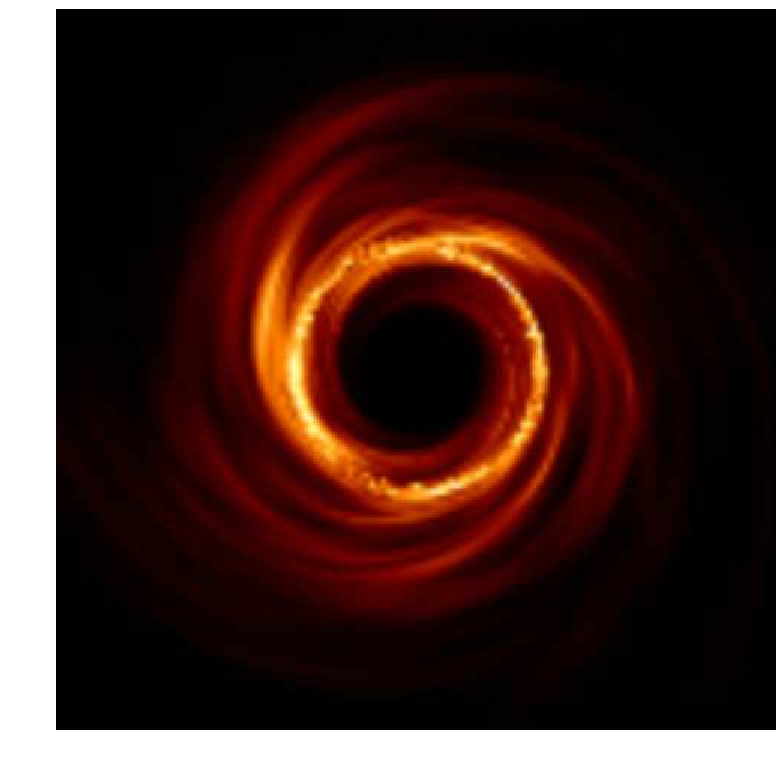
\includegraphics[height=.15\linewidth]{/Users/klbouman/Research/vlbi_imaging/papers/starwarps/9240887pjjjtcdggvxt/figures/compare_var2static/hotakaframe_noaxis.pdf}} } &
			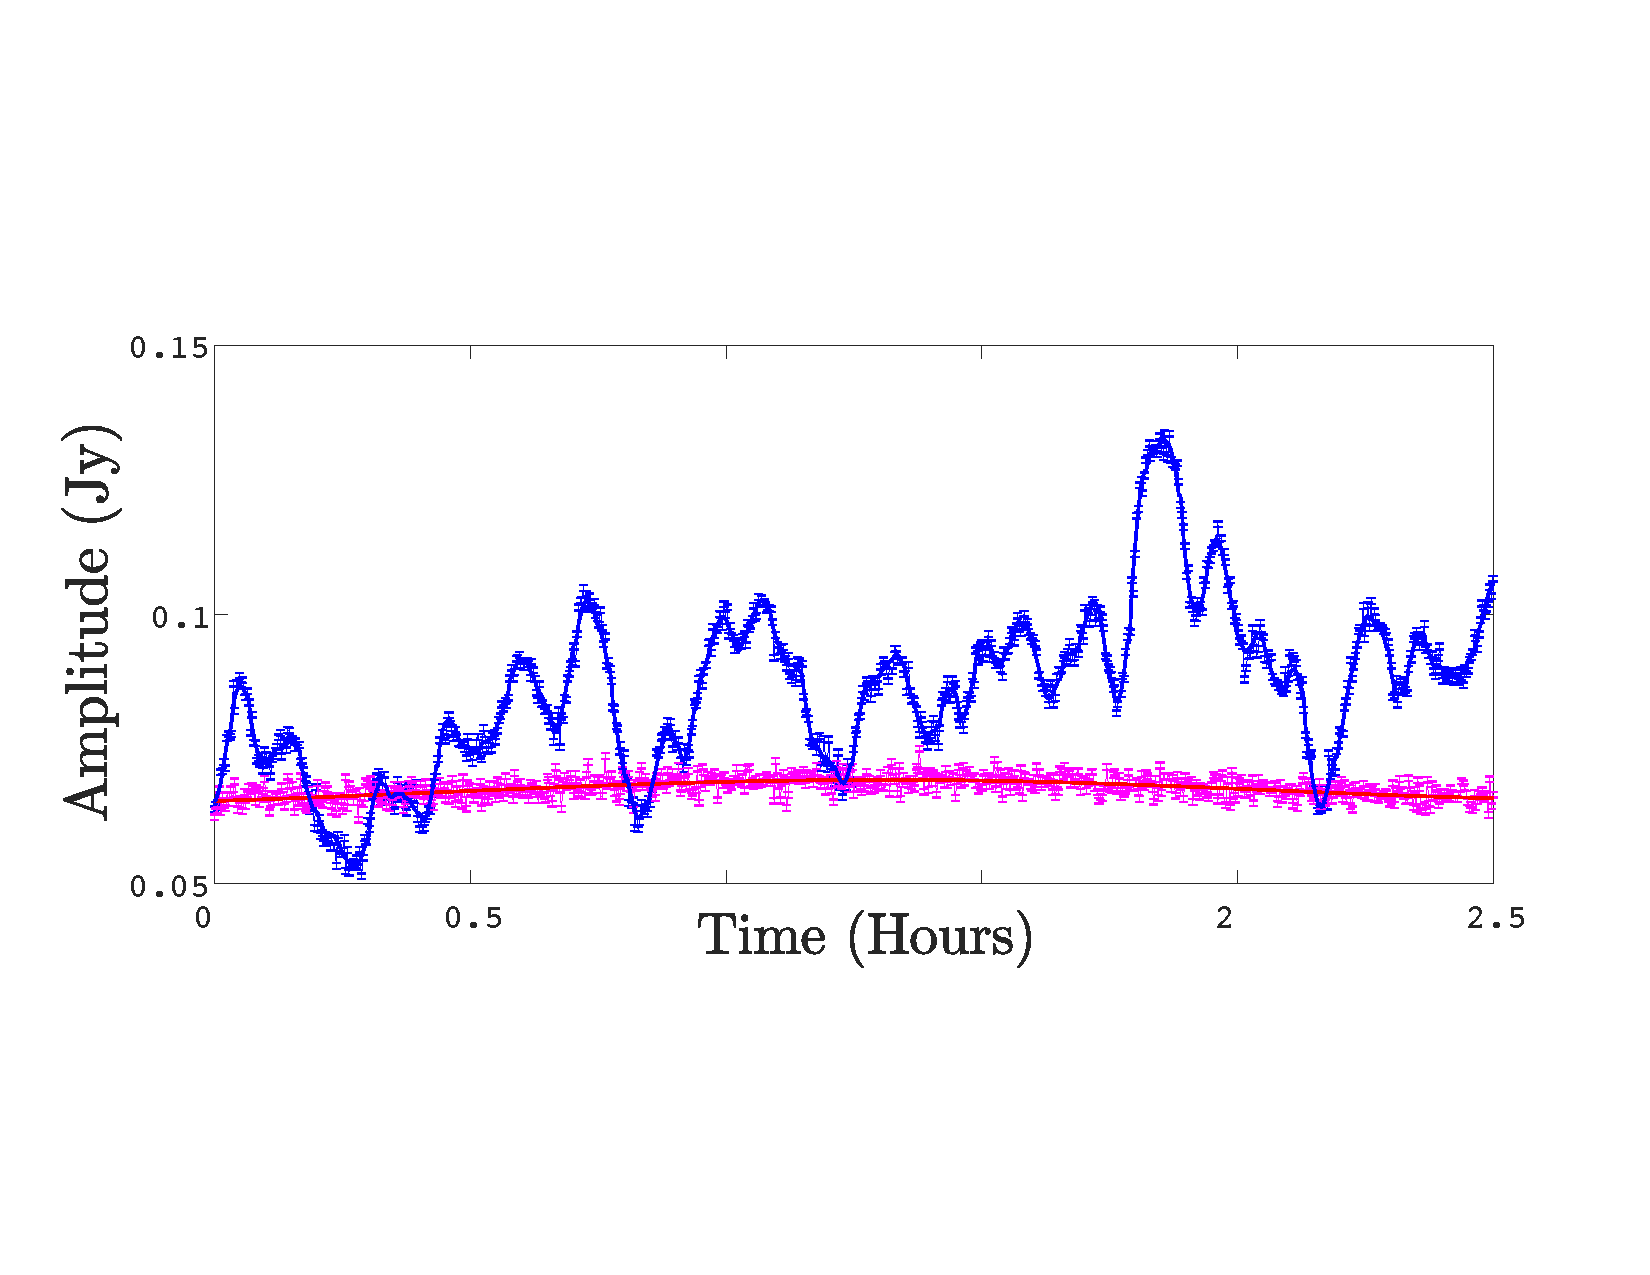
\includegraphics[width=.47\linewidth]{figures/compare_var2static/visamplitudes_notitle_editted.pdf} &
			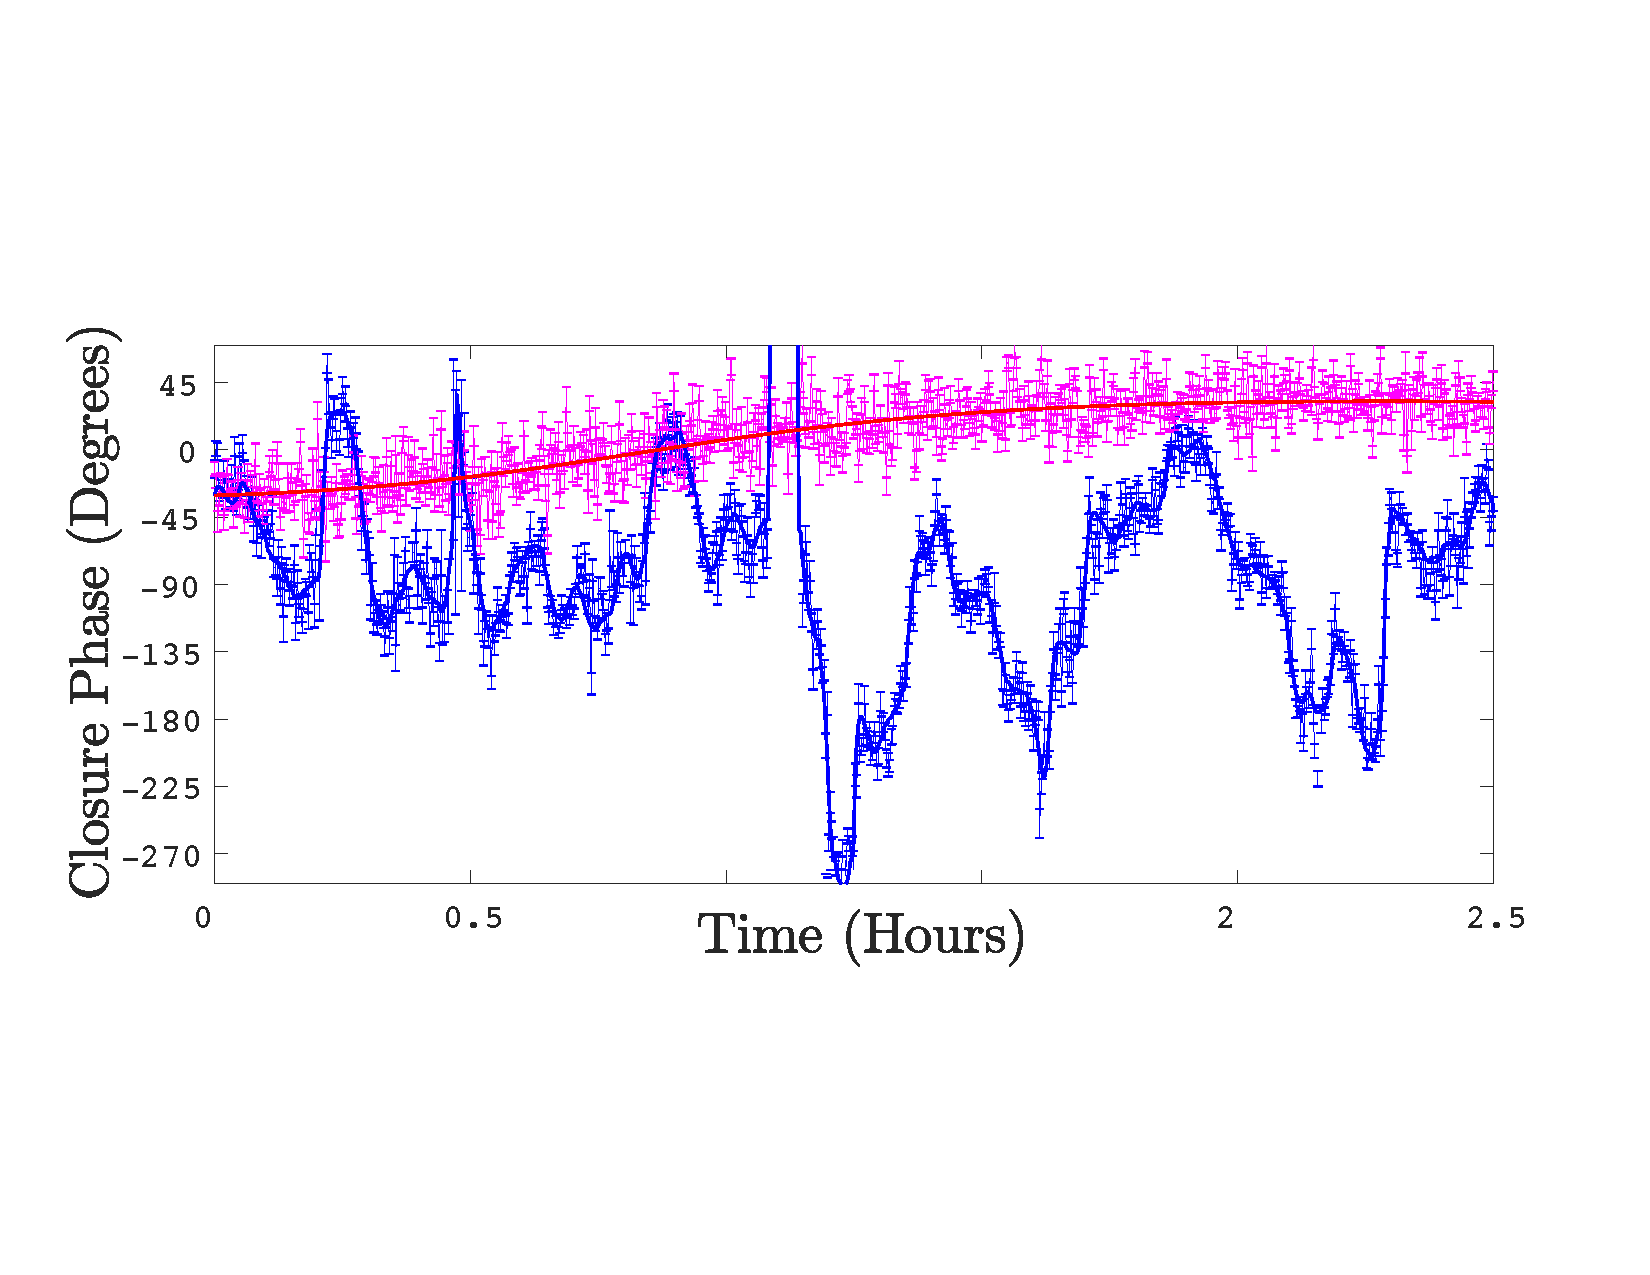
\includegraphics[width=.47\linewidth]{figures/compare_var2static/closurephase_notitle_editted.pdf} 
			\\
		\end{tabular}
		\caption{{\bf Simulated data under a static vs. varying source:} Contrasting of data observed from a static emission region (magenta) to that of a varying emission region (blue) over the course of 2.5 hours. Although both sequences start with the same image, the visibility amplitude and closure phase both begin to deviate from the static image very quickly. The ideal observation for the static and time-varying source is shown by the solid red and blue lines, respectively. We also show sample measurements with their respective error bars in the same colors. This data is simulated at a sampling interval of 11 seconds using the EHT2017 array from the frames in Video 3 presented in Section~\ref{sec:results}. This figure shows 1 of the ${\nmeas \choose 2}$ possible visibility amplitudes and 1 of ${\nmeas \choose 3}$ possible closure phases (phase of the bispectrum). }
		\label{fig:amplandphase}
	\end{center}
	\vspace{-.2in}
\end{figure*}

%KATIE REMOVED THIS PARAGRAPH
A single-dish telescope is diffraction limited, with an angular resolution dictated by the ratio of wavelength to dish diameter~\cite{TMS}. This governing law limits the highest achievable angular resolution of traditional single-dish telescopes. For example, past observations and simulations suggest that the emission surrounding SgrA* subtends approximately $2.5 \times 10^{-10}$ radians, or $50$ $\mu$-arcseconds~\cite{Doeleman_2008}. Imaging this emission region at $1.3$ mm wavelength would require an impossibly large single-dish telescope with a $13,000$ km diameter. However, simultaneously collecting data from an array of telescopes, called an interferometer, allows us to overcome the single-dish diffraction limit, and create a virtual telescope as large as the maximum distance between telescopes in the array. When these telescopes are distributed globally, using separate clocks and recording systems, this technique is referred to as Very Long Baseline Interferometry (VLBI)~\cite{TMS}. 


An interferometer consists of $\ntele$ telescopes simultaneously observing and recording time-stamped data-streams of light traveling from a common source~\cite{TMS}.
%An interferometer consists of $\ntele$ telescopes simultaneously observing a common source. Each telescope records a time-stamped data-stream of the intensity of light traveling from the astronomical emission.
From these measurements a number of different {\it data products} can be computed. 
% This data 
% is a function of the source image's flux (brightness) distribution, and thus is used to constrain image reconstruction. 
%Therefore, for an evolving source, these data products often change erratically over short periods of time (Figure~\ref{fig:amplandphase}).
Depending on the imaging technique and the quality of the measurements, different data products may be used. In this section we review a number of common data products used in VLBI imaging, and throughout this paper. 

%We review the different types of data products, and how we BLAH BLAH BLAH. 

%\begin{align}
%f(x): \Re^{ M^2 \times 1} \rightarrow \Re^{ | y | \times 1 }
%\end{align}

\vspace{-.2in}
\subsection{Visibilities }
\label{sec:vis}


%An interferometer consists of $\ntele$ telescopes simultaneously observing a common source. 
The time-averaged cross-correlation of the recorded scalar electric fields at two telescopes, called a {\it visibility}, provides information about the spatial structure of the observed source\footnote{Although the particular length of time-averaging varies per experiment, for the EHT data is averaged over sub-second intervals before additional coherent averaging is done to increase SNR (on an order of 5-100 seconds).}. Formally, the van Cittert-Zernike theorem states that a visibility, $\vis(I, u,v)$ is related to the ideal source image $I(\xpos, \ypos)$ through a Fourier transform: 
\begin{align}
\vis(I, u,v) \approx \int_{\xpos} \int_{\ypos} e^{-i2 \pi (u\xpos + v \ypos) } I(\xpos, \ypos) d\xpos d\ypos
\label{eq:vcz}
\end{align}
\noindent{where $(\xpos,\ypos)$ is the angular sky coordinate in radians, and $(u,v)$ is the dimensionless baseline vector between two telescopes, measured in wavelengths and orthogonal to the source direction~\cite{TMS}. Note that each visibility is a complex value with both an amplitude and a phase. As each visibility is calculated from a pair of telescopes, for a $\ntele$ telescope array we can obtain up to $\frac{\ntele (\ntele - 1)}{2}$ visibility measurements at a single instant in time. The image spatial frequency sampled by a visibility is related to the distance between the telescopes; telescopes that are father apart inform us about higher spatial frequencies of the underlying image.}
For radio wavelengths, the thermal noise appearing on perfectly calibrated visibilities is 
circularly Gaussian in the real-imaginary plane\footnote{In practice, the thermal noise is calculated from first principles using measured SEFD values at each telescope (see Eq~\ref{eq:thermal}) or estimated empirically. }~\cite{taylor1999synthesis}.


%Note, that the frequency of a visibility is related to the distance between the telescopes; and the resolution of the underlying image sampled by the interferometer is governed by the maximum distance between telescopes in the array. 


%are located the finer the structure they inform on for the source emission. 

%\subsection{Earth Rotation Synthesis}


\vspace{-.1in}
\subsection{Bispectrum and Closure Phases }
\label{sec:bispec}

%For instance, at these short wavelengths, rapidly varying inhomogeneities in the atmosphere introduce additional measurement errors

The van Cittert-Zernike theorem (Equation~\ref{eq:vcz}) is derived under the assumption that light is moving through a vacuum. 
%In all equations and derivations above it was assumed that light was moving through a vacuum. 
However, in reality, inhomogeneity in the Earth's atmosphere causes the light to move at different velocities towards each telescope. At short observing wavelengths, this propagation delay has a large effect on the phase of measurements, and renders the absolute visibility phase unusable for image reconstruction~\cite{monnier2013radio}. Although absolute phase measurements cannot be used, a property called phase closure allows us to still obtain some information from these phases. 

Consider three telescopes, denoted by $i, j$, and $k$, observing the same source. From each pair of telescopes we compute a visibility: $\vis_{i,j}, \vis_{j,k}, \vis_{k,i}$. Rapidly changing atmospheric propagation delays, resulting in phase errors of $\phi_i$ and $\phi_j$ to telescopes $i$ and $j$ respectively, will cause error in the visibility's phase: 
\begin{equation} \vis_{i,j}^{\mbox{\tiny{meas}}} = e^{i(\phi_i - \phi_j)}\vis_{i,j}^{\mbox{\tiny{ideal}}}. 
\end{equation}
\noindent{However, by multiplying the visibilities from 3 different telescopes in a closed loop, we obtain a term that is invariant to the atmosphere (Equation~\ref{eq:phaseclosure})~\cite{jennison}.   }
\begin{align}  
\notag \vis^{\mbox{\tiny{meas}}}_{i,j}\vis^{\mbox{\tiny{meas}}}_{j,k}\vis^{\mbox{\tiny{meas}}}_{k,i} &= e^{i(\phi_i-\phi_j)}\vis^{\mbox{\tiny{ideal}}}_{i,j}e^{i(\phi_j-\phi_k)}\vis^{\mbox{\tiny{ideal}}}_{j,k}e^{i(\phi_k-\phi_i)}\vis^{\mbox{\tiny{ideal}}}_{k,i} \\
%& = e^{i(\phi_i-\phi_j+\phi_j-\phi_k + \phi_k-\phi_i)}\vis^{\mbox{\tiny{true}}}_{i,j}\vis^{\mbox{\tiny{true}}}_{j,k}\vis^{\mbox{\tiny{true}}}_{k,i} \\
&=\vis^{\mbox{\tiny{ideal}}}_{i,j}\vis^{\mbox{\tiny{ideal}}}_{j,k}\vis^{\mbox{\tiny{ideal}}}_{k,i}. %= B_{i,j,k}
\label{eq:phaseclosure}
 \end{align}

We refer to the multiplication of these three complex visibilities in a closed loop 
%$( B_{i,j,k} = \vis^{\mbox{\tiny{true}}}_{i,j}\vis^{\mbox{\tiny{true}}}_{j,k}\vis^{\mbox{\tiny{true}}}_{k,i} ) $ 
as the {\it bispectrum}, and the phase of the bispectrum %$\angle{ \bispec }$ 
as the {\it closure phase}.
Although these data products are invariant to atmospheric noise, they come at the cost of having a fewer number of independent data points - only $\frac{(\ntele-1)(\ntele-2)}{2}$ compared to  $\frac{\ntele(\ntele-1)}{2}$ independent visibilities. Additionally, when using these data products, information related to the absolute location of the source is lost. 

As each bispectrum (Eq.~\ref{eq:phaseclosure}) is the multiplication of three visibilities with Gaussian noise, its noise is not Gaussian. 
Although the noise cannot be fully expressed simply with a covariance matrix, we follow~\cite{bouman2016computational} and approximate the bispectrum's distribution as Gaussian with a best-fit covariance matrix.
%Although the bispectrum noise cannot be expressed simply with a covariance matrix, the noise can be approximated with a best-fit covariance~\cite{bouman2016computational}. 
Refer to the supplemental material for a derivation of this approximation. 

%As each bispectrum is the multiplication of three Gaussian random variables, it is not itself a Gaussian random variable. Although the noise on each bispectrum cannot be expressed simply as a covariance, we can approximate the noise by finding the best fit covariance using the method described in BLAH.

%Recall that each pair of telescopes at a given time is associated with a single $(u,v)$ vector, and that 3 telescopes correspond with $(u,v)$ vectors that form a closed triangle. Therefore, we write this term as:

%\begin{align}
%\bispec(I, u_1, v_1, u_2, v_2) = \vis(I, u_1, v_1) \vis(I, u_2, v_2) \vis (I, u_1 - u_2, v_1 - v_2)
%\end{align}

 
 
\vspace{-.1in}
\subsection{Visibility Amplitudes }
\label{sec:visamp}

%In addition to causing rapid fluctuation of the phase, atmospheric inhomogeneity also introduces fluctuations on the visibility amplitude. 


%Although atmospheric inhomogeneity causes substantial phase errors in the complex visibility, with careful calibration, the visibility's amplitude can be much more accurately estimated. 



%Constraining image reconstruction using the bispectrum's phase closure property is essential in recovering the image's phase. However, in addition to 

Bispectrum measurements not only entangle the phase, but also the amplitudes of the three corresponding spatial frequency components. 
Although atmospheric inhomogeneity causes substantial phase errors in each complex visibility, with careful calibration the amplitude of the visibility can be well estimated. Thus, we have found that during image reconstruction it is quite helpful to additionally constrain the visibility amplitude in addition to the bispectrum or closure phase. Empirically we have found this to be especially important when reconstructing an image with a large field of view. 
%The {\it visibility amplitude} of visibility $\vis(I,u,v)$ is defined by 
%\begin{align}
%| \vis(I,u,v) | = \sqrt{\Re \left[ \vis(I,u,v)\right]^2 + \Im \left[ \vis(I,u,v)\right]^2}
%\end{align}
%\noindent{where $\Re[x]$ and $\Im[x]$ extract the real and imaginary portion of $x$, respectively.}
As thermal noise is isotropic in the real-imaginary plane, a perfectly gain-calibrated visibility amplitude has the same standard deviation of noise as a perfectly calibrated complex visibility \cite{TMS}. 
%Although not used in this work, a convex solution that recovers an image solely from the squared amplitude of the visibilities is discussed in~\cite{demanet}.




%!TEX root = all.tex
% ******************************************************************
% ** Title:            The 2-category theory of quasi-categories
% **                  Background
% ** Precis:        
% ** Author:           Emily Riehl and Dominic Verity
% ** Commenced:        2/3/2012
% ******************************************************************



  \section{Background on quasi-categories}\label{sec:background}

	We start by reviewing some basic concepts and notations. 

  \begin{obs}[size]\label{obs:size-conventions}
    In this paper matters of size will not be of great importance. However, for definiteness we shall adopt the usual conceit of assuming that we have fixed an inaccessible cardinal which then determines a corresponding Grothendieck universe, members of which will be called {\em sets\/}; we refer to everything else as {\em classes}.  A category is {\em small\/} if it has sets of objects and arrows; a category is {\em locally small\/} if each of its hom-sets is small. We shall write $\Set$ to denote the large and locally small category of all sets and functions between them.

    When discussing the existence of limits and colimits we shall implicitly assume that these are indexed by small categories. Correspondingly, completeness and cocompletess properties will implicitly reference the existence of small limits and small colimits.
     \end{obs}

    \subsection{Some standard simplicial notation}\label{subsect:simplicial.notation}

    \begin{ntn}[simplicial operators]\label{ntn:simp.op}
        As usual, we let $\Del+$ denote the algebraists' (skeletal) category of all finite ordinals and order preserving maps between them and let $\Del$ denote the topologists' full subcategory of non-zero ordinals. Following tradition, we write $[n]$ for the ordinal $n+1$ as an object of $\Del+$ and refer to arrows of $\Del+$ as {\em simplicial operators}.  We will generally use lower case Greek letters $\alpha,\beta,\gamma\colon[m]\to[n]$ to denote simplicial operators. We will also use the following standard notation and nomenclature throughout:
        \begin{itemize}
            \item The injective maps in $\Del+$ are called {\em face operators}. For each $j\in[n]$,  $\face_n^j\colon[n-1]\to[n]$ denotes the {\em elementary face operator\/} distinguished by the fact that its image does not contain the integer $j$.
            \item The surjective maps in $\Del+$ are called {\em degeneracy operators}. For each $j\in[n]$, we write $\degen_n^j\colon[n+1]\to[n]$ to denote the {\em elementary degeneracy operator} determined by the property that two integers in its domain map to the integer $j$ in its codomain.
      %  \item We write $\tdegen_n\colon[n]\to[0]$ and $\aug_n\colon[-1]\to[n]$ to denote the unique such simplicial operators.
        \end{itemize}
        Unless doing so would introduce an ambiguity, we tend to reduce notational clutter by dropping the subscripts of these elementary operators.
    \end{ntn}

    \begin{ntn}[(augmented) simplicial sets]\label{ntn:simplicial-sets}
        Let $\sSet$ denote the functor category $\Set^{\Del\op}$,  the category of all {\em simplicial sets\/} and {\em simplicial maps\/} between them. 

        If $X$ is a simplicial set then $X_n$ will denote its value at the object $[n]\in\Del$, called its set of $n$-simplices, and if $f\colon X\to Y$ is a simplicial map then $f_n\colon X_n\to Y_n$ denotes its component at $[n]\in\Del$.

        It is common to think of simplicial sets as being right $\Del$-sets and use the (right) action notation $x\cdot\alpha$ to denote the element of $X_n$ obtained by applying the image under $X$ of a simplicial operator $\alpha \colon [n] \to [m]$ to an element $x\in X_m$. Exploiting this notation,  the functoriality of a simplicial set $X$ may be expressed in terms of the familiar action axioms $(x\cdot\alpha)\cdot\beta = x\cdot(\alpha\circ\beta)$ and $x\cdot\id = x$ and the naturality of a simplicial map $f\colon X\to Y$ corresponds to the action preservation identity $f(x\cdot\alpha)=f(x)\cdot\alpha$. 

A subset $Y\subseteq X$ of a simplicial set $X$ is said to be a {\em simplicial subset\/} of $X$ if it is closed  under  right action by all simplicial operators. If $S$ is a subset of $X$ then there is a smallest simplicial subset of $X$ containing $S$, the simplicial subset of $X$ {\em generated by\/} $S$.

We adopt the same notational conventions for {\em augmented simplicial sets}, objects of the functor category $\Set^{\Del+\op}$, which we denote by $\asSet$.
    \end{ntn}

    \begin{rec}[augmentation]\label{rec:augmentation}
       There is a canonical forgetful functor $\asSet\to\sSet$ constructed by pre-composition with the inclusion functor $\Del\inc\Del+$. Rather than give this functor a name, we prefer instead to allow context to determine whether an augmented simplicial set should be regarded as being a simplicial set by forgetting its augmentation. 

        Left and right Kan extension along $\Del\inc\Del+$ provides left and right adjoints to this forgetful functor, both of which are fully faithful. The left adjoint gives a simplicial set $X$ the {\em initial augmentation\/} $X\to\cpts X$ by its set of path components. The right adjoint gives $X$ the {\em terminal augmentation\/} $X\to {*}$ by the singleton set. We say that an augmented simplicial set is {\em initially\/} (resp.~{\em terminally}) {\em augmented\/} if the counit (resp.~unit) of the appropriate adjunction is  an isomorphism.

        Each $(-1)$-simplex $x$ in an augmented simplicial set $X$ is associated with a terminally augmented sub-simplicial set consisting of those simplices whose $(-1)$-face is $x$. These components are mutually disjoint and their disjoint union is the whole of $X$, providing a canonical decomposition of $X$ as a disjoint union of terminally augmented simplicial sets.
    \end{rec}

    \begin{ntn}[some important (augmented) simplicial sets]

        We fix notation for some important (augmented) simplicial sets. 
        \begin{itemize}
            \item The {\em standard $n$-simplex\/} $\Del^n$ is defined to be the contravariant representable on the ordinal $[n]\in\Del+$. In other words, $\Del^n_m$ is the set of simplicial operators $\alpha\colon[m]\to[n]$ which are acted upon by pre-composition.
            \item The {\em boundary\/} of the standard $n$-simplex $\boundary\Del^n$ is defined to be the simplicial subset of $\Del^n$ consisting of those simplicial operators which are not degeneracy operators. This is the simplicial subset of $\Del^n$ generated by the set of its $(n-1)$-dimensional faces.
            \item The {\em $(n,k)$-horn\/} $\Horn^{n,k}$ (for $n\in\mathbb{N}$ and $0\leq k\leq n$) is the simplicial subset of $\Del^n$ generated by the set $\{\face^i_n\mid 0\leq i\leq n \text{ and } i\neq k\}$ of $(n-1)$-dimensional faces.  Alternatively, we can describe $\Horn^{n,k}$ as the simplicial subset of those simplicial operators $\alpha\colon[m]\to[n]$ for which $\im(\alpha)\cup\{k\}\neq[n]$.
            \item We say that $\Horn^{n,k}$ is an {\em inner horn\/} if $0<k<n$; if $k=0$ or $k=n$, it is an {\em outer horn}.
        \end{itemize}

We have overloaded our notation above to refer interchangeably to objects of $\sSet$ or $\asSet$. There is no ambiguity since in each case the underlying simplicial set of one of these objects in $\asSet$ is  the corresponding object in $\sSet$. As an augmented simplicial set each of the objects above is terminally augmented.

        When $\alpha\colon [n]\to [m]$ is a simplicial operator we use the same symbol to denote the corresponding simplicial map $\alpha\colon\Del^n\to\Del^m$ which acts by post-composing with $\alpha$. In particular, $\face^j_n\colon\Del^{n-1}\to\Del^n$, $\degen^j_n\colon\Del^{n+1}\to\Del^n$,  $\tdegen_n\colon\Del^n\to\Del^0$, and $\aug_n:\Del^{-1}\to\Del^n$ denote the simplicial maps corresponding to the simplicial operators introduced in~\ref{ntn:simp.op} above.
    \end{ntn}

    \begin{ntn}[faces of \protect{$\Del^n$}]\label{ntn:faces-by-vertices}
It is useful to identify a non-degenerate simplex in the standard $n$-simplex $\Delta^n$ simply by naming its vertices. We use the notation $\fbv{v_0,v_1,v_2,...,v_m}$ to denote the simplicial operator $[m]\to [n]$ which maps $i\in[m]$ to $v_i\in[n]$. Let $\Del^{\fbv{v_0,v_1,...,v_m}}$ denote the smallest simplicial subset of $\Del^n$ which contains the face $\fbv{v_0,v_1,...,v_m}$.

      %More generally, in the case where $X$ is a simplicial set whose simplices are {\em determined by their vertices}, in the sense that if $x, x'\in X$ are simplices with the same $0$-faces then $x=x'$, we shall adopt the convention of annotating an $n$-simplex of $X$ by listing its $0$-faces in order $\fbv{x_0,x_1,...,x_n}$. The nerves of pre-ordered sets have simplices which are determined by their vertices and the class of all such simplicial sets is closed under product and subset. Indeed, any simplicial set in this class may be obtained, up to isomorphism, as a simplicial subset of a nerve of a pre-ordered set.
    \end{ntn}
    
    \begin{ntn}[internal hom]\label{ntn:simplicial-hom-space}
    Like any presheaf category, the category of simplicial sets is cartesian closed. We write $Y^X$ for the exponential, equivalently the {\em internal hom\/} or simply {\em hom-space}, from $X$ to $Y$. By the defining adjunction and the Yoneda lemma, an $n$-simplex in $Y^X$ is a simplicial map $X \times \Del^n \to Y$. Its faces and degeneracies are computed by pre-composing with the appropriate maps between the representables.
    \end{ntn}
    
    \subsection{Quasi-categories}

    \begin{defn}[quasi-categories]
      A {\em quasi-category} is a simplicial set $A$ which possesses the {\em right lifting property\/} with respect to all {\em inner horn inclusions\/} $\Horn^{n,k}\inc\Del^n$ ($n \geq 2$, $0<k<n$). A simplicial map between quasi-categories will be called a {\em functor}. We write $\qCat$ for the full subcategory of $\sSet$ consisting of the quasi-categories and functors.
    \end{defn}
    

    \begin{rec}[the homotopy category]\label{rec:hty-category}
      Let $\Cat$ denote the category of all small categories and functors between them. There is an adjunction
      \begin{equation*}
        \adjdisplay \ho-|\nrv:\Cat->\sSet. 
      \end{equation*}
      given by the nerve construction and its left adjoint. Since the nerve construction is fully faithful, we typically regard $\Cat$ as being a full subcategory of $\sSet$ and elide explicit mention of the functor $\nrv$. The nerve of any category is a quasi-category, so we may equally well regard $\Cat$ as being a reflective full subcategory of $\qCat$.

 When $A$ is a quasi-category, $\ho{A}$ is sensibly called its {\em homotopy category}; it has:
 \begin{itemize}
 \item \textbf{objects} the 0-simplices of $A$,
\item \textbf{arrows} equivalence classes of 1-simplices of $A$ which share the same boundaries, and
\item \textbf{composition} determined by the property that $k = g f$ in $\ho{A}$ if and only if there exists a 2-simplex $a$ in $A$ with $a\cdot\face^0=g$, $a\cdot\face^2=f$ and $a\cdot\face^1=k$.
\end{itemize}
See, e.g., \cite[\S 1.2.3]{Lurie:2009fk}. To emphasise the analogy with categories, we draw a 1-simplex $f$ of $A$ as an arrow with domain $f \cdot \face^1$ and codomain $f \cdot \face^0$. With these conventions, a 2-simplex $a$ of $A$ witnessing the identity $k = g f$ in $\ho{A}$ takes the form:
  \begin{equation*}
  \xymatrix{ & \cdot \ar[dr]^g \ar@{}[d]|(.6){a} \\ \cdot \ar[ur]^f \ar[rr]_k & & \cdot}    
\end{equation*} 
      
  Identity arrows in $\ho{A}$ are represented by degenerate 1-simplices. Hence, the composition axiom defines what it means for a parallel pair of 1-simplices  $f,f' \colon x \to y$  to represent the same morphism in $\ho{A}$: this is the case if and only if there exist 2-simplices of each of  (equivalently, any one of) the following forms
  \begin{equation}\label{eq:homotopy-of-1-simplices} \xymatrix{ & y \ar[dr]^{y\cdot \degen^0} & & & y \ar[dr]^{y\cdot\degen^0}& & & x \ar[dr]^f & & & x \ar[dr]^{f'} \\ x \ar[ur]^f \ar[rr]_{f'} & & y & x \ar[ur]^{f'} \ar[rr]_f & & y & x \ar[ur]^{x \cdot\degen^0} \ar[rr]_{f'} & & y & x \ar[ur]^{x\cdot\degen^0} \ar[rr]_f & & y}\end{equation} 
    In this case, we say that $f$ and $f'$ are {\em homotopic relative to their boundary}.
      
Both of the functors $\ho$ and $\nrv$ are {\em cartesian}, preserving all finite products; see \cite[B.0.15]{Joyal:2008tq} or \cite[18.1.1]{Riehl:2014kx}.    
    \end{rec}

\begin{ntn}
 Let $\catone$, $\cattwo$, or $\catthree$  denote the one-point \fbox{$\bullet$}, \emph{generic arrow} \fbox{$\bullet\to\bullet$}, and \emph{generic composed pair} \fbox{$\bullet\to\bullet\to\bullet$} \emph{categories} respectively. Under our identification of categories with their nerves, these categories are identified with the standard simplices $\Del^0$, $\Del^1$, and $\Del^2$ respectively.
\end{ntn}
    

The terms {\em model category\/} and {\em model structure\/}  refer to closed model structures in the sense of Quillen~\cite{Quillen:1967:Model}.

    \begin{rec}[the model category of quasi-categories]\label{rec:qmc-quasicat}
    The quasi-categories are precisely the fibrant-cofibrant objects in a combinatorial model structure on simplicial sets due to Joyal, a proof of which can be found in \cite[\S 6.5]{Verity:2007:wcs1}.
       For our purposes here, it will be enough to recall that Joyal's model structure is completely determined by the fact that it has: 
      \begin{itemize}
      \item {\em weak equivalences\/}, which are  those simplicial maps $w\colon X\to Y$ for which each functor $\ho(A^w)\colon\ho(A^Y)\to\ho(A^X)$ is an equivalence of categories for all quasi-categories $A$,
      \item {\em cofibrations\/}, which are simply the injective simplicial maps. In particular all objects are cofibrant in this model structure, and
      \item {\em fibrations between fibrant objects\/}, which are those functors of quasi-categories which possess the right lifting property with respect to:
      \begin{itemize}
      \item all inner horn inclusions $\Horn^{n,k}\inc\Del^n$ ($n\geq 2$, $0<k<n$), and
      \item (either one of) the monomorphisms $\Del^0\inc \iso$, where $\iso$ denotes the {\em generic isomorphism category\/} $\bullet\cong\bullet$.
      \end{itemize}
      To emphasise the analogy with 1-category theory, we call the fibrations between fibrant objects {\em isofibrations}.
      \end{itemize}
    \end{rec}

The Joyal model structure for quasi-categories is \emph{cartesian}, the meaning of which requires the following construction.


\begin{rec}[Leibniz constructions]\label{rec:leibniz}
If we are given a bifunctor
$ \otimes \colon \lcat{K} \times \lcat{L} \to \lcat{M}$ 
  whose codomain  possesses all pushouts, then the {\em Leibniz construction\/} provides us with a bifunctor $ \leib\otimes \colon \lcat{K}\mapcat \times \lcat{L}\mapcat \to \lcat{M}\mapcat$
  between arrow categories, which carries a pair of objects $f \in \lcat{K}\mapcat$ and $g \in \lcat{L}\mapcat$ to an object $f\leib\otimes g \in \lcat{M}\mapcat$ defined to be the map induced by the universal property of the pushout in the following diagram:
  \begin{equation}
  \xymatrix@=2em{
    {K\otimes L} \ar[d]_{K\otimes g} \ar[r]^{f\otimes L} &
    {K'\otimes L} \ar[d] \ar@/^4ex/[ddr]^{K'\otimes g} & \\
    {K\otimes L'} \ar[r] \ar@/_4ex/[rrd]_{f\otimes L'} &
    {(K'\otimes L) \cup_{K\otimes L} (K\otimes L') } \poexcursion
    \ar@{-->}[dr]_{f\leib\otimes g} & \\
    & & {K'\otimes L'}
  }
  \end{equation}
  The action of this functor on the arrows of $\lcat{K}\mapcat$ and $\lcat{L}\mapcat$ is the canonical one induced by the functoriality of $\otimes$ and the universal property of the pushout in the diagram above. In the case where the bifunctor $\otimes$ defines a monoidal product, the Leibniz bifunctor $\leib\otimes$ is frequently called the {\em pushout product}.
In the context of a bifunctor $\hom \colon \lcat{K}\op \times \lcat{L} \to \lcat{M}$, the dual construction, defined using pullbacks in $\lcat{M}$, is preferred.  We refer the reader to \cite[\S\ref*{reedy:sec:Leibniz-Reedy}]{RiehlVerity:2013kx} for a full account of this construction and its properties. %In particular, in the few instances where Reedy category theory is invoked in proofs appearing below, we make use of the notational conventions established therein.  
\end{rec}

\begin{rec}[cartesian model categories]\label{rec:cart-modcat}
The cartesianness of the Joyal model structure may be formulated in the following equivalent forms:
  \begin{enumerate}
    \item If $i\colon X\tcof Y$ and $j\colon U\tcof V$ are both cofibrations (monomorphisms) then so is their {\em Leibniz product\/} $i\leib\times j\colon (Y\times U)\cup_{X\times U} (X\times V)\tcof (Y\times V)$. Furthermore, if $i$  or $j$ is a trivial cofibration then so is $i\leib\times j$.
    \item If $i\colon X\tcof Y$ is a cofibration (monomorphism) and $p\colon A\tfib B$ is a fibration then their {\em Leibniz hom\/} $\leib\hom(i,p)\colon A^Y\tfib B^Y\times_{B^X} A^X$ is also a fibration. Furthermore, if $i$ is a trivial cofibration or $p$ is a trivial fibration then $\leib\hom(i,p)$ is also a trivial fibration.
  \end{enumerate}
  In particular, if $A$ is a quasi-category then we may apply the second of these formulations to the unique isofibration $!\colon A\to 1$ and monomorphisms $\emptyset\inc X$ and $i\colon X\inc Y$ to show that $A^X$ is again a quasi-category and that the pre-composition functor $A^i\colon A^Y\tfib A^X$ is an isofibration. 
\end{rec}

\begin{obs}[closure properties of isofibrations]\label{obs:isofibration-closure}
As a consequence of \ref{rec:qmc-quasicat} and \ref{rec:cart-modcat}, the isofibrations enjoy the following closure properties:
\begin{itemize}
\item  The isofibrations are closed under products, pullbacks, retracts, and transfinite limits of towers (as fibrations between fibrant objects).
\item The isofibrations are also closed under the Leibniz hom $\leib\hom(i,-)$ for any monomorphism $i$ and, in particular, under exponentiation $(-)^X$ for any simplicial set $X$ (as fibrations between fibrant objects in a cartesian model category).
\end{itemize}
\end{obs}

\subsection{Isomorphisms and marked simplicial sets}

  \begin{defn}[isomorphisms in quasi-categories]\label{defn:equivalences} 
    When $A$ is a quasi-category, we say that a 1-simplex $a\in A_1$ is an {\em isomorphism\/} if and only if the corresponding arrow of its homotopy category $\ho{A}$ is an isomorphism in the usual sense.
\end{defn}

Others use the term ``equivalences'' for the isomorphisms in a quasi-category, but we believe our terminology is less ambiguous: no stricter notion of isomorphism exists. 

When working with isomorphisms in quasi-categories, it will sometimes be convenient to work in the category of {\em marked simplicial sets\/} as defined by Lurie~\cite{Lurie:2009fk}.

    \begin{defn}[marked simplicial sets]
      A {\em marked simplicial set} $X$ is a simplicial set equipped with a specified subset of \emph{marked} $1$-simplices $mX\subseteq X_1$ containing all the degenerate 1-simplices. A map of marked simplicial sets is a map of underlying simplicial sets that carries marked 1-simplices to marked 1-simplices. While the category $\msSet$ of marked simplicial sets is not quite as well behaved as $\sSet$ it is nevertheless a \emph{quasitopos}, which implies that it is complete, cocomplete, and (locally) cartesian closed (see \cite[Observation 11]{Verity:2007:wcs1} and \cite{Street:2003:WomCats}).

      The functor $\msSet\to\sSet$ which forgets markings has both a left and a right adjoint. This left adjoint, dubbed {\em flat\/} by Lurie, makes a simplicial set $X$ into a marked simplicial set $X^\flat$ by giving it the minimal marking in which only the degenerate $1$-simplices are marked. Conversely, this right adjoint, which Lurie calls {\em sharp}, makes $X$ into a marked simplicial set $X^\sharp$ by giving it the maximal marking in which all $1$-simplices are marked. If $X$ is already a marked simplicial set then we will use the notation $X^\flat$ and $X^\sharp$ for the marked simplicial sets obtained by applying the flat or sharp construction (respectively) to the underlying simplicial set of $X$.

      In general, we will identify simplicial sets with their minimally marked variants, allowing us to extend the notation introduced above to the marked context. Any variation to this rule will be commented upon as we go along.
    \end{defn}
    
        \begin{rmk}[stratified simplicial sets]
Earlier authors, including Roberts~\cite{Roberts:1978:Complicial}, Street~\cite{Street:1987:Oriental}, and Verity~\cite{Verity:2008sr,Verity:2007:wcs1}, have studied a more general notion of {\em stratification}. A {\em stratified simplicial set\/} is again a simplicial set $X$ equipped with a specified subset of simplices which, in that context, are said to be {\em thin}. A stratification may contain simplices of arbitrary dimension and it must again contain all degenerate simplices. Stratifications are used to build structures called {\em complicial sets\/}, which model homotopy coherent higher categories in much the way that quasi-categories model homotopy coherent categories.
    \end{rmk}

    \begin{rec}[products and exponentiation]\label{rec:marked-prod-exp}
The product in $\msSet$ of marked simplicial sets $X$ and $Y$ is formed by taking the product of underlying simplicial sets and marking those $1$-simplices $(x,y)\in X\times Y$ which have $x$ marked in $X$ and $y$ marked in $Y$.

      An exponential (internal hom) $Y^X$ in marked simplicial sets has $n$-simplices which correspond to maps $k\colon X\times\Del^n\to Y$ of marked simplicial sets and has marked $1$-simplices those $k$ which extend along the canonical inclusion $X\times\Del^1\inc X\times(\Del^1)^\sharp$ to give a (uniquely determined) map $k'$ \[\xymatrix{ X \times \Del^1 \ar[r]^-k \ar@{_(->}[d] & Y \\ X \times (\Del^1)^\sharp \ar[ur]_-{k'}}\] That is, a marked 1-simplex in $Y^X$ is a map $k'\colon X \times (\Del^1)^\sharp \to Y$ of marked simplicial sets; see \cite[\S 3.1.3]{Lurie:2009fk}.
     The only $1$-simplices which are not marked in $X\times\Del^1$ but are marked in $X\times(\Del^1)^\sharp$ are pairs of the form $(x,\id_{[1]})$ in which $x$ is marked in $X$. It follows that a marked simplicial map $k\colon X\times\Del^1\to Y$ extends along $X\times\Del^1\inc X\times(\Del^1)^\sharp$, and thus represents a marked $1$-simplex in $Y^X$, if and only if for all marked $1$-simplices $x$ in $X$ the $1$-simplex $k(x,\id_{[1]})$ is marked in $Y$.
    \end{rec}

    \begin{rec}[isomorphisms and markings]\label{rmk:equiv-markings}
A quasi-category $A$ becomes a marked simplicial set $A^\natural$ with the {\em natural marking}, under which a 1-simplex is marked if and only if it is an isomorphism. When we regard an object as being a quasi-category in the marked setting we will always assume that it carries the natural marking without comment. A functor $f\colon A\to B$ between quasi-categories automatically preserves natural markings simply because the corresponding functor $\ho(f)\colon\ho{A}\to\ho{B}$ preserves isomorphisms.
\end{rec}

\begin{ntn}
      In this context it is useful to adopt the special marking convention for horns ($n \geq 1$, $0\leq k \leq n$) under which we
      \begin{itemize}
      \item write $\Del^{n:k}$ for the marked simplicial set obtained from the standard minimally marked simplex $\Del^n$ by also marking the edge $\fbv{0,1}$ in the case $k=0$ and marking the edge $\fbv{n-1,n}$ in the case $k=n$,
      \item inherit the marking of the horn $\Horn^{n,k}$ from that of $\Del^{n:k}$, and
      \item use $\Horn^{n,k}\inc\Del^{n:k}$ to denote the marked inclusion of this horn into its corresponding specially marked simplex.
      \end{itemize}
\end{ntn}

      Using these conventions we may recast Joyal's ``special horn filler'' result \cite[1.3]{Joyal:2002:QuasiCategories} simply as follows.

\begin{prop}[Joyal]\label{prop:joyal-special-horn} A naturally marked quasi-category has the right lifting property with respect to all marked horn inclusions $\Horn^{n,k}\inc\Del^{n:k}$, for $n\geq 1$ and $0\leq k \leq n$.
\end{prop}

 An important corollary is that a Kan complex is precisely a quasi-category in which every 1-simplex is an isomorphism \cite[1.4]{Joyal:2002:QuasiCategories}.

    \begin{rec}[the model structure of naturally marked quasi-categories]\label{rec:qmc-quasi-marked}
There is a model structure on the category of marked simplicial sets whose fibrant-cofibrant objects are precisely the naturally marked quasi-categories (see Lurie~\cite[\S 3.1]{Lurie:2009fk} or Verity~\cite[\S 6.5]{Verity:2007:wcs1}). This model category is  combinatorial and cartesian and is completely characterised by the fact that it has:
      \begin{itemize}
        \item {\em weak equivalences\/} which are those maps $w\colon X\to Y$ of marked simplicial sets for which $\ho(A^w)\colon\ho(A^Y)\to\ho(A^X)$ is an equivalence of categories for all (naturally marked) quasi-categories $A$,
        \item {\em cofibrations\/} which are simply the injective maps of marked simplicial sets, and
        \item {\em fibrations between fibrant objects\/} which are the isofibrations of naturally marked quasi-categories.
      \end{itemize}
      Here, the exponential $A^X$ is the internal hom in the category of marked simplicial sets $\msSet$. The functor $\ho\colon\msSet\to\Cat$ is the left adjoint to the nerve functor $\nrv\colon\Cat\to\msSet$ which carries a category $\scat{C}$ to the marked simplicial set whose underlying simplicial set is the usual nerve and in which a $1$-simplex is marked if and only if it is an isomorphism in $\scat{C} \cong \ho{\scat{C}}$. The left adjoint $h$ sends a marked simplicial set $X$ to the localisation of its homotopy category $hX$ at the set of marked edges. Note that in the case of a naturally marked quasi-category $A^\natural$, $h(A^\natural) = hA$, the usual homotopy category of the quasi-category.

      By \cite[7.14]{Joyal:2007kk}, a cofibration is a weak equivalence if and only if it has the left lifting property with respect to the fibrations between fibrant objects.
        In particular, in this model structure all of the special marked horn inclusions $\Horn^{n,k}\inc\Del^{n:k}$ ($n \geq 1$, $0\leq k\leq n$) and the inclusion $(\Del^1)^\sharp\inc\iso$ of the marked 1-simplex into the naturally marked isomorphism category are trivial cofibrations (see \cite[B.10, B.15]{DuggerSpivak:2011ms}). This proves that an isomorphism $\Del^1 \to A$ in a quasi-category may always be extended to a functor $\iso \to A$ \cite[1.6]{Joyal:2002:QuasiCategories}.
\end{rec}

  \begin{obs}[natural markings, internal homs, and products]\label{obs:nat-mark-homs}
The product of two naturally marked quasi-categories is again a naturally marked quasi-category.
By cartesianness of the marked model structure, if $A$ is a naturally marked quasi-category and $X$ is any marked simplicial set then the exponential $A^X$ is again a naturally marked quasi-category.    In summary, the fully faithful natural marking functor $\natural\colon\qCat\to\msSet$ is a cartesian closed functor, in the sense that it preserves products and internal homs.
    \end{obs}

  The content of observation \ref{obs:nat-mark-homs} is  more profound than one might initially suspect. It might be summarised by the slogan ``a natural transformation of functors is an isomorphism if and only if it is a {\em pointwise isomorphism}''. The precise meaning of this slogan is encoded in the following result.

            \begin{lem}[pointwise isomorphisms are isomorphisms]\label{lem:pointwise-equiv}
Let $X$ be a marked simplicial set and let $A$ be a naturally marked quasi-category.  A $1$-simplex $k\colon X\times\Del^1\to A$ is marked in $A^X$ if and only if for all $0$-simplices $x$ in $X$ the $1$-simplex $k(x\cdot\degen^0,\id_{[1]})$ is marked in $A$.
       \end{lem}
Here is the intuition for this result. The component of a map $k \colon X \times \Del^1 \to A$ at a 1-simplex $f \colon a \to b$ in $X$      is a diagram $\Del^1 \times \Del^1 \to A$ \begin{equation}\label{eq:pointwise-equivalence-square}\xymatrix@=35pt{ \cdot \ar[d]_{k(f,\face^1)} \ar[r]^{k(a,\id_{[1]})} \ar[dr]|{k(f,\id_{[1]})} & \cdot \ar[d]^{k(f,\face^0)} \\ \cdot \ar[r]_{k(b,\id_{[1]})} & \cdot}\end{equation} If $f$ is marked and $k$ is a marked map, then the verticals are marked in $A$. If $A$ is a naturally marked quasi-category, then if the horizontals, the ``components'' of $k$, are marked, then so is the diagonal edge, simply because isomorphisms compose. If this is the case for all marked 1-simplices $f$, then $k$ is marked in $A^X$ by the definition of the internal hom in $\msSet$.
               
      \begin{proof}
As recalled in~\ref{rec:marked-prod-exp}, $k$ is a marked $1$-simplex in $A^X$ if and only if $k(f,\id_{[1]})$ is marked in $A$ for all marked edges $f$ of $X$. In particular, the edges $k(x\cdot\degen^0,\id_{[1]})$ are necessarily marked in $A$ if $k$ is marked in $A^X$. We show that this condition is sufficient to detect the marked edges $k \in (A^X)_1$.

 The $2$-simplex $(f\cdot\degen^0,\degen^1)$ of $X\times\Del^1$ can be drawn as follows:
        \[\left(    \vcenter{
        \xymatrix{ & \cdot \ar[dr]^{f} \ar@{}[d]|(.6){f \cdot \degen^0} \\ \cdot \ar@{=}[ur]^{(f \cdot \face^1)\cdot \degen^0} \ar[rr]_{f} & & \cdot} }\quad,\quad   \vcenter{
        \xymatrix{ & \cdot \ar@{=}[dr]^{\degen^0} \ar@{}[d]|(.6){\degen^1} \\ \cdot \ar[ur]^{{\id_{[1]}}} \ar[rr]_{\id_{[1]}} & & \cdot} } \right) \]
Applying $k$, the $2$-simplex $k(f\cdot\degen^0,\degen^1)$ of $A$ witnesses the fact that $k(f,\id_{[1]})$ is a composite of $k(f,\degen^0)$ and $k((f\cdot\face^1)\cdot\degen^0,\id_{[1]})$. 
        
        Now when $f$ is marked in $X$, the edge $(f,\degen^0)$ is marked in $X\times \Del^1$, so it follows that $k(f,\degen^0)$ is marked in $A$. By assumption the $1$-simplex $k((f\cdot\face^1)\cdot\degen^0,\id_{[1]})$ is also marked in $A$. The isomorphisms, that is to say naturally marked $1$-simplices, compose in $A$ simply because isomorphisms compose in the category $\ho{A}$, so it follows that $k(f,\id_{[1]})$ is marked in $A$. 
    \end{proof}

Recall that the marked edges in a naturally marked quasi-category are precisely the isomorphisms. Reinterpetting Lemma \ref{lem:pointwise-equiv} in the unmarked context, we have proven:

\begin{cor}\label{cor:pointwise-equiv}
For any quasi-category $A$ and simplicial set $X$, an edge $k \in (A^X)_1$ is an isomorphism if and only if each of its components $k(x) \in A_1$, defined by evaluating at each vertex $x \in X_0$, are isomorphisms.
\end{cor}



  \begin{obs}\label{obs:marked-arrow-subcat}
    If $A$ is a naturally marked quasi-category then pre-composition by the inclusion $\Del^1\inc(\Del^1)^\sharp$ gives rise to an inclusion $A^{(\Del^1)^\sharp}\inc A^{\Del^1}$ of naturally marked quasi-categories. Taking transposes, we see that Lemma \ref{lem:pointwise-equiv} may be recast as saying that a marked simplicial map $k\colon X\to A^{\Del^1}$ has a (necessarily unique) lift as the dotted arrow in
    \begin{equation*}
      \xymatrix@=2em{
        & {A^{(\Del^1)^\sharp}}\ar@{u(->}[d] \\
        {X}\ar[r]_{k}\ar@{-->}[ur] &
        {A^{\Del^1}}
      }
    \end{equation*}
    if and only if $k$ maps each 0-simplex $x\in X$ to an object $k(x)\in A^{\Del^1}$ which corresponds to a marked arrow of $A$. In other words, the map $A^{(\Del^1)^\sharp}\inc A^{\Del^1}$ is a fully faithful inclusion which identifies $A^{(\Del^1)^\sharp}$ with the full sub-quasi-category of $A^{\Del^1}$ whose objects are the isomorphisms in $A$.
  \end{obs}

\subsection{Join and slice}\label{subsec:join}

Particularly to facilitate comparisons between our development of the theory of quasi-categories, using the enriched category theories of 2-categories and simplicial categories, and the more traditional accounts following Joyal and Lurie, we review Joyal's slice and join constructions, introduced in \cite{Joyal:2002:QuasiCategories}. Unlike in the classical treatments, these technical combinatorial details will be of secondary importance for us, and for that reason, we encourage the reader to skip this section upon first reading, referring back only as necessary. A more leisurely account of the combinatorial work reviewed here can be found in an earlier version of this paper \cite[\S A]{RiehlVerity:2015tt-v3}.

  \begin{defn}[joins and d{\'e}calage]\label{defn:join-dec} The algebraists' skeletal category $\Del+$ of all finite ordinals and order preserving maps supports a canonical strict (non-symmetric) monoidal structure $(\Del+,\oplus,[-1])$ in which $\oplus$ denotes the {\em ordinal sum\/} given 
  \begin{itemize}
    \item for objects $[n],[m]\in\Del+$ by $[n]\oplus[m] \defeq [n+m+1]$,
    \item for arrows $\alpha\colon[n]\to[n'], \beta\colon[m]\to[m']$ by $\alpha\oplus\beta\colon[n+m+1]\to[n'+m'+1]$ defined by
  \begin{equation*}
    \alpha\oplus\beta(i) =
    \begin{cases}
    \alpha(i)& \text{if $i\leq n$,} \\
    \beta(i-n-1) + n' + 1& \text{otherwise.}
    \end{cases}
  \end{equation*}
  \end{itemize}
By Day convolution, this bifunctor extends to a (non-symmetric) monoidal closed structure $(\asSet, \join, \Del^{-1}, \dec_l, \dec_r)$ on the category of augmented simplicial sets. Here the monoidal operation $\join$ is known as the {\em simplicial join\/} and its closures $\dec_l$ and $\dec_r$ are known as the {\em left and right d{\'e}calage constructions}, respectively.   To fix handedness, we declare that for each augmented simplicial set $X$ the functor $\dec_l(X,{-})$ (resp.\ $\dec_r(X,{-})$) is right adjoint to $X\join{-}$ (resp.\ ${-}\join X$).

The join $X\join Y$ of augmented simplicial sets $X$ and $Y$ may be described explicitly as follows:
  \begin{itemize}
    \item it has simplices pairs $(x,y) \in (X\join Y)_{r+s+1}$ with $x\in X_r$, $y\in Y_s$,
    \item if $(x,y)$ is a simplex of $X\join Y$ with $x \in X_r$ and $y \in Y_s$ and $\alpha\colon[n]\to[r+s+1]$ is a simplicial operator in $\Del+$, then $\alpha$ may be uniquely decomposed as $\alpha=\alpha_1\join\alpha_2$ with $\alpha_1\colon[n_1]\to[r]$ and $\alpha_2\colon[n_2]\to[s]$, and we define $(x,y)\cdot\alpha\defeq (x\cdot\alpha_1,y\cdot\alpha_2)$. 
  \end{itemize}
If $f\colon X\to X'$ and $g\colon Y\to Y'$ are simplicial maps then the simplicial map $f\join g\colon X\join Y\to X'\join Y'$  carries the simplex $(x,y)\in X\join Y$ to the simplex $(f(x),g(y))\in X'\join Y'$. 
  \end{defn}

  \begin{defn}[d{\'e}calage and slices]\label{defn:slices}
The d{\'e}calage functors can be used to define Joyal's \emph{slice} construction for a map $f\colon X\to A$ of simplicial. 
Fixing a simplicial set $X$ and identifying the category $\sSet$  of simplicial sets with the full subcategory of terminally augmented simplicial sets in $\asSet$, we define a functor
    \begin{equation*}
      {-}\mathbin{\bar\join} X\colon \xy<0em,0em>*+{\sSet}\ar <6em,0em>*+{X\slice\sSet}\endxy\mkern30mu
      (\text{resp.\ } 
      X\mathbin{\bar\join}{-}\colon \xy<0em,0em>*+{\sSet}\ar <6em,0em>*+{X\slice\sSet}\endxy)
    \end{equation*}
    which carries a simplicial set $Y\in\sSet$ to the object ${*}\join X\colon X\cong\Del^{-1}\join X\to Y\join X$ (resp.\ $X\join{*}\colon X\cong X\join\Del^{-1} \to X\join Y$) induced by the map ${*}\colon\Del^{-1}\to Y$ corresponding to the unique $(-1)$-simplex of $Y$. This functor preserves all colimits, and thus admits a right adjoint that we now describe explicitly.
    
Observe that the $(-1)$-dimensional simplices of $\dec_r(X, A)$ (resp.\ $\dec_l(X,A)$) are in bijective correspondence with simplicial maps $f\colon X\to A$. So if we are given such a simplicial map we may, by recollection \ref{rec:augmentation}, extract the component of $\dec_r(X,A)$ (resp.\ $\dec_l(X,A)$) consisting of those simplices whose $(-1)$-face is $f$, which we denote by $\slicer{A}{f}$ (resp.\ $\slicel{f}{A}$) and call the {\em slice of $A$ over (resp.\ under) $f$}. Now it is a matter of an easy calculation to demonstrate directly that $\slicer{A}{f}$ (resp. $\slicel{f}{A}$) has the universal property required of the right adjoint to ${-}\bar\join X$ (resp.\ $X\bar\join {-}$) at the object $f\colon X\to A$ of $X\slice\sSet$.

    In other words, these d{\'e}calages admit the following canonical decompositions as disjoint unions of (terminally augmented) slices: 
    \begin{equation*}
      \dec_r(X,A)=\bigsqcup_{f\colon X\to A} (\slicer{A}{f})\mkern30mu
      \dec_l(X,A)=\bigsqcup_{f\colon X\to A} (\slicel{f}{A})
    \end{equation*}

    We think of the slice $\slicel{f}{A}$ as being the simplicial set of {\em cones under the diagram $f$\/} and we think of the dual slice $\slicer{A}{f}$ as being the simplicial set of {\em cones over the diagram $f$}.
  \end{defn}
  
  \begin{obs}[slices of quasi-categories]\label{obs:slice-and-qcats}
    A direct computation from the explicit description of the join construction given above demonstrates that the Leibniz join (see recollection~\ref{rec:leibniz}) of a horn and a boundary $(\Horn^{n,k}\inc\Del^n)\leib\join(\boundary\Del^m\inc\Del^m)$ is again isomorphic to a single horn $\Horn^{n+m+1,k}\inc\Del^{n+m+1}$. Dually the Leibniz join $(\boundary\Del^n\inc\Del^n)\leib\join(\Horn^{m,k}\inc\Del^m)$ is isomorphic to the single horn $\Horn^{n+m+1,n+k+1}\inc\Del^{n+m+1}$. 

    Combining these computations with the properties of the Leibniz construction developed in \cite[\S\ref*{reedy:sec:Leibniz-Reedy}]{RiehlVerity:2013kx}, we may show that an augmented simplicial set $A$ has the right lifting property with respect to all (inner) horn inclusions then so do the left and right d{\'e}calages $\dec_l(X,A)$ and $\dec_r(X,A)$ for any augmented simplicial set $X$. In particular, this tells us that if $f\colon X\to A$ is any map of simplicial sets and $A$ is a quasi-category then the slices $\slicel{f}{A}$ and $\slicer{A}{f}$ are also quasi-categories. 

    Working in the marked context, we may extend this result to Leibniz joins with specially marked outer horns. That then allows us to prove that if $p\colon A\to B$ is an isofibration of quasi-categories and $f\colon X\to A$ is any simplicial map then the induced simplicial maps $p\colon \slicer{A}{f}\to \slicer{B}{pf}$ and $p\colon \slicel{f}{A}\to \slicel{pf}{B}$ are also isofibrations of quasi-categories.
  \end{obs}

A variant of the join and slice constructions, also due to Joyal, is more closely related to the enriched categorical comma constructions that we will use here.

 \begin{defn}[fat join]\label{def:fat-join}
    We define the {\em fat join} of two simplicial sets $X$ and $Y$ to be the simplicial set $X\fatjoin Y$ constructed by means of the following pushout:
    \begin{equation}\label{eq:fat-join-def}
      \xymatrix@R=2em@C=4em{
        {({X}\times{Y})\sqcup({X}\times{Y})}\ar[r]^-{\pi_X\sqcup\pi_Y}
        \ar[d]_{\langle{X}\times\face^1\times{Y},
          {X}\times\face^0\times{Y}\rangle} &
        {{X}\sqcup{Y}}\ar[d] \\
        {{X}\times\Del^1\times{Y}} \ar[r] &
        {{X}\fatjoin{Y}}\poexcursion
      }
    \end{equation}
    We may extend this construction to simplicial maps in the obvious way to give us a bifunctor $\fatjoin\colon\sSet\times\sSet\to\sSet$, and it is clear that this preserves connected colimits in each variable. It does not preserve all colimits  because the coproduct bifunctor $\sqcup$ (as used in the top right hand corner of the defining pushout above) fails to preserve coproducts  in each variable (while it does preserve connected colimits). In particular, a fat join of a simplicial set $X$ with the empty simplicial set, rather than being empty, is isomorphic  to $X$ itself.

%    Now if we again identify the category of simplicial sets $\sSet$ with the full subcategory of terminally augmented simplicial sets then we may extend our fat join to a bifunctor on augmented simplicial sets. To do this we start by observing that every augmented simplicial set $X$ may be written canonically as a coproduct $\bigsqcup_{i\in I} X_i$ in $\asSet$ of terminally augmented simplicial sets. So if $X = \bigsqcup_{i\in I} X_i$ and $Y=\bigsqcup_{j\in J} Y_j$ are two augmented simplicial sets with terminally augmented components $X_i$ and $Y_j$, then we define $X\join Y$ to be the coproduct $\bigsqcup_{i\in I, j\in J} X_i\fatjoin Y_j$ in $\asSet$. We extend this to maps of augmented simplicial sets in the obvious way, using the fact that we may decompose such maps into families of maps between terminally augmented components. It is now a routine matter to verify that, when regarded as being a bifunctor on $\asSet$, the fat join does indeed preserve {\em all\/} colimits in each variable. Consequently, since $\asSet$ is a presheaf category, it follows that the fat join bifunctor on $\asSet$ has both left and right closures $\fatdec_l(X,A)$ and $\fatdec_r(X,A)$, called  {\em left and right fat d{\'e}calage\/} respectively, which notation we fix by declaring that if $X$ is an augmented simplicial set then $X\fatjoin{-}\dashv\fatdec_l(X,{-})$ and ${-}\fatjoin X\dashv\fatdec_r(X,{-})$.

The fat join of two non-empty simplicial sets $X$ and $Y$ may be described more concretely as the simplicial set obtained by taking the quotient of ${X}\times\Del^1\times{Y}$ under the simplicial congruence relating the pairs of $r$-simplices
    \begin{equation}\label{eq:fat-join-cong}
    (x,0,y)\sim (x,0,y')\quad \text{and}\quad (x,1,y) \sim (x',1,y) 
   \end{equation}
   where $0$ and $1$ denote the constant operators $[r]\to[1]$. We use square bracketed triples $[x,\beta,y]_\sim$ to denote equivalence classes under $\sim$. 
  \end{defn}

  \begin{defn}[fat slice]\label{defn:fat-slices}
    Replaying Joyal's slice construction of Definition~\ref{defn:slices}, if $X$ is a simplicial set, we may use the fat join to construct a functor
    \begin{equation*}
      {-}\mathbin{\bar\fatjoin} X\colon \xy<0em,0em>*+{\sSet}\ar <6em,0em>*+{X\slice\sSet}\endxy\mkern30mu
      (\text{resp.\ } 
      X\mathbin{\bar\fatjoin}{-}\colon \xy<0em,0em>*+{\sSet}\ar <6em,0em>*+{X\slice\sSet}\endxy)
    \end{equation*}
    which carries a simplicial set $Y\in\sSet$ to the object ${*}\fatjoin X\colon X\cong\Del^{-1}\fatjoin X\to Y\fatjoin X$ (resp.\ $X\fatjoin{*}\colon X\cong X\fatjoin\Del^{-1} \to X\fatjoin Y$). These functors admit right adjoints whose value at an object $f\colon X\to A$ of $X\slice\sSet$ is denoted $\fatslicer{A}{f}$ (resp.\ $\fatslicel{f}{A}$) and is called the {\em fat slice of $A$ over} (resp.\ \emph{under}) $f$.
    \end{defn}

  \begin{obs}[comparing join constructions]
    When $\beta\colon [n]\to [1]$ is a simplicial operator let $\hat{n}_\beta$ denote the largest integer in the set $\{-1\}\cup\{i\in[n]\mid \beta(i)=0\}$  and let $\check{n}_\beta=n-1-\hat{n}_\beta$. Define an associated pair $\hat\beta\colon[\hat{n}_\beta]\to[n]$ and $\check\beta\colon[\check{n}_\beta]\to[n]$ of simplicial face operators in $\Del+$ by $\hat\beta(i) = i$ for all $i\in[\hat{n}_\beta]$ and $\check\beta(j)=j+\hat{n}_\beta + 1$ for all $j\in[\check{n}_\beta]$. 
    
    Now if $X$ and $Y$ are (terminally augmented) simplicial sets we may define a map $\bar{s}^{X,Y}$ which carries an $n$-simplex $(x,\beta,y)$ of $X\times \Del^1\times Y$ to the $n$-simplex $(x\cdot\hat\beta,y\cdot\check\beta)$ of $X\join Y$. A straightforward calculation demonstrates that this map commutes with the simplicial actions on these sets and is thus a simplicial map. Furthermore, the family of simplicial maps $\bar{s}^{X,Y}\colon X\times \Del^1\times Y \to X\join Y$ is natural in $X$ and $Y$.

    Of course, since $X$ and $Y$ are terminally augmented, we also have canonical maps $l^{X,Y}\colon X\cong X\join\Del^{-1}\to X\join Y$ and $r^{X,Y}\colon Y\cong\Del^{-1}\join Y\to X\join Y$ and we may assemble all these maps together into a commutative square 
    \begin{equation}\label{eq:join-comp-def}
      \xymatrix@R=2em@C=4em{
        {({X}\times{Y})\sqcup({X}\times{Y})}\ar[r]^-{\pi_X\sqcup\pi_Y}
        \ar[d]_{\langle{X}\times\face^1\times{Y},
          {X}\times\face^0\times{Y}\rangle} &
        {{X}\sqcup{Y}}\ar[d]^{\langle l^{X,Y}, r^{X,Y}\rangle} \\
        {{X}\times\Del^1\times{Y}} \ar[r]_{\bar{s}^{X,Y}} &
        {{X}\join{Y}}
      }
    \end{equation}
    whose maps are all natural in $X$ and $Y$. Using the defining universal property of fat join, as given in~\eqref{eq:fat-join-def}, these squares induce maps $s^{X,Y}\colon X\fatjoin Y\to X\join Y$ which are again natural in $X$ and $Y$. Should we so wish, we may now take suitable coproducts of these maps to canonically extend this family of simplicial maps to a natural transformation between the extended fat join and join bifunctors on augmented simplicial sets.

    More explicitly, if $n,m\geq 0$, then $\bar{s}^{n,m}\colon\Del^n\times\Del^1\times\Del^m\to\Del^{n+m+1}$ is the unique simplicial map determined by the (order preserving) action on vertices given by:
    \begin{equation}\label{eq:tnm-def}
      \bar{s}^{n,m}(i,j,k) = 
      \begin{cases}
        i & \text{if $j=0$, and} \\
        k+n+1 & \text{if $j=1$.}
      \end{cases}
    \end{equation}
    This takes simplices related under the congruence defined in~\eqref{eq:fat-join-def} of Definition~\ref{def:fat-join} to the same simplex and thus induces a unique map $s^{n,m}\colon\Del^n\fatjoin\Del^m\to\Del^n\join\Del^m$ on the quotient simplicial set.
  \end{obs}

  \begin{prop}\label{prop:join-fatjoin-equiv}
    For all simplicial sets $X$ and $Y$, the  map $s^{X,Y}\colon X\fatjoin Y\to X\join Y$ is a weak equivalence in the Joyal model structure.
  \end{prop}
\begin{proof} For proof see \cite[4.2.1.2]{Lurie:2009fk} or \cite[A.4.11]{RiehlVerity:2015tt-v3}.

\end{proof}


  \begin{lem}\label{lem:slices-quillen}
 For any simplicial set $X$, the slice and fat slice adjunctions
    \begin{align*}
  		\adjdisplay \textstyle X\bar\join{-}-|{} :X\slice\sSet->\sSet. & 
      \mkern20mu & 
  		\adjdisplay \textstyle {-}\bar\join X-|{} :X\slice\sSet->\sSet. \\
  		\adjdisplay \textstyle X\bar\fatjoin{-}-|{}:X\slice\sSet->\sSet. & 
      \mkern20mu & 
  		\adjdisplay \textstyle {-}\bar\fatjoin X-|{}:X\slice\sSet->\sSet.
    \end{align*}
    of Definitions~\ref{defn:slices} and~\ref{defn:fat-slices} are Quillen adjunctions with respect to the Joyal model structure on $\sSet$ and the corresponding sliced model structure on $X\slice\sSet$.
  \end{lem}
  
  \begin{proof}
    By~\cite[7.15]{Joyal:2007kk} it is enough to check that in each of these adjunctions the left adjoint preserves cofibrations and the right adjoint preserves fibrations between fibrant objects. From the explicit descriptions of the join and fat join, it is not difficult to see that the left adjoints preserve monomorphisms of simplicial sets. Observations~\ref{obs:slice-and-qcats} tells us that if $p \colon A \to B$ is an isofibration of quasi-categories and $f \colon X \to A$ is any simplicial map, then the induced simplicial maps $p\colon \slicer{A}{f}\to \slicer{B}{pf}$ and $p\colon \slicel{f}{A}\to \slicel{pf}{B}$ are also isofibrations of quasi-categories. The corresponding result for fat slices is a special case of Lemma \ref{lem:comma-obj-maps} below.%SAY MORE
  \end{proof}

  Finally, we arrive at the advertised comparison result relating the slice and fat slice constructions.
  
  \begin{prop}[slices and fat slices of a quasi-category are equivalent]\label{prop:slice-fatslice-equiv}
    Suppose that $X$ is any simplicial set, that $\sSet$ carries the Joyal model structure, and that $X\slice\sSet$ carries the associated sliced model structure. Then the comparison maps $s^{X,Y}\colon X\fatjoin Y\to X\join Y$ furnish us with natural transformations $s^{X,{-}}\colon X\bar\fatjoin{-}\to X\bar\join{-}$ and $s^{{-},X}\colon {-}\bar\fatjoin X\to {-}\bar\join X$ which are pointwise weak equivalences. Furthermore, these induce natural transformations  on corresponding right adjoints, whose components $e_l^f\colon \slicel{f}{A}\to \fatslicel{f}{A} $ and $e_r^f\colon \slicer{A}{f}\to \fatslicer{A}{f}$ at an object $f\colon X\to A$ of $X\slice\sSet$ are equivalences of quasi-categories whenever $A$ is a quasi-category.
  \end{prop}
  
  \begin{proof}
    The assertions involving left adjoints were proven in Proposition~\ref{prop:join-fatjoin-equiv}. The Quillen adjunctions established in Lemma~\ref{lem:slices-quillen} allow us to apply the standard result in model category theory~\cite[1.4.4]{Hovey:1999fk} that a natural transformation between left Quillen functors has components which are weak equivalences at each cofibrant object (which fact we have already established) if and only if the  induced natural transformation between the corresponding right Quillen functors has components which are weak equivalences at each fibrant object. Now simply observe that an object $f\colon X\to A$ is fibrant in $X\slice\sSet$ if and only if $A$ is a quasi-category. 
  \end{proof}
  
  \begin{rmk}\label{rmk:map-slices}
    Suppose that $f\colon B\to A$ and $g\colon C\to A$ are two simplicial maps. We generalise our slice and fat slice notation by using $\slicer{g}{f}$, $\fatslicer{g}{f}$, $\slicel{f}{g}$ and $\fatslicel{f}{g}$ to denote the objects constructed in the following pullback diagrams
    \begin{equation}
      \xymatrix@=2em{
        {\slicer{g}{f}} \pbexcursion\ar[r]\ar[d] & {\slicer{A}{f}}\ar[d]^\pi \\
        {C}\ar[r]_g & {A}
      }
      \mkern50mu
      \xymatrix@=2em{
        {\fatslicer{g}{f}} \pbexcursion\ar[r]\ar[d] & {\fatslicer{A}{f}}\ar[d]^\pi \\
        {C}\ar[r]_g & {A}
      }
      \mkern50mu
      \xymatrix@=2em{
        {\slicel{f}{g}} \pbexcursion\ar[r]\ar[d] & {\slicel{f}{A}}\ar[d]^\pi \\
        {C}\ar[r]_g & {A}
      }
      \mkern50mu
      \xymatrix@=2em{
        {\fatslicel{f}{g}} \pbexcursion\ar[r]\ar[d] & {\fatslicel{f}{A}}\ar[d]^\pi \\
        {C}\ar[r]_g & {A}
      }
    \end{equation}
    in which the maps labelled $\pi$ denote the various canonical projection maps. We call these the slices and fat slices of $g$ over and under $f$ respectively. 
     We have isomorphisms $\slicer{g\op}{f\op} \cong (\slicel{f}{g})\op$ and $\fatslicer{g\op}{f\op} \cong (\fatslicel{f}{g})\op$. % Similarly $g\op\downarrow f\op \cong (f\downarrow g)\op$.    
    
    When $A$ is a quasi-cat\-e\-go\-ry the projection maps $\pi$ are all isofibrations that commute with the comparison equivalences $e_l^f\colon \slicel{f}{A}\to \fatslicel{f}{A}$ and $e_r^f\colon \slicer{A}{f}\to \fatslicer{A}{f}$ of Proposition \ref{prop:join-fatjoin-equiv}. These maps are equivalences  of fibrant objects in the sliced Joyal model structure on $\sSet\slice A$. Pullback along any map in a model category is always a right Quillen functor of sliced model structures, so Ken Brown's lemma tells us that the pullbacks are again equivalences.
  \end{rmk}




\section{Static Model \& Inference}
\label{sec:static}

%We review interferometric imaging for a static emission in the case of a multivariate Gaussian image prior. The techniques and insights obtained in this section will lead to 


Before discussing our proposed approach to dynamic imaging for time-varying sources, we first review %the basics of 
interferometric imaging for a static source and discuss a simple, yet instructive, approach using a multivariate Gaussian image prior. 
The intent of this section is {\it not} to present a novel and competitive static imaging method, but instead to set up the tools necessary to easily understand dynamic imaging in Sections~\ref{sec:dynamic_model} and~\ref{sec:dynamic_inference}.
%For simplicity, in this section we assume measurements are a vector of complex visibilities, $y$, with Gaussian noise (i.e. no atmospheric error), of variance $\sigma^2$. 

We measure 
a vector of real values $\meas$ 
%(e.g $y = [\Re (\bm{\vis}), \Im( \bm{\vis})]^T$), 
that are generated by observing a static source's emission region image, $I(\xpos, \ypos)$. These measurements are extremely sparse and noisy, and thus do not fully characterize the underlying image. 
For example, a simple PCA analysis on rows of the DTFT matrix $\FTmtx$ for the EHT 2017 campaign (see the uv-coverage of Fig.~\ref{fig:staticimaging}) shows that 95\% of the variance can be described using only 1624 measurement sub-functions, $g(\im)$, for a 10000 pixel image; essentially $\FTmtx$ constrains only 16\% of the unknowns. 
To solve this problem, we impose a prior distribution on $\im$ and seek a maximum a posteriori (MAP) estimate of the underlying image given these sparse observations. We adopt the model presented in~\cite{bouman2016computational} to represent $I(\xpos, \ypos)$ as vectorized coefficients, $\im$. Using this representation, we define our observation model as:
\begin{align}
\meas & \sim \mathcal{N}_{\meas}(f(\im), \bR), \\
\im & \sim \mathcal{N}_{\im}(\bmu, \bLambda),
\end{align}
\noindent{where $\mathcal{N}_{z}(m, \Sigma)$ is the multivariate normal distribution of $z$ with mean $m$ and covariance $\Sigma$. In the chosen model, both the data likelihood, $p(\meas|\im)$, and the underlying image prior, $p(\im)$, are multivariate normal distributions. The posterior probability is written in terms of these two terms: % the data likelihood, $p(\meas|\im)$, and the image prior, $p(\im)$. 
}
\begin{align} 
\label{eq:bayes}
p(\im|\meas) & \propto p(\meas|\im) p(\im) \\
\notag & = \mathcal{N}_{\meas}(f(\im), \bR) \mathcal{N}_{\im}(\bmu, \bLambda).
\end{align}

%In this model we assume that both the observed data products, $\meas$, and the true underlying image, $\im$, are samples from multivariate Gaussian distributions. 
%Note that Equation BLAH is only valid if every linear combination of $\meas$ results in a univariate Gaussian distribution. 
Unfortunately, $p(\meas|\im)$ is not truly Gaussian when $\meas$ is composed of bispectra or closure phases, as each visibility is used to compute multiple terms. However, as discussed in Section~\ref{sec:bispec}, we assume that each term of $\meas$ is independent and can be described with a Gaussian noise model. This approximation has been shown to be a good approximation in practice (see the supplemental material)~\cite{TMS,bouman2016computational}.

%Each vector of measured data products, $\meas$, is assumed to be a function of an underlying image, $\im$, (refer to Section BLAH) with added Gaussian noise. The true underlying image, $\im$, is assumed to be a sample from a multivariate Gaussian distribution. 

\begin{figure}[tb]
                       	\begin{center}
                       		\begin{tabular}{  c | c | c   }
                       			%\hline
                       			&\large{\textsf{$\bLambda$}}   &\large{\textsf{SAMPLES }} \hspace{.55in}   \\ \hline
                     
&\vspace{-.1in}& \\
                       			\multirow{1}{*}[.6in]{ \rotatebox[origin=t]{90}{\large{\textsf{a = 2}} }}
                                &
{{ 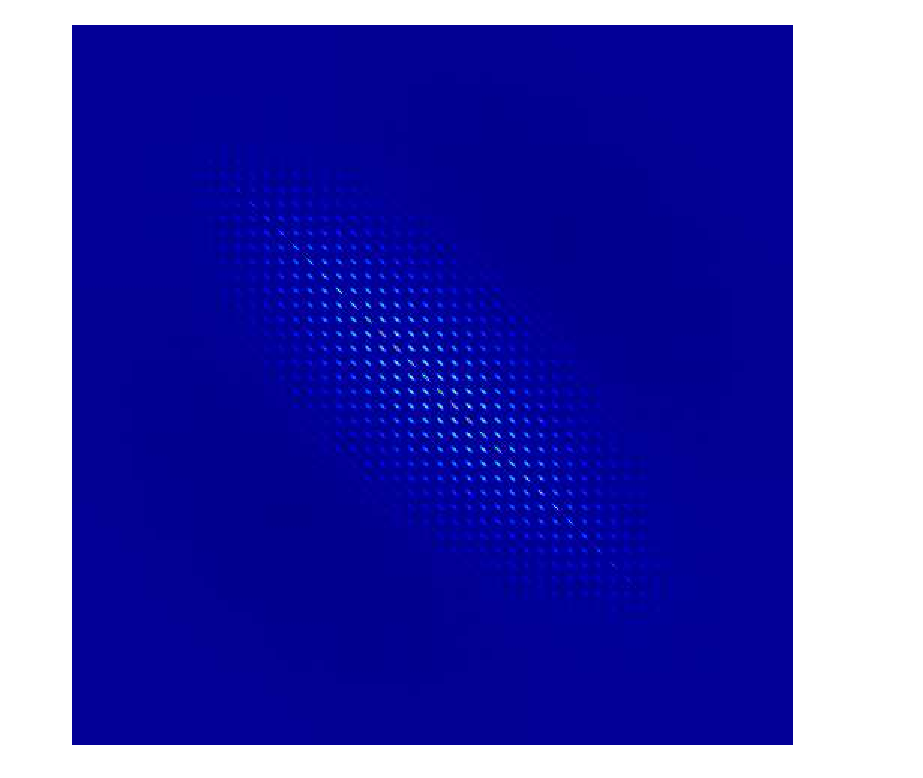
\includegraphics[width=0.2\linewidth]{figures/prior/outfile_drop2_cropped.pdf}} } &
                       			{ 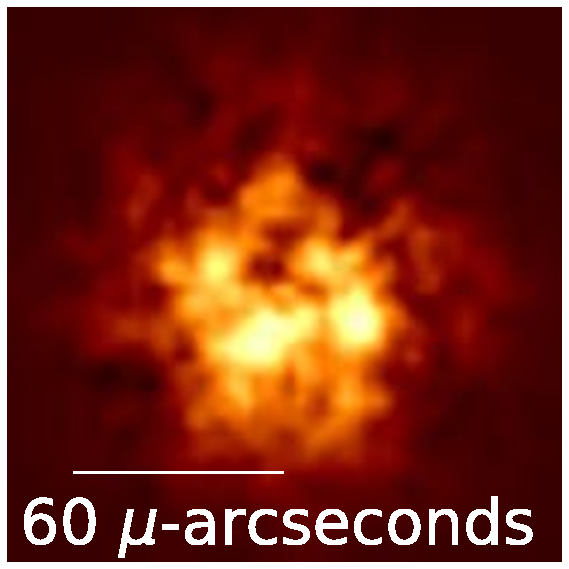
\includegraphics[width=0.2\linewidth]{figures/prior/newfiles/sampfig_drop2_1_scale2.pdf}} 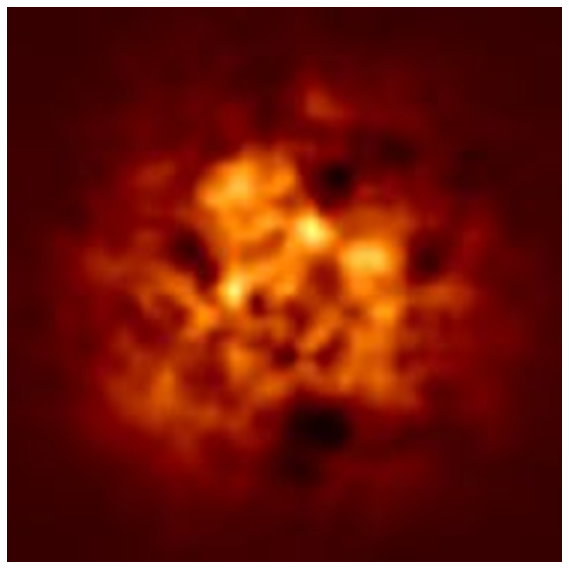
\includegraphics[width=0.2\linewidth]{figures/prior/newfiles/sampfig_drop2_4.pdf} 
                       			\multirow{3}{*}[.6in]{ 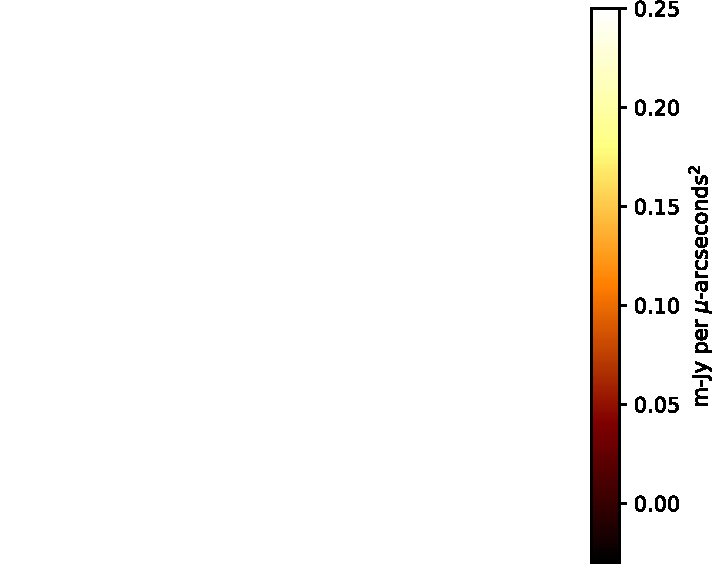
\includegraphics[width=0.155\linewidth]{figures/prior/newfiles/sampfig_drop2_1_cbar.pdf} }
                                \\
                       			&\vspace{-.1in}&\\
                       			\multirow{1}{*}[.6in]{ \rotatebox[origin=t]{90}{\large{\textsf{a = 3}} }} & 
                       			{{ 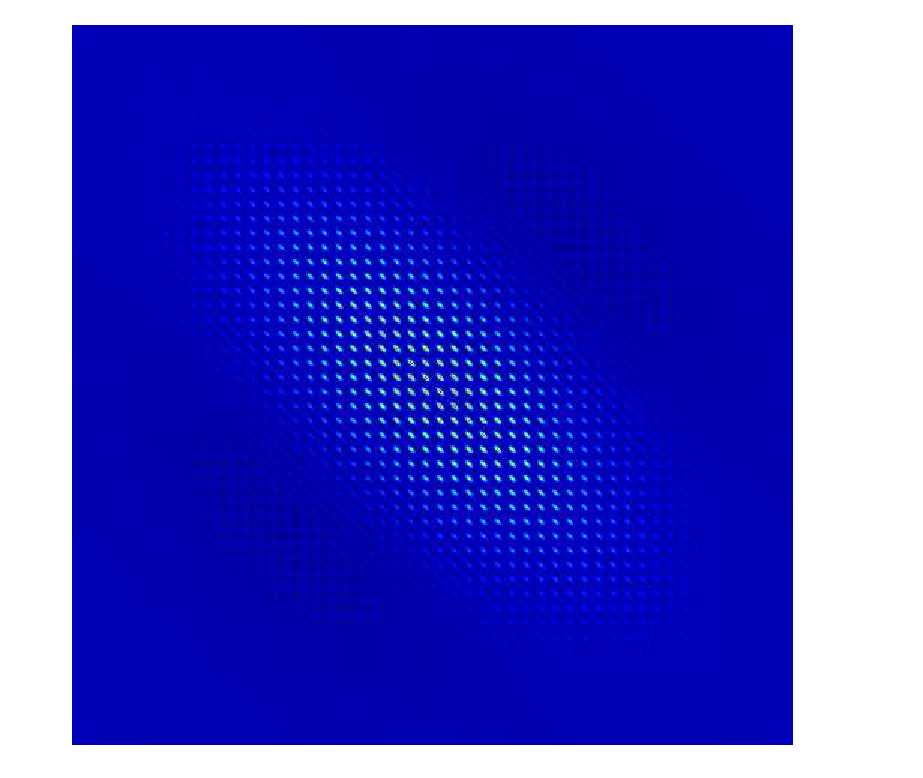
\includegraphics[height=0.2\linewidth]{figures/prior/outfile_drop3_cropped.pdf}} } &
                       			{ 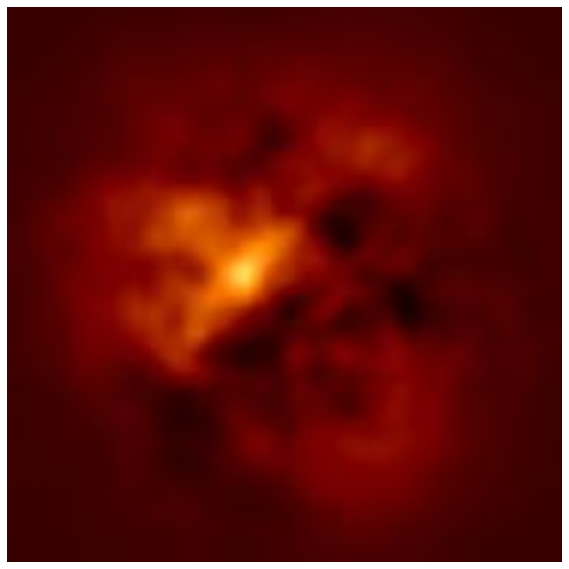
\includegraphics[height=0.2\linewidth]{figures/prior/newfiles/sampfig_drop3_2.pdf}} 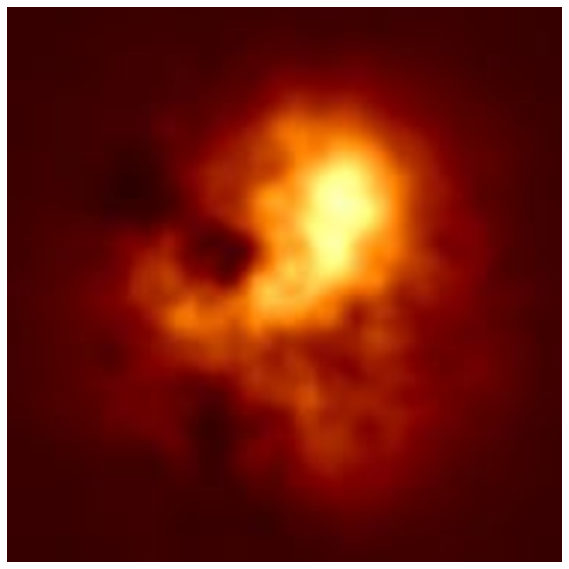
\includegraphics[height=0.2\linewidth]{figures/prior/newfiles/sampfig_drop3_3.pdf}  
                       			\hspace{.65in}
                       			%\multirow{3}{*}[.6in]{ 
\includegraphics[width=0.18\linewidth]{figures/prior/newfiles/placeholder.pdf} }
                       			\\
                       			&\vspace{-.1in}& \\
                       			\multirow{1}{*}[.6in]{ \rotatebox[origin=t]{90}{\large{\textsf{a = 4}} }} & 
                       			{{ 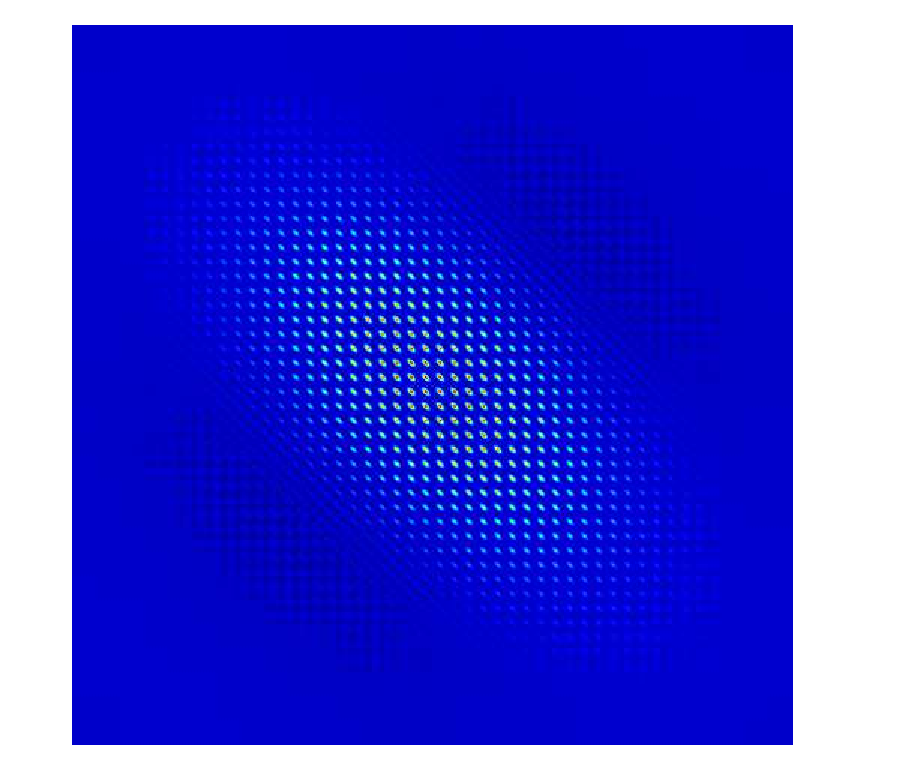
\includegraphics[height=0.2\linewidth]{figures/prior/outfile_drop4_cropped.pdf}} } &
                       			{ 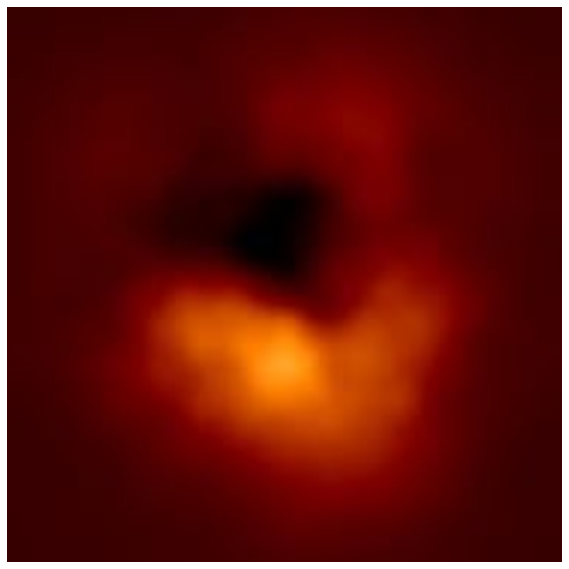
\includegraphics[height=0.2\linewidth]{figures/prior/newfiles/sampfig_drop4_1.pdf}} 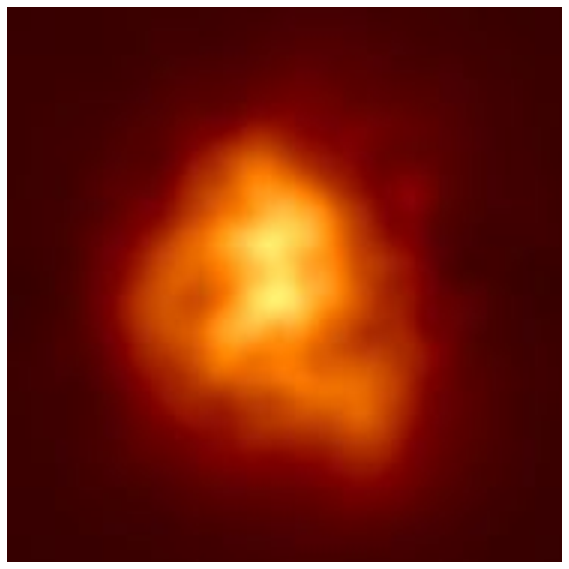
\includegraphics[height=0.2\linewidth]{figures/prior/newfiles/sampfig_drop4_2.pdf}                        			
                       			\hspace{.65in}
                       			%\multirow{3}{*}[.6in]{ 
\includegraphics[width=0.18\linewidth]{figures/prior/newfiles/placeholder.pdf} } 
                       			\\            	
                       		\end{tabular}
                       		\caption{\footnotesize{{\bf Gaussian Image Prior:} The covariance matrix constructed for $a=2,3,4$ along with image samples from the prior  $\mathcal{N}_x(\mu, \Lambda)$. The image samples have a field of view of 160 $\mu$-arcseconds. Notice that as $a$ increases, the sampled images appear smoother (i.e., the prior encourages smoother structure). In these examples $\mu$ is a 2D Gaussian image with standard deviation of 75 $\mu$-arcseconds. and $c=0.5$. 
                       			}}
                       			\label{fig:priorsamples}
\end{center}
\vspace{-.2in}
\end{figure}

\begin{figure*}[h!]
	\vspace{-.0in}
	\setlength{\tabcolsep}{1pt}
	\begin{center}
		\begin{tabular}{ c  c  | c  c  c c  }
			%\hline
			 \hspace*{-1.0cm}  
             \multirow{4}{*}[-0in]{ \rotatebox[origin=t]{0}{ {\vspace*{1in} 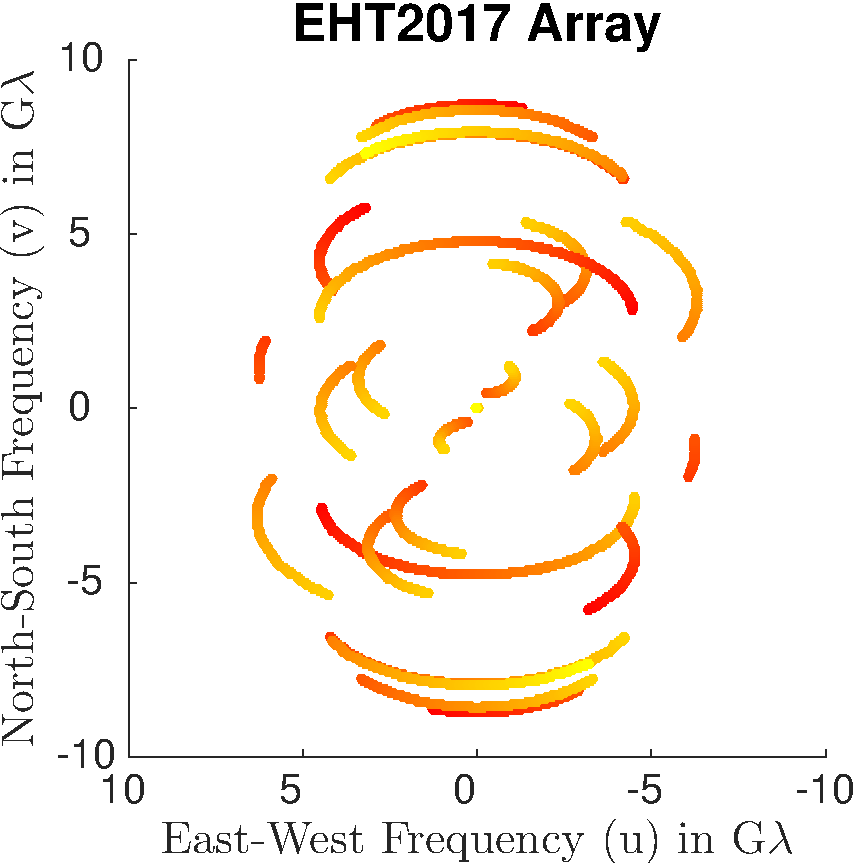
\includegraphics[trim=0cm 0 0 -4cm,height=.43\linewidth]{figures/uvcoverage/uv_eht2017_2.pdf}}
			 		\qquad  }}
			 &  \hspace{-0.7cm}  \large{\textsf{Truth}}   & &  \large{\textsf{a = 2}} & \large{\textsf{a = 5}}  &  \large{\textsf{a = 10}}    \\
			&  \hspace{-0.5cm} {{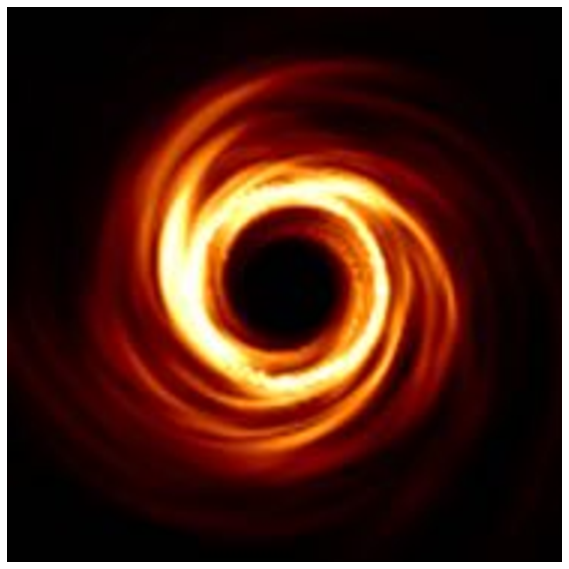
\includegraphics[height=.13\linewidth]{figures/singleimage/visibilities/hotakaframe3.pdf}} } &
			\multirow{1}{*}[0.82in]{ \rotatebox[origin=t]{90}{ \small{\textsf{Gauss. Recon.}} }}
			&
			{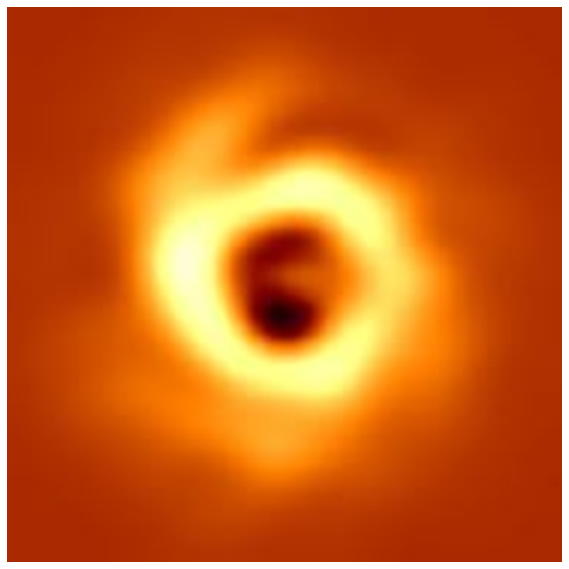
\includegraphics[height=.13\linewidth]{figures/singleimage/visibilities/img_powerdropoff_2.pdf}} &
			{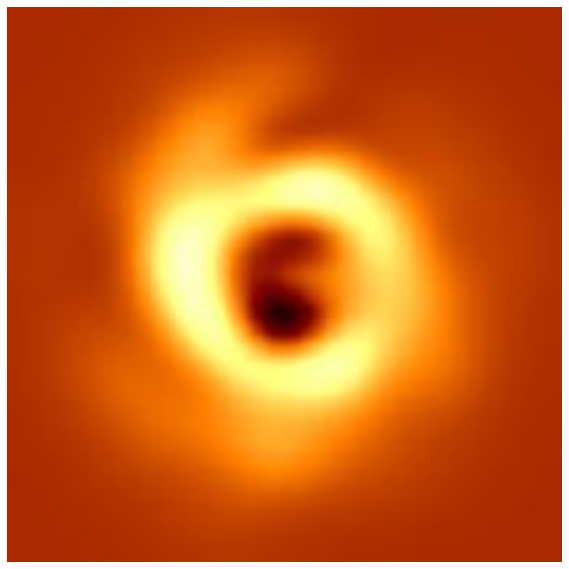
\includegraphics[height=.13\linewidth]{figures/singleimage/visibilities/img_powerdropoff_5.pdf}} 
			&
			{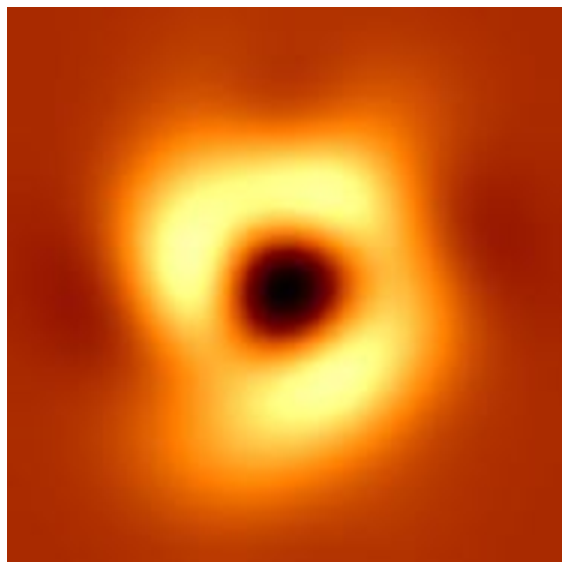
\includegraphics[height=.13\linewidth]{figures/singleimage/visibilities/img_powerdropoff_10.pdf}} 
			\\
			& \vspace{-.0in}  \hspace{-0.8cm} \large{\textsf{MEM \& TV}}  & &  \multicolumn{3}{c}{ 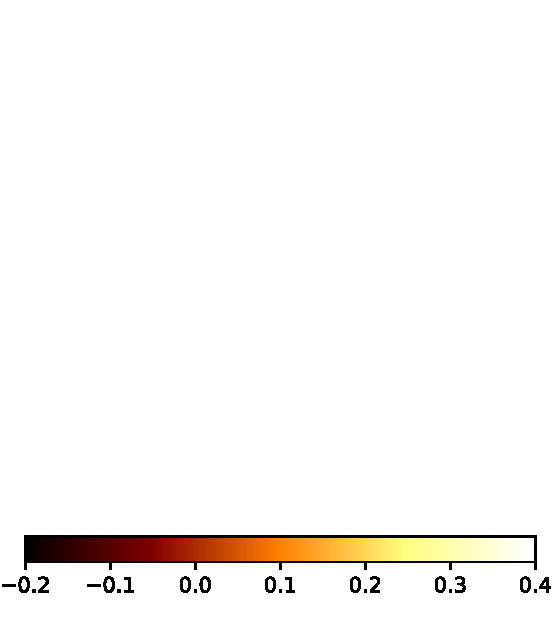
\includegraphics[width=.25\linewidth]{figures/cbar/horizontal_cbar_-2to4_r2.pdf} }
			\\
			%& \vspace{-.15in}  \hspace{-0.8cm} \large{\textsf{MEM \& TV}}  & & & &       \\
			&\hspace{-0.5cm} {{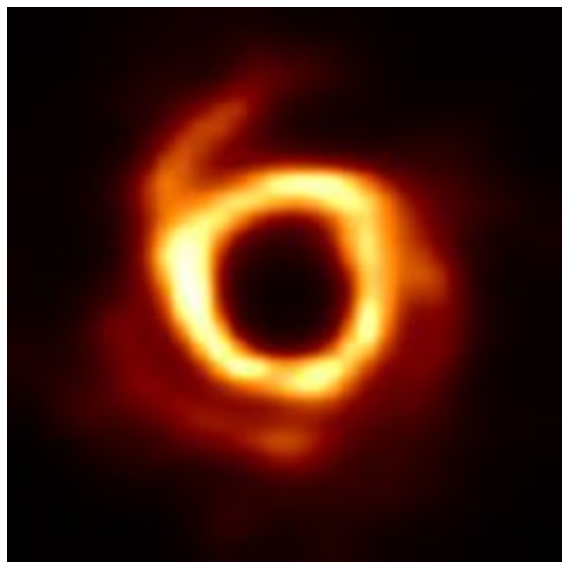
\includegraphics[height=.13\linewidth]{figures/singleimage/visibilities/img_maxen.pdf}} } &
			\multirow{1}{*}[0.82in]{ \rotatebox[origin=t]{90}{ \small{\textsf{Clipped Recon.}} }}
			&
			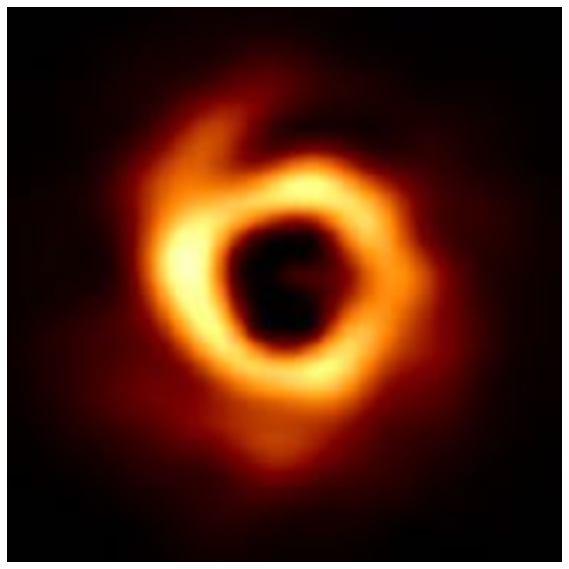
\includegraphics[height=.13\linewidth]{figures/singleimage/visibilities/imgClip_powerdropoff_2.pdf} &
			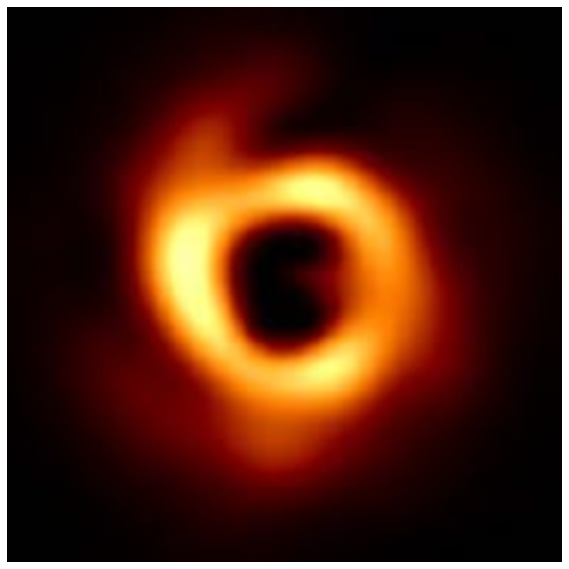
\includegraphics[height=.13\linewidth]{figures/singleimage/visibilities/imgClip_powerdropoff_5.pdf} &
			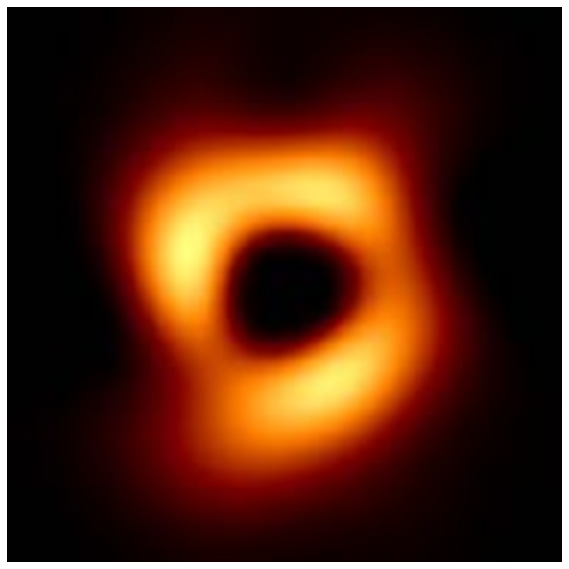
\includegraphics[height=.13\linewidth]{figures/singleimage/visibilities/imgClip_powerdropoff_10.pdf} 
			\\
			& \vspace{-.0in} \hspace{-.8cm} \large{\textsf{CHIRP}}  & &  \multicolumn{3}{c}{ 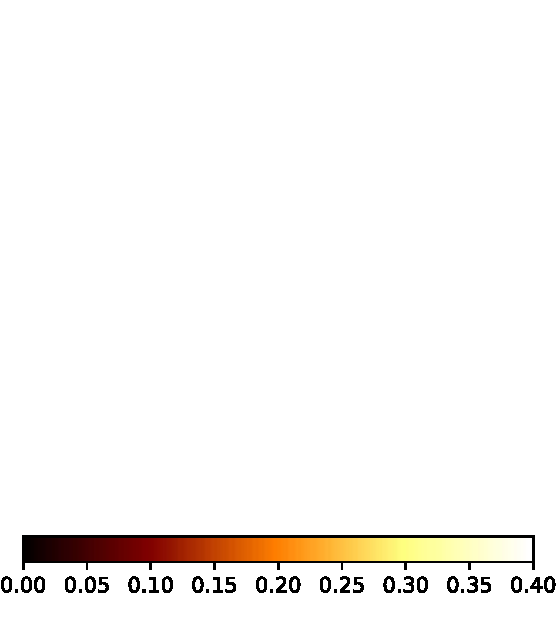
\includegraphics[width=.25\linewidth]{figures/cbar/horizontal_cbar_0to4_r2.pdf} }
			\\ 
			%& \vspace{-.15in} \hspace{-.8cm} \large{\textsf{CHIRP}}   & & & &     \\
			&\hspace{-0.5cm} {{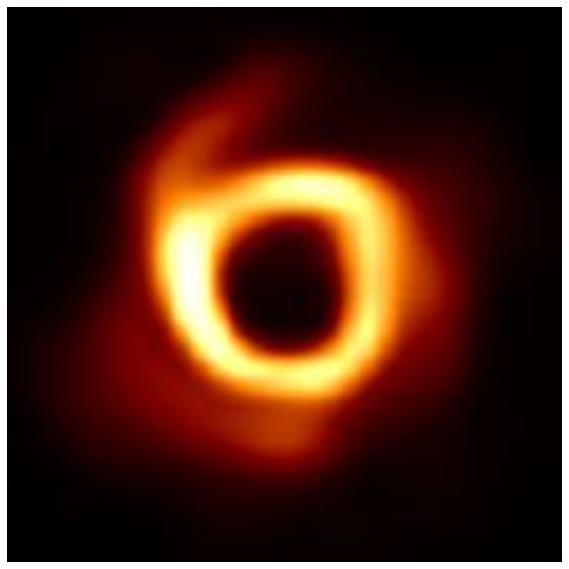
\includegraphics[width=.13\linewidth,trim=0.0cm -1.5cm 0.0cm 0.0cm]{figures/singleimage/visibilities/hotakaframe_chirp.pdf}} \vspace{0.04cm} } &
			\multirow{1}{*}[1.05in]{ \rotatebox[origin=t]{90}{ \small{\textsf{Diagonal Std. Dev. }} }}
			&
			\hspace{-.1in} 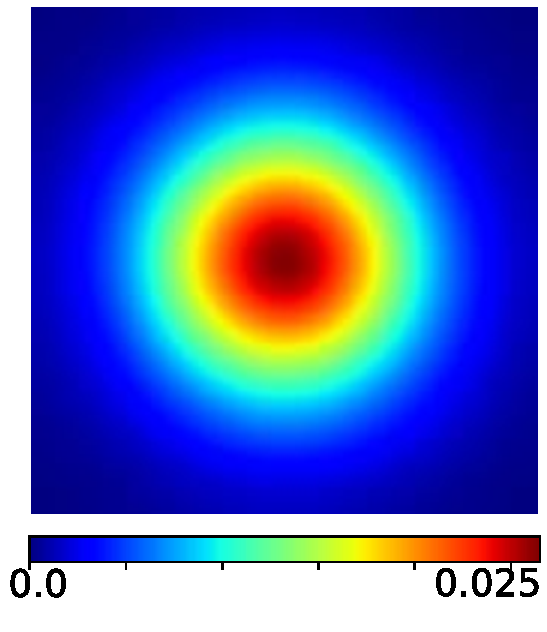
\includegraphics[width=.138\linewidth]{figures/singleimage/visibilities/covImg_powerdropoff_2_r2.pdf} &
			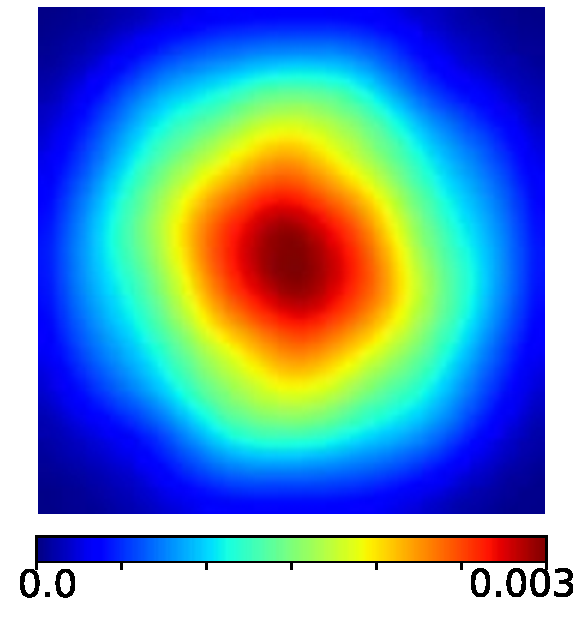
\includegraphics[width=.148\linewidth]{figures/singleimage/visibilities/covImg_powerdropoff_5_r2.pdf} 
			&\hspace{-.1in}
			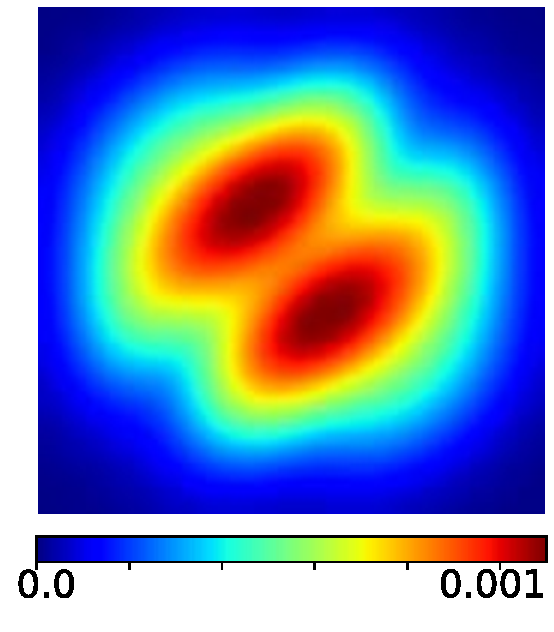
\includegraphics[height=.145\linewidth]{figures/singleimage/visibilities/covImg_powerdropoff_10_r2.pdf} 
		\end{tabular}
		\caption{{\bf Static Imaging Comparison:} Results of static imaging using a multivariate Gaussian prior ( \textsf{a} = 2, 5, 10) compared to state-of-the-art reconstruction methods using MEM \& TV regularizers~\cite{andrew} as well as patch-based regularizers (CHIRP)~\cite{bouman2016computational}. All images are shown with a field of view of 160 $\mu$-arcseconds. Data is generated using a static image with the uv-coverage of the EHT2017 array shown on the left (see Section~\ref{sec:results}). The uv-coverage is colored by time, as indicated by the colorbar in Figure~\ref{fig:uvcov2}. Note however that in this static imaging case the time of measurements is not relevant. Although the previous algorithms (MEM \& TV and CHIRP) both produce better results, the Gaussian reconstruction is able to correctly get the broad structure of the underlying image. Since we do not impose positivity, negative values are reconstructed. However, by clipping the resulting image we can see that the result aligns well with the true static image. The Gaussian prior model also allows us to easily estimate our reconstructed image uncertainty. We visualize the diagonal entries of the posterior covariance matrix as the reshaped standard deviation image. Note that as the smoothness parameter \textsf{a} is increased, the per-pixel standard deviation becomes smaller, but the structure of the standard deviation deviates from what was specified in the prior (recall $\bLambda$ is scaled by $\bmu$, which we have specified as a 2D Gaussian in this work). For large \textsf{a} the uncertainty is shown to be primarily in the diagonal north-west to south-east direction, due to the lack of spatial frequencies sampled by the telescope array in this direction. To avoid approximations and best show the recovered posterior covariance matrices, atmospheric error has not been included in the data used to recover these images. The scaling of the colormaps is in mili-Jansky per squared $\mu$-arcsecond. } 
		\label{fig:staticimaging}
		%-.2, .4
		%0, .4
	\end{center}
	\vspace{-.2in}
\end{figure*}



\vspace{-.2in}
\subsection{Multivariate Gaussian Image Prior}
\label{sec:gauss_prior}

A prior distribution on $\im$ constrains the space of possible solutions during inference, and can be defined in a variety of ways.
%There are many ways that a prior distribution on $\im$ can be defined. 
For instance, maximum entropy, sparsity, and patch priors have been all used previously for VLBI imaging~\cite{andrew,kazu,bouman2016computational, rusenimaging}.
%Priors that have been used previously in VLBI imaging include maximum entropy, sparsity, and patch priors. 
In this work we instead choose to define the underlying image, $\im$, as being a sample from the distribution $\mathcal{N}_{\im}(\bmu, \bLambda)$. This choice leads to less sharp image reconstructions compared to richer priors, %is less powerful 
%expressive
%than some of the other image priors in reconstructing a sharp image, 
%but its simple expression 
%comes with the advantage of allowing 
%allows for a better theoretical understanding of our solutions, which proves especially valuable when propagating uncertainties in dynamical imaging (refer to Section~\ref{sec:dynamic_inference}). 
but its simplicity allows for a cleaner understanding of our solutions. This proves especially valuable in propagating uncertainties during dynamic imaging (refer to Section~\ref{sec:dynamic_inference}). 
%is less expressive
%allows for a better theoretical understanding of our solutions that BLAH BLAH BLAH.  

%Image regularizers that enforce spatial smoothness can often be described with a multivariate Gaussian image prior. 
%For instance, the common squared total variation regularizer can be expressed by writing the image covariance, $\bLambda$, in terms of  the $ 2 \npix^4 \times \npix^4$ gradient matrix, $\bm{G}$: $\bLambda \propto \left[ \bm{G}^T \bm{G} \right]^{-1}$.

Studies have shown that the average power spectrum of an image often falls with the inverse of spatial frequency in the form $1/(u^2 + v^2)^{a/2}$, where $a$ is a value that specifies the smoothness of the image~\cite{torralba2003statistics}. 
%$1/f^a$. %(Burton and Moorhead 1987, Field 1987, 1994, Tolhurst et al 1992) http://web.mit.edu/torralba/www/ne3302.pdf
As the amplitude of a spatial frequency is linearly related to the image itself, this statistical property can also be enforced by specifying the covariance in a prior distribution. Specifically, 
%\begin{align}
%\bLambda'  =  &  \bm{W}^{*T}  \mbox{diag} \left[ \frac{1}{ %(\bm{u}^2 + \bm{v}^2)^{a/2} } \right]  \bm{W} 
%\end{align}
\begin{align}
& \hspace{.5in} \bLambda'  =    \bm{W}^{*T}  \mbox{diag} \left[ \bm{b}  \right]  \bm{W}  \\ 
b[i] = & \begin{cases} 
({u[i]}^2 + {v[i]}^2)^{-a/2}  & {u[i]}^2 + {v[i]}^2 > 0 \\
\epsilon & {u[i]}^2 + {v[i]}^2  = 0 \\
\end{cases}
\end{align}
\noindent{for DFT matrix $\bm{W}$ of size $M^2 \times M^2$ %and vector $\bm{b}$ of size $M^2$ 
for an $M\times M$ pixel image and a small positive value, $\epsilon$. Each row of $\bm{W}$ and $\bm{b}$ %is comprised of $\vecFTmtx(u,v)$ (see Section BLAH), and 
	corresponds to a $(u,v)$ coordinate in the 2D grid of frequencies, \{ $S \times S$ \}, for }
\begin{align}
%UV &= S \times S = \{ (u,v) | u \in S, v \in S \} \\
S &= \left\{ \frac{m-M/2}{FOV} \right\}, m\in \mathbb{Z}: m \in [0,M-1],
\end{align}
where $FOV$ is the image's field of view in radians.
To specify the variance of each pixel and help encourage positivity, we modify the amplitude of the covariance by left and right multiplying by ${c \cdot \mbox{diag}[\bmu ]} $:
\begin{align}
\bLambda = c^2 \mbox{diag}[\bmu ]^T \bLambda' \hspace{0.01in} \mbox{diag}[\bmu ] 
\end{align}
\noindent{A $c$ value of 1/3 implies that 99\% of flux values sampled from $\mathcal{N}_x(\bmu, \bLambda)$ will be positive. In this work we have chosen $\mu$ to be a circular Gaussian with a standard deviation of 40-50\% of the reconstructed FOV to encourage most of the flux to stay near the center of the image and away from the edges. Figure~\ref{fig:priorsamples} shows the covariance matrix constructed for $a=2,3,4$ along with images sampled from the prior  $\mathcal{N}_x(\bmu, \bLambda)$. Notice that as $a$ increases, the sampled images are smoother. Thus, $a$ provides the ability to tune the desired smoothness of the inferred images. 
}

%THIS DOESNT BELONG HERE!!!
%In Section BLAH we explain how this image prior can be introduced into the estimation of each $x_t$. Introducing the prior into the estimate of each image helps to further constrain the images in this very ill-posed setting. 


\subsection{Inference}
\label{sec:static_inf}

%As a Gaussian distribution is a conjugate prior for a Gaussian likelihood, the posterior distribution 

Our goal is to find the most likely image, $\im$, that describes the data products we have observed, $\meas$. A maximum a posteriori (MAP) solution is found by maximizing the log-posterior from Equation~\ref{eq:bayes}:
\begin{align}
\hat{\im}  = \argmax_{\im} & \log p(\im|\meas) \\
\notag =  \argmin_{\im}  &\left[ (f(\im)-\meas)^T \bR^{-1} (f(\im)-\meas) \right. \\
& \left. + (\im-\bmu)^T \bLambda^{-1} (\im-\bmu) \right] .
\end{align}

Note the similarities of this equation's structure to that of previous static imaging methods in Equation~\ref{eq:setup} and~\ref{eq:chi2}. 
Although the hyperparameter $\gamma$ is no longer explicit, the scaling of $\bLambda$ acts like this hyperparameter and balances influence of the measured data with influence of the prior.
%used in many VLBI imaging frameworks.

%\subsection{Data Likelihood - change from likelihood}


\vspace{0.1in}
\subsubsection{Linear Measurements}


As explained in Section~\ref{sec:dataproducts}, $f(\im)$ is linear when $\meas$ is composed solely of calibrated complex visibilities with no %remaining
atmospheric error.
In this case -- when $f(\im) = \FTmtx \im$ --
%with corresponding Gaussian noise of variance, $\bm{\sigma}^2$  (i.e. no atmospheric error), 
a closed-form solution of $\hat{\im}$ can be found %. 
%In the case that $f(\im) = \FTmtx \im$ is a linear function of $\im$,a closed-form solution of $\hat{x}$ can be found. 
%In this situation, $\im$ can be solved 
through traditional Weiner filtering. Specifically, we can compute the most likely estimate of each $\im$ as: 
% Equation~\ref{eq:map}:
\begin{align}
\hat{\im} &=  \bmu  + \bLambda {\bf F}^T ( \bR + \FTmtx \bLambda \FTmtx^{T} )^{-1} (  \meas -  \FTmtx \bmu ) .
\label{eq:map}
\end{align}
\noindent{
	%Refer to the supplemental material for details of this derivation. 
	In the limit of having no prior information about the underlying image $\im$, e.g.,  $\bLambda = \lim_{\lambda \to\infty} \lambda \mathds{1}$ for identity matrix $\mathds{1}$, this MAP solution reduces to $\hat{\im} =  \FTmtx^{+} \meas$. In other words, in the absence of prior image assumptions, the noise on each measurement, $\bR$, is no longer relevant and the reconstructed image is simply obtained by inverting $\meas = \FTmtx \im$.
	This is very similar to reconstructing the ``dirty image''~\cite{taylor1999synthesis}.
	
%When $\meas$ are sparse visibilities, although $\FTmtx^{-1}$ is undefined, since $\FTmtx \FTmtx^{*T} = \mathds{1}$, $\hat{\im} =  \FTmtx^{-1} \meas$ is very similar to reconstructing the ``dirty image''~\cite{taylor1999synthesis}.

%evaluating, inspecting

The same solution can also be obtained by evaluating %and inspecting 
the posterior distribution. 
With a linear measurement function, $f(\im)$, the proposed Gaussian formulation leads to a closed-form expression for the posterior. In particular, 
\begin{align}
p(\im|\meas) & = \mathcal{N}_{\im} (\hat{\im}, \bm{C} ). 
\end{align}
for covariance matrix
%\noindent{The mean of this posterior distribution is equivalent to the MAP estimate obtained through Weiner Filtering.}
%Our proposed Gaussian formulation not only facilitates easily computing the MAP estimate, but also the uncertainty in the estimated $\hat{\im}$:
\begin{align}
\bm{C} = \bLambda - \bLambda \FTmtx^T ( \bR + \FTmtx \bLambda \FTmtx^T )^{-1} \FTmtx \bLambda .
\end{align}
\noindent Estimating uncertainty with the covariance matrix is useful in understanding what regions of the reconstructed image we trust. This becomes especially helpful when propagating information in dynamical imaging, as will be demonstrated in Figure~\ref{fig:propinfo}. 




\vspace{0.1in}
\subsubsection{Non-linear Measurements}
%When the data products in $\meas$ are invariant to atmospheric noise, $f(\im)$ is a non-linear function of $\im$ and a closed-form solution does not exist. 
When $f(\im)$ is a non-linear function of $\im$, as is the case when the data products in $\meas$ are invariant to atmospheric noise, a closed-form solution does not exist. 
%of atmospheric noise, large phase errors are added to the complex visibility measurements. However, these phase errors are incorporated in a way that preserves closure phase (refer to Section BLAH). In order to handle this additional phase error, without having to explicitly model the errors as latent variables, we can change the measurement function, $f(.)$, to one that is invariant to atmospheric inhomogeneity.
%A measurement function, $f(.)$, which extracts the bispectrum, visibility amplitude, or closure phase would be invariant to this atmospheric inhomogeneity. However, it comes at the expense of being a non-linear function of the image, $x$. 
However, to solve for the optimal $\im$ we linearize $f(\im)$ to obtain an approximate solution, $\hat{\im}$. Using a first order Taylor series expansion approximation around $\tilde{\im}$, we approximate the data likelihood as
\begin{align}
p(\meas|\im) = \mathcal{N}_{\meas}(f(\im),\bR) \approx \mathcal{N}_{\meas} \left( f( \tilde{\im} ) +  \dot{\FTmtx} (\im - \tilde{\im} )  , \bR \right) , 
\end{align}
\noindent{ for $\dot{\FTmtx} = \left. \frac{df(\im)}{d \im} \right| _{\tilde{\im} }$. Using this approximation, % we solve for 
	the optimal $\hat{\im}$ is}
\begin{align}
\hat{\im} &=  \bmu  + \bLambda \dot{\FTmtx}^T ( \bR + \dot{\FTmtx} \bLambda \dot{\FTmtx}^{T} )^{-1} (  y  - f(\tilde{\im}) +  \dot{\FTmtx} (\tilde{\im}-\bmu) ) .
\label{eq:approxoptimal}
\end{align}

To further improve the solution, we solve Equation~\ref{eq:approxoptimal} iteratively by updating  $\hat{\im}$ and setting $\tilde{\im} = \hat{\im} $ until convergence.
%By iteratively solving for Equation~\ref{eq:approxoptimal} and setting $\tilde{\im} = \hat{\im} $, we can improve our estimated image reconstruction, $\hat{\im}$. 
Note that in the case that $f(\im)$ is linear, $\dot{\FTmtx} = \FTmtx$ and Equation~\ref{eq:approxoptimal} reduces to Equation~\ref{eq:map}. We compare results of this reconstruction method to other state-of-the-art methods for a static source in Figure~\ref{fig:staticimaging}. Figure~\ref{fig:staticimaging} demonstrates that, although this approach does not outperform other state-of-the-art static imaging methods, reasonable results are achieved despite a simpler image regularizer and optimization procedure. This simpler approach will become useful in developing a dynamic imaging approach. 


\vspace{-.05in}
\section{Method}
\label{section:Method}
\vspace{-.05in}

\begin{figure}[b]
	\vspace{-.0in}
	\centering
	%\fcolorbox{bordercolor}{paddingcolor}{image}
	\fcolorbox{red}{red}{\includegraphics[width=0.2\linewidth]{ex2.png}}
	\fcolorbox{green}{green}{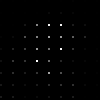
\includegraphics[width=0.2\linewidth]{deltaPulses_ex2_big.png}}
	\fcolorbox{cyan}{cyan}{
\includegraphics[width=0.2\linewidth]{rectPulses_ex2.png}}
	\fcolorbox{blue}{blue}{
\includegraphics[width=0.2\linewidth]{trianglePulses_ex2.png}}
	
	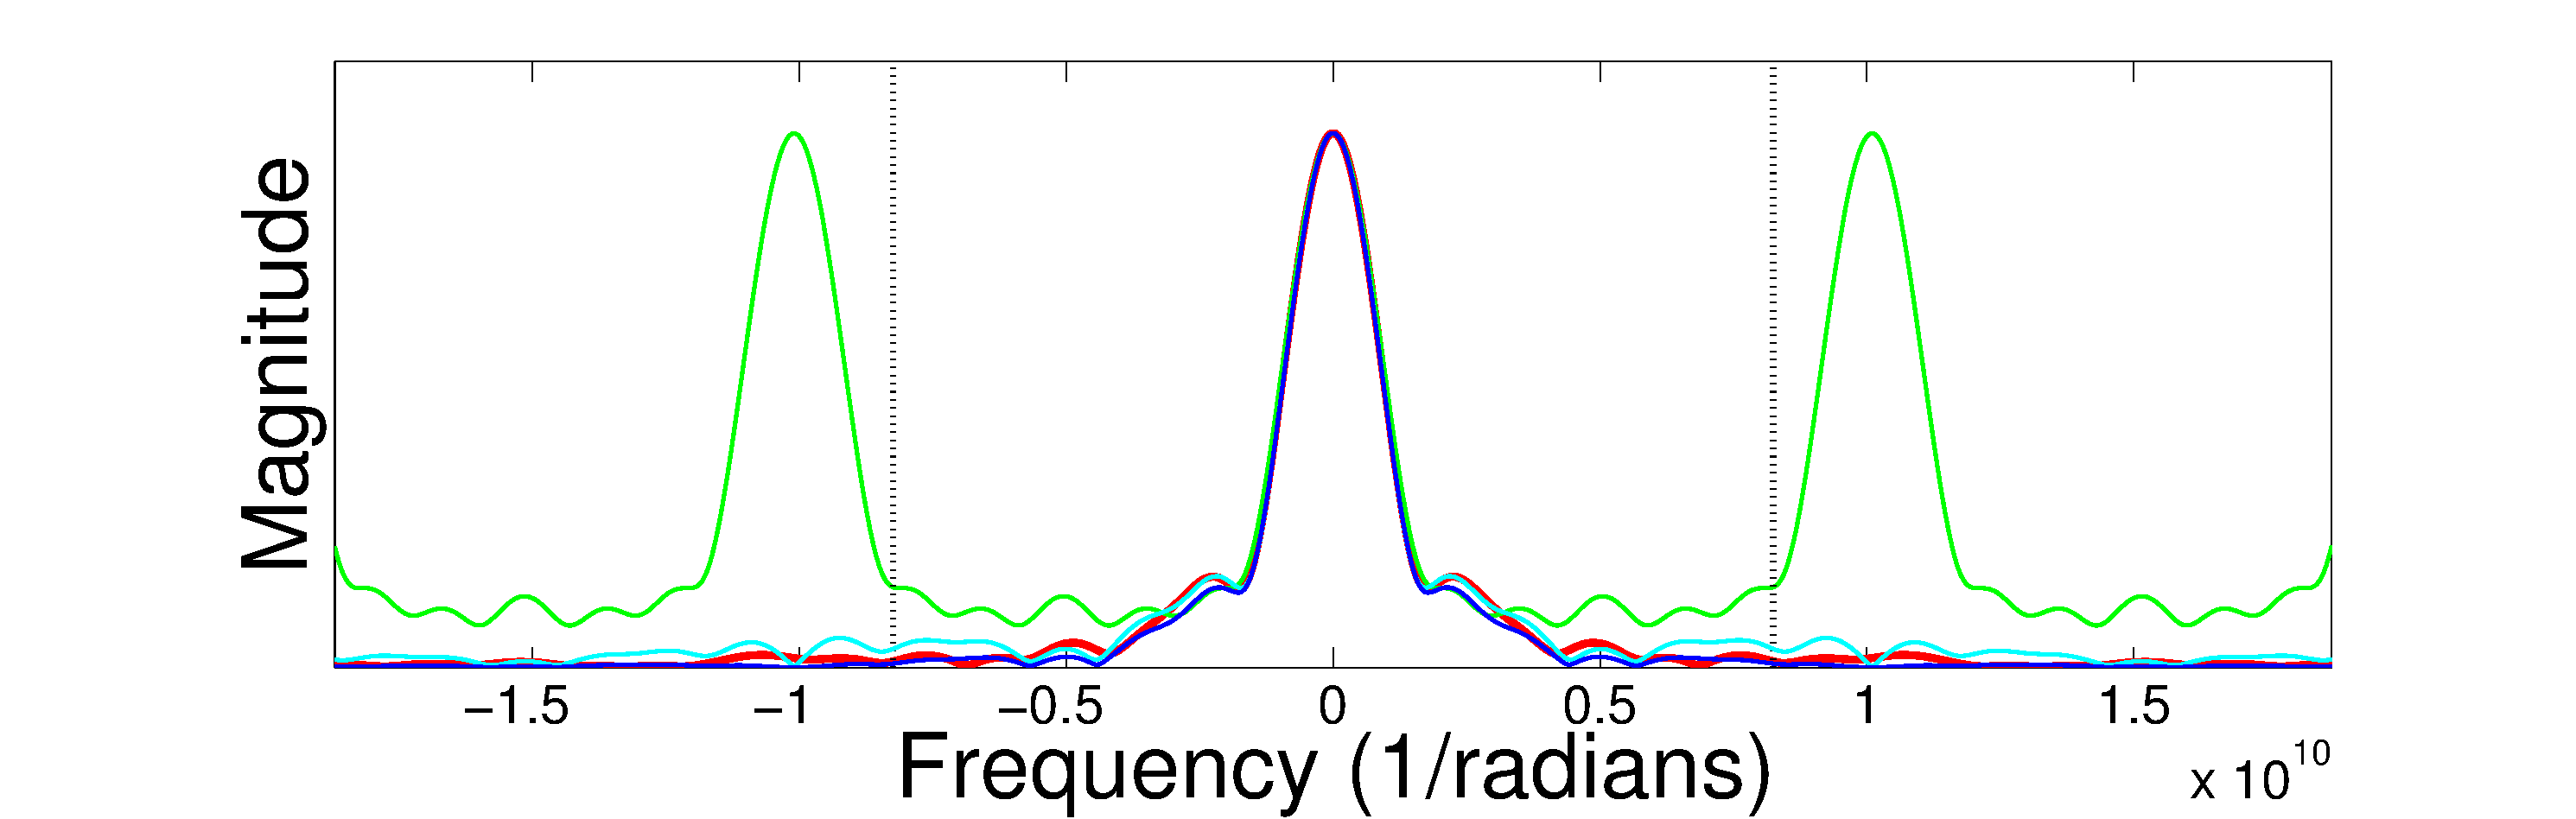
\includegraphics[width=0.95\linewidth]{freqfig_9pulses_wrect_zoom_ex2_2.pdf}
	\caption{\footnotesize{Accurately modeling the frequencies of an image is crucial for fitting VLBI measurements during image reconstruction. Here we show, that with the same number of parameters, we can much more accurately model the true frequency distribution. A slice of frequencies for the true image is shown in red. Overlayed we show the effect of using the traditional discretized imaging model (green), and our improved model for rectangle (cyan) and triangle (blue) pulses. The dotted lines denote the frequency range sampled in Fig~\ref{fig:uvcov}b. Representing an image in this way reduces modeling errors for higher frequencies during image reconstruction.}}
	\label{fig:pulses}
\end{figure}

\begin{figure*}[!t]
	\vspace{-.2in}
	% ensure that we have normalsize text
	\normalsize
	% Store the current equation number.
	%		\setcounter{MYtempeqncnt}{\value{equation}}
	% Set the equation number to one less than the one
	% desired for the first equation here.
	% The value here will have to changed if equations
	% are added or removed prior to the place these
	% equations are referenced in the main text.
	\setcounter{equation}{5}
	%\hrulefill
	{\small
		\begin{align}
		\notag \Gamma(u,v) &\approx \int_{- \infty}^{\infty}\int_{- \infty}^{\infty} {e^{-i 2 \pi  (u\ell + vm) }} \sum_{i=0}^{N_\ell-1}\sum_{j=0}^{N_m-1} x[i,j] 
		h \left(\ell- \left( \Delta_{\ell}i + \frac{\Delta_{\ell}}{2}  -\frac{FOV_\ell}{2} \right),m- \left( \Delta_mj + \frac{\Delta_m}{2} -\frac{FOV_m}{2} \right) \right)  d\ell dm  
		\\ &=  \sum_{i=0}^{N_\ell-1}{\sum_{j=0}^{N_m-1}  x[i,j] e^{-i 2 \pi \left(u  \left( \Delta_{\ell}i + \frac{\Delta_{\ell}}{2} + a_\ell \right) + v \left( \Delta_mj + \frac{\Delta_m}{2} + a_m \right)  \right)} H(u, v)} = A {\bf x} = \left( A^{\Re} + i A^{\Im} \right) {\bf x}
		\label{eq:formodel}
		\end{align} 
	}
	\vspace{-.25in}
	% Restore the current equation number.
	%		\setcounter{equation}{\value{MYtempeqncnt}}
	% IEEE uses as a separator
	\hrulefill
	% The spacer can be tweaked to stop underfull vboxes.
\end{figure*}


%In this section we describe our proposed algorithm for reconstructing an image using bispectrum measurements.
% obtained using a VLBI telescope array. 
Reconstructing an image using bispectrum measurements is an ill-posed problem, and as such there are an infinite number of possible images that explain the data~\cite{rusenimaging}. 
%To find an optimal solution, we must rely on prior assumptions about the ``visual" universe. 
The challenge is to find an explanation that respects our prior assumptions about the ``visual" universe
%looks  ``good" under some measure
while still satisfying the observed data. 
%Note that this problem differs from traditional sparse spectral reconstruction methods (e.g MRI, CT) due to the large atmospheric phase errors. 



%For every two telescopes in an $N$ telescope array we measure a single complex Fourier component of $I_{\lambda}$. Assuming that the atmosphere does not affect our measurements, this means that we have constraints on $ \frac{N(N-1)}{2} $ of the image's frequency components. The task of reconstructing an image from just these components is highly under-constrained since there are infinite possibilities for what values could fill the remaining frequency components. Therefore, to find an optimal solution, we must rely on our prior assumptions about the ``visual" universe. Using a prior image model narrows our search space substantially and helps us find a reasonable looking image that also fits the the measurements~\cite{felli1989very}. 


\subsection{Continuous Image Representation}


The image that we wish to recover, $I_{\lambda}(\ell,m)$, is defined over the continuous space of angular coordinates $l$ and $m$. 
%However, computers require that we work with discrete elements.  
%rather than discretizing the measurements, 
%\katie{To account for the expected resolution of the instrument,} 
Many algorithms assume a discretized image of point sources during reconstruction 
%and subsequently blur the final image to account for the expected instrumental resolution
~\cite{taylor1999synthesis}. This discretization introduces errors during the reconstruction optimization, especially in fitting the higher frequency visibilities.
Instead, we parameterize a continuous image using a discrete number of terms. 
{\it This parameterization not only allows us to model our emission with a continuous image, but it also reduces modeling errors during optimization. }
%{\it This parameterization not only allows us to reduce modeling error} by easily evaluating the likelihood of measuring a set of visibilities from an estimate of the continuous image during optimization. 

Since each measured complex visibility is approximated as the Fourier transform of $I_{\lambda}(\ell,m)$, a convenient parameterization of the image is to represent it as a discrete number of scaled and shifted continuous pulse functions, such as triangular pulses.
% that have an analytic Fourier transform. 
For a scene defined in the range $\ell \in [-\frac{F_\ell}{2}, \frac{F_\ell}{2}]$ and $m \in [-\frac{F_m}{2}, \frac{F_m}{2}]$,
%and is assumed to have zero flux density outside the field of view,
we parameterize our space into $N_\ell \times N_m$ scaled pulse functions, $h(l,m)$, centered around 

%\vspace{-.17in}

\begin{align}
 l &= i \Delta_{\ell} + \frac{\Delta_{\ell}}{2}  -\frac{F_\ell}{2} \hspace{0.26in} \mbox{for} \hspace{0.1 in} i = 0,...,N_\ell-1
 \label{eq:discrete1}
\\m &= j\Delta_m + \frac{\Delta_m}{2} -\frac{F_m}{2} \hspace{0.1in} \mbox{for} \hspace{0.1 in} j= 0,...,N_m-1
\label{eq:discrete2}
\end{align} 


\vspace{-.09in}
\noindent{for $\Delta_{\ell} = \frac{F_\ell}{N_\ell}$ and $\Delta_m = \frac{F_m}{N_m}$. Using Eq.~\ref{eq:discrete1} and~\ref{eq:discrete2} we can represent a continuous image as a discrete sum of shifted pulse functions scaled by $x[i,j]$. We refer to this image as $\hat{I}_{\lambda}({\bf x})$ for vectorized coefficients ${\bf x}$. 


%
%\begin{figure}[b]
%	\centering
%	%\fcolorbox{bordercolor}{paddingcolor}{image}
%	\fcolorbox{red}{red}{\includegraphics[width=0.2\linewidth]{images/newfigscvpr/pulses/ex2.png}}
%	\fcolorbox{green}{green}{\includegraphics[width=0.2\linewidth]{images/newfigscvpr/pulses/deltaPulses_ex3.png}}
%	\fcolorbox{cyan}{cyan}{
\includegraphics[width=0.2\linewidth]{images/newfigscvpr/pulses/rectPulses_ex2.png}}
%	\fcolorbox{blue}{blue}{\includegraphics[width=0.2\linewidth]{images/newfigscvpr/pulses/trianglePulses_ex3.png}}
%	
%	\includegraphics[width=0.95\linewidth]{images/newfigscvpr/pulses/freqfig_8pulses_wrect_zoom_ex3.eps}
%	\caption{\footnotesize{To accuratetly model an image's visibilities, we must write {\color{red} BLAH BLAH BLAH. TODO THIS CAPTION} Representing an image in this way reduces modeling errors during image reconstruction.}}
%	\label{fig:pulses}
%\end{figure}





%\begin{figure}[b]
%	\centering
%	%\fcolorbox{bordercolor}{paddingcolor}{image}
%	\fcolorbox{red}{red}{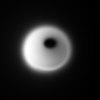
\includegraphics[width=0.2\linewidth]{images/newfigscvpr/newresults/blackhole40/blackhole40.png}}
%	\fcolorbox{green}{green}{\includegraphics[width=0.2\linewidth]{images/newfigscvpr/pulses/deltaPulses.png}}
%	\fcolorbox{cyan}{cyan}{\includegraphics[width=0.2\linewidth]{images/newfigscvpr/pulses/rectPulses.png}}
%	\fcolorbox{blue}{blue}{\includegraphics[width=0.2\linewidth]{images/newfigscvpr/pulses/trianglePulses.png}}
%	
%	\includegraphics[width=0.95\linewidth]{images/newfigscvpr/pulses/freqfig_8pulses_wrect_zoom.eps}
%	\caption{\footnotesize{To accuratetly model an image's visibilities, we must write {\color{red} BLAH BLAH BLAH. TODO THIS CAPTION} Representing an image in this way reduces modeling errors during image reconstruction.}}
%	\label{fig:pulses}
%\end{figure}

%
%   \begin{figure}[ht!]
%\centering
%  {\includegraphics[width=\linewidth]
%                   {images/forwardmodel/trianglePulse.eps}}                                               
%                    \caption{\footnotesize{An example of a continuous 1D image defined in terms of 1D triangle pulses. Pulses are shifted and scaled by a discrete set of values, $X[i]$. These shifted and scaled pulses are then summed together to make a single continuous image. In this example $X[i] = [1,2,3,1,1,4]$. Note how each point in the continuous image is a linear interpolation of its neighbors when using a triangle pulse. Representing an image in this way reduces modeling errors during image reconstruction. }}
% \label{fig:trianglePulse}
%\end{figure}

%\begin{align*}
%I_{\lambda}(\ell,m) \approx \sum_{i=0}^{N_{\ell}-1}{\sum_{j=0}^{N_m-1} X[i,j] h \left(l- \left( \Delta_{\ell}i + \frac{\Delta_{\ell}}{2} + a_{\ell} \right),m- \left( \Delta_mj + \frac{\Delta_m}{2} + a_m \right)\right) }
%\label{eq:discrete}
% \end{align*} 
 
 Due to the shift theorem~\cite{oppenheim1997signals}, plugging this image representation into the van Cittert-Zernike theorem (Eq.~\ref{eq:visibility}) results in a closed-form solution to the visibilities in terms of $H(u,v)$, the Fourier transform of $h(l,m)$, as seen in Eq.~\ref{eq:formodel}. Note that performing a continuous integration has been reduced to a linear matrix operation similar to a Discrete Time Fourier Transform (DTFT). 
 
 
In Figure~\ref{fig:pulses} we show that this representation allows us to approximates the true frequency components more accurately than a discretized set of point sources, especially for high frequencies.  
%In optimization, this formulation asks us to find the best set of coefficients $X[i,j]$ to explain $I_{\lambda}(\ell, m)$ under the assumed pulse model. 
Any pulse with a continuous closed-form Fourier transform can be used in this representation (e.g. rectangle, triangle, sinc, Gaussian). The chosen pulse places an implicit prior on the reconstruction. For instance, a sinc pulse with frequency and spacing $\Delta$ can reconstruct any signal with a bandwidth less than $\frac{\Delta}{2}$~\cite{oppenheim1997signals}. In this work we choose to use a triangle pulse with width $(2\Delta_\ell, 2\Delta_m)$ since this is equivalent to linearly interpolating between pulse centers and also simplifies 
%lends itself nicely to
non-negativity constraints. %(Figure~\ref{fig:trianglePulse}). 
Although we developed this image model for VLBI image reconstruction, it has potential applicability to a much more general class of imaging problems that rely on frequency constraints.
% - such as magnetic resonance imaging (MRI)~\cite{lustig2007sparse}. 

%Many algorithms, such as CLEAN, circumvent this by quantizing the measured frequencies so that they lie on the DFT components of a discrete sized image - a process known as ``gridding". 
%Although there has been a fair amount of work on developing a gridding function~\cite{thompson2008interferometry}, this process always introduces errors that are difficult to account for. 


%\subsection{Bispectrum Gridding}
%
%The number of bispectrum values grows combinatorially with the number of telescopes. While this does not pose a problem when the number of telescopes is small, as is the case with the EHT, it can make optimization very slow and memory intensive for larger interferometers. For instance, The Atacama Large Millimeter/submillimeter Array (ALMA) consits of 66 telescopes spanning 16 km. Although atmospheric effects are not as detrimental to visibilities from these shorter baselines, they still need to be removed through calibration. While a single timestep from the 8-telescope EHT array results in at most 56 bispectrum values, ALMA's 66 telescopes results in 45,760 bispectrum values. 
%
%To make reconstruction more managable for large arrays we extend an idea called {\it gridding} from visibility to bispectrum data. In gridding, visiblity values at selected $(u,v)$ points are assigned based upon observed values. These new data points can then be used to constrain the image reconstruction. 
%%Traditionally, $(u,v)$ values corresponding to the DFT grid are chosen so that an inverse DFT can be used to generate an image; however, in reality these methods do not require sampling on regular grids. 
%We define a 2D multivariate Gaussian distribution, $\mathcal{N}(\cdot,\cdot)$, over the real ($\Re$) and imaginary ($\Im$) components of each point in the bispectrum space, $B$, as
%
%{
%	\begin{align}
%	\notag & B(u_1,v_1,u_2,v_2,u_3,v_3) \\
%	 & \sim \mathcal{N}( \Gamma (u_1,v_1)  \Gamma (u_2,v_2)  \Gamma (u_3,v_3) , \Sigma_{u_1,v_1,u_2,v_2,u_3,v_3}).
%	% \\ & = \mathcal{N} \left( \Spvek{ \Re \left[ \Gamma (u_1,v_1)  \Gamma (u_2,v_2)  \Gamma (u_3,v_3) \right]; \Im \left[ \Gamma (u_1,v_1)  \Gamma (u_2,v_2)  \Gamma (u_3,v_3) \right] }, \Spvek{\sigma^{\Re,\Re} \hspace{0.1in} \sigma^{\Re, \Im}; \sigma^{\Re, \Im} \hspace{0.1in} \sigma^{\Im, \Im}} \right)
%	%& \hspace{20mm} \forall \hspace{3mm} i,j,k \in [1,N] \hspace{5mm} s.t \hspace{5mm} i<j<k
%	\end{align}
%}
%
%%\noindent{Using our measured visibilities, we can estimate the distribution around sample points in this space }
%Using our measured visibilities, we sample points in this space. 
%
%{\footnotesize
%	\begin{align}
%	\notag b(u_1, v_1, u_2, v_2, u_3,v_3) & = b(\mathbf{p}) \\
%	 & = \Gamma_{i,j}^{meas}(u_1,v_1) \Gamma_{j,k}^{meas}(u_2,v_2) \Gamma_{k,i}^{meas}(u_3,v_3) 
%	\end{align}
%}
%
%\noindent{where $u_3 = -u_1-u_2$, $v_3 = -v_1-v_2$, and each set of 3 independent $\Gamma$s are measured concurently using telescopes $i,j$ and $k$. For notational purposes, we let $\mathbf{p} = [u_1, v_1, u_2, v_2, u_3, v_3]$ and use the notation $\mathbf{p}_k$ to denote the $k^{th}$ entry into the vector, e.g. $\mathbf{p}_1 = u_1, \mathbf{p}_3 = u_2$.}
%
%Although the error due to atmospheric inhomogeneity cancels when using the bispectrum, residual error exists due to thermal noise and fluctuations in each telescope's gain~\cite{thompson2008interferometry}. This introduces Gaussian noise on each complex visibility measurement, $\Sigma_{i,j}$ for telescopes $i$ and $j$. Since the bispectrum is the product of three visibilities, its noise distribution is not Gaussian; nonetheless, its noise is dominated by a Gaussian bounding its first-order noise terms. In the appendix  we show evidence to suggest that this is a reasonable approximation.
%
%{\footnotesize
%	\begin{align}
%	%\notag  \Sigma_{u_1,v_1, u_2,v_2, u_3,v_3} & 
%	\notag \Spvek{\sigma_{\mathbf{p}}^{\Re,\Re} \hspace{0.1in} \sigma_{\mathbf{p}}^{\Re, \Im}; \sigma_{\mathbf{p}}^{\Re, \Im} \hspace{0.1in} \sigma_{\mathbf{p}}^{\Im, \Im}} & \approx |\Gamma_{j,k}^{meas}(u_2,v_2) \Gamma_{k,i}^{meas}(u_3,v_3) | \Sigma_{i,j}  \\
%	\notag &  + |\Gamma_{k,i}^{meas}(u_3,v_3) \Gamma_{i,j}^{meas}(u_1,v_1) | \Sigma_{j,k}  \\
%	 &  + |\Gamma_{i,j}^{meas}(u_1,v_1) \Gamma_{j,k}^{meas}(u_2,v_2) | \Sigma_{k,i}
%	%& = \Spvek{\sigma_{u_1,v_1, u_2,v_2, u_3,v_3}^{\Re,\Re} \hspace{0.1in} \sigma_{u_1,v_1, u_2,v_2, u_3,v_3}^{\Re, \Im}; \sigma_{u_1,v_1, u_2,v_2, u_3,v_3}^{\Re, \Im} \hspace{0.1in} \sigma_{u_1,v_1, u_2,v_2, u_3,v_3}^{\Im, \Im}}
%	\end{align}
%}
%
%
%
% Traditional convolutional-gridding methods used for visibities cannot be extended to bispectrum data since the bispectrum sampling function is not separable. Instead, we interpolate the distribution around a selected point given samples from its neighborhood. We can then use the distribution around selected points to constrain image reconstruction. We model the bispectrum space using a Gaussian processes and use regression methods to resample our data at the selected points. 
%%If we assume that the emission is contained within a region of size $FOV_{\ell}\times FOV_m$, then we know that along each $u$ and $v$ dimension $B(u_1,v_1,u_2,v_2,u_3,v_3)$'s signal has a maximum frequency of  $\frac{FOV_{\ell}}{2}$ and $\frac{FOV_{m}}{2}$ respectively. We also know that since our emission image is real, $\Gamma(u,v) = \Gamma^*(-u,-v)$. 
%We use three observations to intelligently sample and interpolate $B$:
%
%\begin{enumerate}
%	\item $I_{\lambda}$ is real, therefore
%	$\mathbf{E} [ B(\mathbf{p})] = \mathbf{E} [ B^*(-\mathbf{p}) ]$ %$\mathbf{E} [ B(u_1,v_1,u_2,v_2,u3,v_3)] = \mathbf{E} [ B^*(-u_1,-v_1,-u_2,-v_2,-u3,-v_3) ]$
%	\item If the emission is contained within a region of size $FOV_{\ell}\times FOV_m$, then $\mathbf{E}[B]$ is a function with a maximum frequency of  $\frac{FOV_{\ell}}{2}$ and $\frac{FOV_{m}}{2}$ in each dimension of $u$ and $v$ respectively
%	%\item The sequential pair $u_a,v_a$ can be interchanged with any pair $u_b,v_b$ in $\mathbf{E} [ B(u_1, v_1, u_2, v_2, u_3,v_3) ] $ 
%	\item $\mathbf{E} [ B(u_1, v_1, u_2, v_2, u_3,v_3) ] $  is the same when interchanging any sequential pair $u_a,v_a$ with any other sequential pair $u_b,v_b$.  
%	% = B(u_{i'}, v_{i'}, u_{j'}, v_{j'}, u_{k'},v_{k'})$ for all assignments of $i,j,k$ with $i',j',k'$
%	%pairings of $i,j,k$ with $i',j',k'$.
%	% \footnote{ {\tiny $B(u_1, v_1, u_2, v_2, u_3,v_3) = B(u_1, v_1, u_3, v_3, u_2,v_2) = B(u_2, v_2, u_1, v_1, u_3,v_3) = B(u_2, v_2, u_3, v_3, u_1,v_1)= B(u_3, v_3, u_1, v_1, u_2,v_2) = B(u_3, v_3, u_2, v_2, u_1,v_1)$}}
%\end{enumerate}
%
%%A bandlimited signal can be perfectly reconstructed from its samples if the average sampling rate satises the Nyquist conditon. Since our signal is bandlimited to $\frac{FOV}{2}$, this means we need an average sampling interval of $\frac{1}{FOV}$. This means if we split up our bispectrum space into uniform intervals of size $\frac{1}{FOV}$ in each dimension and take a single sample from each of these intervals we should be able to perfeclty reconstruct our bispectrum space.
%
%\vspace{0.05in}
%The first two listed observations are used to jointly model $B$ as a Gaussian process; the first and third observation can be used to increase the number of estimated samples from visibility measurements. 
%%We jointly model the samples of $B$ using a Gaussian Process. 
%We define a Gaussian process over $B$
%
%\begin{align}
%B(\mathbf{p}) \sim \mathcal{GP}(\mu(\mathbf{p} ), \Sigma_B(\mathbf{p}, \mathbf{p'} ))
%\end{align}
%
%Since we know the bandwidth of $\mathbf{E}[B]$, we define the correlation of two points, $\mathbf{p}^a$ and $\mathbf{p}^b$, in $B$ due to the bandwidth as
%
%{\tiny
%	\begin{align}
%	%\notag &\Sigma_B(p^a,p^b) =   \mathds{1}_{p^i=p^j} \Sigma_{p^i} + \mathds{1}_{p^i=-p^j} \alpha \\
%	\notag C(\mathbf{p}^a,\mathbf{p}^b) = & \alpha \prod_{k\in 1,3,5} \mbox{sinc} \left( \frac{FOV_{\ell}}{2 \pi} (\mathbf{p}_k^a - \mathbf{p}_k^b) \right) \mbox{sinc} \left( \frac{FOV_{m}}{2 \pi} (\mathbf{p}_{k+1}^{a} - \mathbf{p}_{k+1}^{b}) \right) \\
%	= & \alpha \prod_{k\in 1,2,3} \mbox{sinc} \left( \frac{FOV_{\ell}}{2 \pi} (u_k^a - u_k^b) \right) \mbox{sinc} \left( \frac{FOV_{m}}{2 \pi} (v_k^a - v_k^b) \right)
%	\end{align} 
%}
%
%\noindent{Combining this with our first observation above, 
%	%and including measurement error, 
%	we define the covariance of the real and imaginary components of two points in the Gaussian process:}
%
%
%{\tiny
%	\begin{align} 
%	 \sigma_B^{\Re}(\mathbf{p}^a,\mathbf{p}^b)  & = \mathds{1}_{ \mathbf{p}^a,\mathbf{p}^b}  C(\mathbf{p}^a,\mathbf{p}^b) +  (1- \mathds{1}_{ \mathbf{p}^a,\mathbf{p}^b} )C(\mathbf{p}^a,-\mathbf{p}^b) - \mu(\mathbf{p}^a) \mu(\mathbf{p}^b)
%	\\ \notag \\
%	 \sigma_B^{\Im}(\mathbf{p}^a,\mathbf{p}^b)  & = \mathds{1}_{ \mathbf{p}^a,\mathbf{p}^b}  C(\mathbf{p}^a,\mathbf{p}^b) -  (1- \mathds{1}_{ \mathbf{p}^a,\mathbf{p}^b} )C(\mathbf{p}^a,-\mathbf{p}^b)  - \mu(\mathbf{p}^a) \mu(\mathbf{p}^b)
%	\\ \notag \\
%		\mathds{1}_{ \mathbf{p}^a,\mathbf{p}^b} & = 
%		\begin{cases} 
%		1  & \sum_{k=1}^6 (\mathbf{p}^a_k - \mathbf{p}^b_k)^2 < \sum_{k=1}^6 (\mathbf{p}^a_k + \mathbf{p}^b_k)^2 \\
%		0 & \mbox{otherwise}
%		\end{cases}
%	\end{align}
%}
%
%
%
%Given samples from $B$, we estimate the distribution around a new point, $\mathbf{p}^{sel}$. 
%%{\bf p}^{obs}$, we estimate the distribution around a new point, $p^{sel}$, as $ p(B(p^{sel}) | B({\bf p}^{obs}))$:
%Let $ \mathcal{P} = \{ \mathbf{p}^a \}_{a=1}^{N} $ be a set of $N$ sampled points and $\mathcal{B}= \{ b(\mathbf{p}^a) \}_{a=1}^{N} $ the set of complex bispectrum samples at these points. Let $\mathbf{b}^{\Re}$ and $\mathbf{b}^{\Im}$ be the vectorized real and imaginary components of $\mathcal{B} $ respectively. We estimate the distribution at $\mathbf{p}^{sel}$ as
%
%
%
%
%{\tiny
%	\begin{align}
%	  & B(\mathbf{p}^{sel}) | \mathcal{B}  \sim   \mathcal{N} (\mathbf{y},\Sigma)
%	\\ 
%	\notag \\
%	&  \mathbf{y} =  \Spvek{ \mu^{\Re}(\mathbf{p}^{sel} ) ;  \mu^{\Im}(\mathbf{p}^{sel} ) } + \Sigma_B(\mathcal{P},  \mathbf{p}^{sel}  )^T \left[ \Sigma_B(\mathcal{P},\mathcal{P}) + \Sigma_M(\mathcal{P}, \mathcal{P})\right]^{-1} \Spvek{ \mathbf{b}^{\Re} -\mu^{\Re}(\mathcal{P}) ;  \mathbf{b}^{\Im} -\mu^{\Im}(\mathcal{P})} \\ 
%	\notag \\
%	\notag &  \Sigma =  \Sigma_B( \mathbf{p}^{sel} ,  \mathbf{p}^{sel} ) %+ \Sigma_M( \mathbf{p}^{sel} ,  \mathbf{p}^{sel} ) 
%	 -\Sigma_B(\mathcal{P}, \mathbf{p}^{sel} )^T\left[ \Sigma_B(\mathcal{P},\mathcal{P}) + \Sigma_M(\mathcal{P}, \mathcal{P})\right]^{-1}\Sigma_B(\mathcal{P}, \mathbf{p}^{sel}  )  
%	 \\ \notag \\
%	&  \Sigma_B(\mathcal{P},\mathcal{Q}) = \Spvek{ \Sigma_B^{\Re}(\mathcal{P},\mathcal{Q}) \hspace{0.5in} 0; 
%		0 \hspace{0.5in} \Sigma_B^{\Im}(\mathcal{P},\mathcal{Q})},
%	\hspace{0.24in}
%	\Sigma^{c}_B(\mathcal{P}, \mathcal{Q} )[a,b] = \sigma^{c}_B(\mathbf{p}^a, \mathbf{q}^b) %\for c,d\in (\Re, \Im) \\
%	\\ \notag \\
%	& \Sigma_M(\mathcal{P},\mathcal{Q}) =  \Spvek{ \Sigma_M^{\Re,\Re}(\mathcal{P},\mathcal{Q}) \hspace{0.1in} \Sigma_M^{\Re,\Im}(\mathcal{P},\mathcal{Q}); 
%		\Sigma_M^{\Im,\Re}(\mathcal{P},\mathcal{Q}) \hspace{0.1in} \Sigma_M^{\Im,\Im}(\mathcal{P},\mathcal{Q})},
%	\hspace{0.05in}
%	\Sigma^{c,d}_M(\mathcal{P}, \mathcal{Q} )[a,b] = \sigma^{c,d}_{\mathbf{p^a}}\delta(\mathbf{p^a}, \mathbf{q^b}) %\for c,d\in (\Re, \Im)
%	\end{align}
%}
%
%Note that the estimated distribution of a point $\mathbf{p}^{sel}$ in $B$ conditioned on a single sample, $b(\mathbf{p}^{sel}) = \mu(\mathbf{p}^{sel}) + \epsilon$, and measurement covariance, $\sigma$, is 
%
%{\tiny
%\begin{align}
%  B(\mathbf{p}^{sel}) & | b(\mathbf{p}^{sel}) \sim  \mathcal{N} \left( \mu(\mathbf{p}^{sel}) + \frac{\alpha - \mu(\mathbf{p}^{sel})^2 }{\alpha - \mu(\mathbf{p}^{sel})^2 + \sigma} \epsilon ,
%  \frac{\sigma ( \alpha - \mu(\mathbf{p}^{sel})^2 )}{\alpha - \mu(\mathbf{p}^{sel})^2 + \sigma}\right)
%  % \alpha - \mu(\mathbf{p}^{sel})^2 - \frac{(\alpha - \mu(\mathbf{p}^{sel})^2)^2 }{\alpha - \mu(\mathbf{p}^{sel})^2 +  \sigma} \right)
%\end{align}
%}
%
%\noindent{Note that as $\alpha \rightarrow \infty$,  $B(\mathbf{p}^{sel}) | b(\mathbf{p}^{sel}) \sim \mathcal{N}(b(\mathbf{p}^{sel}), \sigma)$. }
%
%Estimating the distribution around selected points in this way allows us to constrain a smaller set of points from $B$ in image reconstruction, while efficiently incoperting information from all the bispectrum measurements. In practice, we sample an observed point from each grid interval of size $\frac{1}{FOV}$ (corresponding to half a period of the maximum frequency) and re-estimate its mean and covariance using the point's observed neighbors within the interval. We chose to set the value of $\mu$ and $\alpha$ to the sample mean and variance of $\mathcal{B}$. 
%
%\vspace{0.1in}
%\subsubsection{Weighting}
%
%Since bispectrum measurements are not independent, we define a term that accounts for the independence of each constraint. For each bispectrum sampled from visibility data we set $\eta = \frac{\frac{\gamma}{2} (T-1) (T-2) }{ {T \choose 3} } =  \frac{3\gamma}{T}$ for $T$ telescopes observing at the time corresponding to the sampled bispectrum value. When using a gridding interval we set the corresponding $\eta = \sum_{a=1}^N \eta_a$ for $N$ samples used to estimate the distribution. 

\vspace{-.05in}
\subsection{Model Energy}
\vspace{-.05in}

%We use an explicit prior model for reconstructing the images, and seek an approximate MAP estimate. 
We seek a maximum a posteriori (MAP) estimate of the image coefficients, ${\bf x}$, given $M$ complex bispectrum measurements, ${\bf y}$.
%, and a prior image model, $p_x$. 
Following recent success in image restoration using patch priors~\cite{zoran2011learning, zoran2012natural}, we choose to use an expected patch log likelihood (EPLL) and minimize the energy:

\vspace{-.2in}
\begin{align} 
f_r({\bf x} | {\bf y} )
%&=\log p_{x|y} ({\bf X}|{\bf Y}) \right] \\
&=  - D ({\bf y}|{\bf x}) - \mbox{EPLL}_r({\bf x})
\label{eq:bayes}
\end{align}
 \vspace{-.2in}


Eq.~\ref{eq:bayes} appears similar to the familiar form using a Bayesian posterior probability; however, since bispectrum measurements are not independent, the data term $D$ is not a log-likelihood. Additionally, $\mbox{EPLL}_r$ is the expected log likelihood of a randomly chosen patch in the image $\hat{I}_{\lambda}({\bf x})$, not the log-likelihood of the image itself~\cite{zoran2011learning}. 
%We now discuss our model of the data term and patch prior in detail. 
Details of the data and prior term are discussed below. 



\vspace{-.15in}
\subsubsection{Data Term $- D ({\bf y}|{\bf x})$ }


%Due to atmospheric inhomogeneity, absolute phase measurements from the visibilities are unusable. 
As discussed in Section~\ref{sec:vlbi}, bispectrum measurements are invariant to atmospheric inhomogeneity. 
%However, as shown in Section BLAH, this noise cancels if we look at the product of three of visibility measurements. 
Therefore, we choose to express an image's ``likelihood" in terms of the bispectrum, rather than visibility, measurements. Let $y_k$ be a noisy, complex bispectrum measurement corresponding to visibilities $k_{1,2}$, $k_{2,3}$, and $k_{3,1}$ for telescopes $1,2$ and $3$. 
Ideal bispectrum values, $\xi$, can be extracted from $\hat{I}_{\lambda}({\bf x})$ using the following polynomial equation:
%Assuming a continuous image parameterized by vectorized coefficients, ${\bf X}$, the associated bispectrum value, $\xi_i(X)$, can be computed as
{\small 
	\begin{align}
	&\xi_k({\bf x}) =  A_{k_{1,2}} {\bf x}  A_{k_{2,3}}{\bf x}  A_{k_{3,1}}{\bf x}  = \xi_k^\Re({\bf x}) + i \xi_k^\Im({\bf x}) 
	%\notag &=  (A_{i_{1,2}}^\Re + iA_{i_{1,2}}^\Im )X  (A_{i_{2,3}}^\Re + iA_{i_{2,3}}^\Im )X  (A_{i_{1,3}}^\Re + iA_{i_{1,3}}^\Im )X  \\
	%&= \xi_i^\Re(X) + i \xi_i^\Im(X)
	\end{align}
}

\vspace{-.2in}
\noindent{where complex, row vector $A_{k_{m,n}}$ extracts the 2D frequency, $(u,v)$, corresponding to the baseline between telescopes $m$ and $n$ from $\hat{I}_{\lambda}({\bf x})$. By assuming Gaussian noise ($\Sigma_k$) on the complex bispectrum measurements, we evaluate $ - D ({\bf y}|{\bf x}) $
	%the negative log of $\hat{I}_{\lambda}({\bf X})$'s conditional distribution ($-\log p_{y|x}$) 
	as:}


%\scalebox{0.7}{\parbox{\linewidth}{%
%\begin{align} 
%\sum_{i=k}^{M}  & \left[  \frac{\alpha_k}{2}  \Spvek{W_k^\Re \xi_k^\Re(X) %- Y_k^\Re;W_k^\Im \xi_k^\Im(X) - Y_k^\Im}^T \Sigma_k^{-1}  \Spvek{W_k^\Re %\xi_k^\Re(X) - Y_k^\Re; W_k^\Im \xi_k^\Im(X) - Y_k^\Im} \right] 
%\end{align}
%}}

\vspace{-.15in}

%\scalebox{0.7}{\parbox{\linewidth}}


%%\scalebox{0.7}{\parbox{\linewidth}{%
%\begin{align} 
% \frac{\gamma}{ \sum_{i=1}^M \alpha_k} \sum_{i=1}^{M}  & \left[  \frac{\alpha_k}{2}  \Spvek{ \xi_k^\Re({\bf x}) - {\bf y}_k^\Re; \xi_k^\Im({\bf x}) - {\bf y}_k^\Im}^T \Sigma_k^{-1}  \Spvek{ \xi_k^\Re({\bf x}) - {\bf y}_k^\Re;  \xi_k^\Im({\bf x}) - {\bf y}_k^\Im} \right] 
%\label{eq:data}
%\end{align}
%%}}

\vspace{-.1in}
\noindent{To account for the independence of each constraint, we set $\alpha_k= \frac{(T_k-1) (T_k-2) }{ 2 {T_k \choose 3} } =  \frac{3}{T_k}$ for $T_k$ telescopes observing at the time corresponding to the $k$-th bispectrum value. If necessary, effects due to the primary beam and interstellar scattering~\cite{fish2014imaging} can be accounted for in Eq.~\ref{eq:data} by weighting each bispectrum term appropriately. Refer to the supp. material~\cite{suppmaterial} for further details.
	%Although our ``likelihood" formulation is not linear, 
The polynomial structure of our ``likelihood" formulation is simpler than previously proposed formulations using the bispectrum~\cite{baron2008image, opticalinterferometry}. %, tensor}.
% and allows us to leverage many non-convex optimization techniques that have focused on polynomials~\cite{mobahi2012seeing}. }

\vspace{-0.15in}
\paragraph{Noise} Although the error due to atmospheric inhomogeneity cancels when using the bispectrum, residual error exists due to thermal noise and gain fluctuations~\cite{thompson2008interferometry}. This introduces Gaussian noise on each complex visibility measurement. Since the bispectrum is the product of three visibilities, its noise distribution is not Gaussian; nonetheless, its noise is dominated by a Gaussian bounding its first-order noise terms. In the supp. material we show evidence that this is a reasonable approximation~\cite{suppmaterial}. 


%\vspace{-0.1in}
%\paragraph{Scattering} Thus far we have assumed that the visiblity measurements correspond to frequency components of the true image, $I_{\lambda}(\ell,m)$. However, in reality, these visibilities correspond to an image that has been corrupted by interstellar scattering. Interstellar scattering essentially convolves the true, sharp image with a kernel, $k(\ell,m)$. Although good estimates of these Gaussian kernels exist CITATION, they have yet to be accounted for in the imaging processes. Recent work attempts to sharpen the image by deconvolving with the scattering kernel after imaging; however, this is suboptimal and may introduce artifacts. Alternatively, we introduce the Fourier coefficients of the scattering kernel into the imaging process by setting $W_i = K_{i_{1,2}} K_{i_{2,3}} K_{i_{3,1}}$. By introducing the kernel in this way, we essentially perform non-blind deconvolution during imaging. 

%\vspace{-0.1in}
%\paragraph{Representation} In BSMEM the ``likelihood" is written in terms of the amplitude and phase rather than the real and complex components of the bispectrum~\cite{baron2008image}. This makes an analytical solution difficult to compute and analyze. Although our ``likelihood" formulation is not linear, its polynomial structure allows us to leverage many optimization techniques that have focused on polynomials~\cite{mobahi2012seeing}. 


\vspace{-.15in}
\subsubsection{Regularizer $- \mbox{EPLL}_r({\bf x})$ }

%Only a very small number of the frequency components of the image have been constrained by the likelihood. Therefore, since there exists infinite possibilities for all other frequency terms, our problem is ill-posed. Additionally,the measurements that we do have contain noise. Therefore, we would like to incorporate knowledge about the probable behavior of the reconstructed image $X$ in our optimization through a selection of a prior distribution. 

We use a Gaussian mixture model (GMM) patch prior to regularize our solution of $\hat{I}_{\lambda}({\bf x})$. Although this is not an explicit prior on $\hat{I}_{\lambda}({\bf x})$, patch priors have been shown to work well 
%in place of image priors 
in the past~\cite{zoran2011learning, zoran2012natural}.  Building on ideas from~\cite{zoran2011learning}, we maximize the EPLL by maximizing the probability of each of the $N$ overlapping pulse patches in $\hat{I}_{\lambda}({\bf x})$:

\vspace{-.15in}
\begin{align}
\mbox{EPLL}_r({\bf x}) = \textstyle \sum_{n=1}^N  \log p(P_n {\bf x}).
\end{align}
\vspace{-.15in}

%\begin{equation} \mbox{EPLL}_r({\bf x}) = \sum_{n=1}^N  \log p(P_n {\bf x}) \end{equation}
\noindent{$P_n$ is a matrix that extracts the $n$-th patch from {\bf x} and $p(P_n {\bf x})$ is the probability of that patch learned through the GMM's optimization. We use a patch size of 8x8.}



%A Gaussian mixture model (GMM) prior over $8 \times 8$ pixels was used in optimization \cite{zoran2011learning}. This prior was trained on natural images and contains 200 mixture components. 


%\subsection{Energy}

%Substituting the negative log of the prior and likelihood distribution into Equation~\ref{eq:bayes}, we obtain the full model energy equation.

%\begin{align} 
%\notag \hat{X} &= \argmin_x \left[ -\sum_{n=1}^N  \log p(P_n X) + \sum_{i=1}^{k}  \left[  \frac{1}{2}  \Spvek{\xi_i^\Re(X) - Y_i^\Re;\xi_i^\Im(X) - Y_i^\Im}^T \Sigma_i^{-1}  \Spvek{\xi_i^\Re(X) - Y_i^\Re;\xi_i^\Im(X) - Y_i^\Im} \right]  \right] \\
%\end{align}


\subsection{Optimization}

\noindent{To optimize Eq.~\ref{eq:bayes} we use ``Half Quadratic Splitting"~\cite{zoran2011learning}. This method introduces a set of auxiliary patches $\{ z^i \}_1^N$, one for each overlapping patch $P_i{\bf x}$ in the image. We can then solve this problem using an iterative framework:
	% We then rewrite the regularizer term as:}



%{\small		
%\begin{align} 
%\mbox{EPLL}_r({\bf x}) = \sum_{n=1}^N  \left[  \frac{\beta}{2} (||P_n{\bf x} - z^n||^2) - \log p(z^n)\right] 
%\end{align}
%}%}}

%\begin{align} 
%\notag  \hat{X} = &\argmin_x \left[ \sum_{n=1}^N  \left[  \frac{\beta}{2} (||P_nX - z^n||^2) - \log p(z^n)\right]   +  \frac{1}{2} \sum_{i=1}^{k}  \left[\sigma_{i1}(\xi_i^{\Re}(X) - Y_i^{\Re})^2 \right. \right.
%\\   & \left. \left.  +  \sigma_{i3}(\xi_i^{\Im}(X) - Y_i^{\Im})^2 + 2\sigma_{i2}(\xi_i^{\Im}(X) - Y_i^{\Im})(\xi_i^{\Re}(X) - Y_i^{\Re})  \right]  \right] 
%\end{align}

%\noindent{This formulation can now be solved using an iterative framework: }

\vspace{0.05in}
\noindent{{\bf (1) Solve for $ \{ z^n \}$ given ${\bf x}$}: In order to complete this step we set  $ \{ z^n \}$ to the most likely patch under the prior, given the corrupted measurements $P_nX$ and weighting parameter $\beta$ (described further in~\cite{zoran2011learning}).}

\vspace{0.05in}
\noindent{{\bf (2) Solve for ${\bf x}$ given $ \{ z^n \}$}: If we were able to work with visibilities our problem would be quadratic in ${\bf x}$, and we could solve then for ${\bf x}$ in closed-form. However, since we use bispectrum measurements rather than visibilities, our energy is a 6th order polynomial that cannot be solved in closed-form. One possibility is to solve for the gradient and then use gradient descent to solve for a local minimum. However, this method is slow. Alternatively, we perform a 2nd order Taylor expansion around our current solution, ${\bf x}_0$, to obtain an approximation of the local minimum in closed-form. A detailed derivation of the gradient and local closed-form solution can be found in the supp. material~\cite{suppmaterial}. 

As suggested in~\cite{zoran2011learning} we iterate between these two steps for increasing $\beta$ values of $1, 4, 8, 16, 32, 64, 128, 256,$ $512$.  

%\paragraph{Non-negativity Constraint} Since we are imaging the power of electromagnetic radiation, $\hat{I}_{\lambda}({\bf x})$ must be non-negative. To directly impose positivity in our optimization we can use non-negative least squares. However, even without this explicit constraint the solution tends to converge to a positive image. Therefore, due to speed considerations, we use an ordinary least squares optimization.

\vspace{-.15in}
\paragraph{Multi-scale Framework}
Since our convexification of the energy is only approximate, we slowly build up $\hat{I}_{\lambda}({\bf x})$ using a multi scale framework. This framework also helps to avoid local minima in the final solution. We initialize the image ${\bf x}_0$ with small random noise centered around the mean flux density (average image intensity), and iterate between solving for $ \{ z^n \}$ and ${\bf x}$. Then, using our discretized formulation of the image, we increase the number of pulses used to describe the image. This framework allows us to find the best low-resolution solution before optimizing the higher frequency detail in the image. In this paper, we initialize our optimization using a set of $20 \times 20$ pulses and slowly increase to $64 \times 64$ pulses over $10$ scales.



%\begin{figure*}
%\begin{align}
%P(B(p^{sel}), B(p^{obs})) &= N \left( \Spvek{
% \mu^{\Re}; \mu^{\Im}; \mu^{\Re}; \mu^{\Im}
%	}, \Spvek{A \hspace{0.05in} C^T;C \hspace{0.1in} B} = \Spvek{ \Sigma_B^{\Re,\Re}(p^{sel}, p^{sel}), \Sigma_B^{\Re,\Im}(p^{sel}, p^{sel}), \Sigma_B^{\Re,\Re}(p^{sel}, p^{obs}), \Sigma_B^{\Re,\Im}(p^{sel}, p^{obs}); 
%	\Sigma_B^{\Im,\Re}(p^{sel}, p^{sel}), \Sigma_B^{\Im,\Im}(p^{sel}, p^{sel}), \Sigma_B^{\Im,\Re}(p^{sel}, p^{obs}), \Sigma_B^{\Im,\Im}(p^{sel}, p^{obs});
%	\Sigma_B^{\Re,\Re}(p^{obs}, p^{sel}), \Sigma_B^{\Re,\Im}(p^{obs}, p^{sel}), \Sigma_B^{\Re,\Re}(p^{obs}, p^{obs}), \Sigma_B^{\Re,\Im}(p^{obs}, p^{obs});
%	\Sigma_B^{\Im,\Re}(p^{obs}, p^{sel}), \Sigma_B^{\Im,\Im}(p^{obs}, p^{sel}), \Sigma_B^{\Im,\Re}(p^{obs}, p^{obs}), \Sigma_B^{\Im,\Im}(p^{obs}, p^{obs}) } \right) \\
%P(B(p^{sel}) | B(p^{obs})) &= N \left( \Spvek{ \mu^{\Re}; \mu^{\Im} } +  C^T B^{-1} \Spvek{\Re( B(p^{obs})) -\mu^{\Re}; \Im( B(p^{obs}) -\mu^{\Im} }, A+C^TB^{-1}C \right)
%\end{align}
%\end{figure*}



%
%
% 
%
%Instead, let's think of alternate ways to reduce the number of points we sample from this bispectrum space. 
%
%\begin{align}
%	\notag & B(u_1,v_1,u_2,v_2,u_3,v_3) = \Gamma(u_1,v_1) \Gamma(u_2,v_2) \Gamma(u_3,v_3) \\
%	\notag & = \left[ \int_{\ell_1 = -FOV/2}^{FOV/2}  \int_{m_1 = -FOV/2}^{FOV/2} I(\ell_1,m_1) \exp \left[-i 2 \pi u_1 \ell_1 \right] \exp \left[-i 2 \pi v_1 m_1 \right] \right] \\
%	\notag & \left[ \int_{\ell_2 = -FOV/2}^{FOV/2}  \int_{m_2 = -FOV/2}^{FOV/2} I(\ell_2,m_2) \exp \left[-i 2 \pi u_2 \ell_2 \right] \exp \left[-i 2 \pi v_2 m_2 \right] \right] \\
%	\notag & \left[ \int_{\ell_3 = -FOV/2}^{FOV/2}  \int_{m_3 = -FOV/2}^{FOV/2} I(\ell_3,m_3) \exp \left[-i 2 \pi u_3 \ell_3 \right] \exp \left[-i 2 \pi v_3 m_3 \right] \right] \\
%	\notag & \left[ \int_{\ell_1 = -FOV/2}^{FOV/2}  \int_{m_1 = -FOV/2}^{FOV/2} \int_{\ell_2 = -FOV/2}^{FOV/2}  \int_{m_2 = -FOV/2}^{FOV/2} \int_{\ell_3 = -FOV/2}^{FOV/2}  \int_{m_3 = -FOV/2}^{FOV/2} I(\ell_1,m_1)  I(\ell_2,m_2)  I(\ell_3,m_3)  \right. \\
%	& \left. \exp \left[-i 2 \pi (u_1 \ell_1 + v_1 m_1 + u_2 \ell_2 + v_2 m_2 + u_3 \ell_3 + v_3 m_3) \right] \right]
%\end{align}
%
%This means that if the image is acutally confined to $[-FOV/2, FOV/2]$ then the bispectrum space can be described by a singal with a maximum frequency of FOV/2 in each dimension. 
%
%
%
%One way to achieve this gridding is through convolution. The ideal visibility plane, $\Gamma$ is approximatly the Fourier Transform of our image ($ I \xrightarrow{\mathscr{F}} \Gamma$), where $I\approx \hat{I}({\bf X})$. We define a new visiblity plane, $\Gamma'$, which is equivalent to the convolution of the sampled visiblity plane, $S \cdot \Gamma$, with a kernel $G$. 
%
%\begin{align}
%\Gamma'(u,v) =  G(u,v) \star \left[ S(u,v) \cdot \Gamma(u,v) \right] 
%\end{align} 
%
%This new visiblity plane, $\Gamma'$, corresponds to a modified version of the ideal image ($ I' \xrightarrow{\mathscr{F}} \Gamma'$). 
%%For $ g \xrightarrow{\mathscr{F}} G$ and $ s \xrightarrow{\mathscr{F}} S $, the point-spread function (PSF) of the interferometer,
%
%\begin{align}
%I'(\ell,m) & =  g(\ell,m) \cdot \left[ s(\ell,m) \star I(\ell,m) \right] \\
%& \approx \hat{I} ( {\bf C} (g,s) {\bf X} )
%\end{align} 
%
% 
%%We can now solve for the ideal image, $I$, by constraining newly sampled points in the $(u,v)$-plane and setting our ``likelihood" to:
%
%%\begin{align}
%%\sum_{(u,v) \in \Omega } \left[  \Spvek{ A'_{u,v}^\Re X - \Gamma'(u,v)^\Re; A'_{u,v}^\Im X - \Gamma'(u,v)^\Im}^T \Sigma'_{(u,v)}^{-1}  \Spvek{ A'_{u,v}^\Re X - \Gamma'(u,v)^\Re;A'_{u,v}^\Im X  - \Gamma'(u,v)^\Im} \right] 
%%\end{align}
%
%where ${\bf C}(g,s)$ is a matrix that approximates applying these transformations to $\hat{I}({\bf X})$. In bispectrum gridding we extend this idea by embeding each bispectrum point in a 6-dimensional space. We define the bispectrum space, $B$, as
%
%\begin{align}
%\notag & B(u_1,v_1,u_2,v_2,u_3,v_3) \\
%& \sim N( \Gamma (u_1,v_1)  \Gamma (u_2,v_2)  \Gamma (u_3,v_3) , \Sigma_{u_1,v_1,u_2,v_2,u_3,v_3})
%%& \hspace{20mm} \forall \hspace{3mm} i,j,k \in [1,N] \hspace{5mm} s.t \hspace{5mm} i<j<k
%\end{align}
%
%We can then use our measured visibilities to estimate the distribution around sample points in this space  
%
%\begin{align}
%\notag & \mathbf{E} [ B(u_1,v_1,u_2,v_2,u_3,v_3) ] \\
%\notag & = \Gamma_{i,j}^{meas}(u_1,v_1) \Gamma_{j,k}^{meas}(u_2,v_2) \Gamma_{k,i}^{meas}(u_3,v_3) \\
%\notag &= \Gamma_{i,j}^{ideal}(u_1,v_1) e^{i (\phi_i - \phi_j)} \Gamma_{j,k}^{ideal}(u_2,v_2) e^{i (\phi_j - \phi_k)} \Gamma_{k,i}^{ideal}(u_3,v_3) e^{i (\phi_k - \phi_i)} \\
%\notag &= \Gamma_{i,j}^{ideal}(u_1,v_1)  \Gamma_{j,k}^{ideal}(u_2,v_2)  \Gamma_{k,i}^{ideal}(u_3,v_3)  \\
%\end{align}
%
%where $u_3 = -u_1-u_2$, $v_3 = -v_1-v_2$, and each set of 3 independent $\Gamma$s are measured concurently using telescopes $i,j$ and $k$. We now modify this bispectrum space similarly to in Equation BLAH. Since convolution is associative with scalar multiplication, we can show
%
%\begin{align}
%\notag  B' & (u_1, v_1,u_2,v_2,u_3,v_3)  = G(u_1,v_1) \star G(u_2,v_2) \star G(u_3,v_3) \star \\
%\notag & \left[ S(u_1,v_1) \cdot S(u_2,v_2) \cdot S(u_3,v_3) \cdot B(u_1,v_1,u_2,v_2,u_3,v_3) \right] \\
%& \sim N( \Gamma' (u_1,v_1)  \Gamma' (u_2,v_2)  \Gamma' (u_3,v_3) , \Sigma'_{u_1,v_1,u_2,v_2,u_3,v_3})
%%= \Gamma'_{i,j}^{ideal}(u_1,v_1) \Gamma'_{j,k}^{ideal}(u_2,v_2) \Gamma'_{k,i}^{ideal}(u_3,v_3)
%\end{align}
%
%
%
%\begin{align}
%\notag & B'(u_1,  v_1,u_2,v_2,u_3,v_3) \\
%\notag & = \Gamma'_{i,j}^{meas}(u_1,v_1) \Gamma'_{j,k}^{meas}(u_2,v_2) \Gamma'_{k,i}^{meas}(u_3,v_3) \\
%\notag &  = \left[ G(u_1,v_1) \star \left[ S(u_1,v_1) \cdot \Gamma_{i,j}^{ideal}(u_1,v_1) e^{i (\phi_i - \phi_j)} \right] \right] \\
%\notag & \cdot \left[ G(u_2,v_2) \star \left[ S(u_2,v_2) \cdot \Gamma_{j,k}^{ideal}(u_2,v_2) e^{i (\phi_j - \phi_k)} \right] \right] \\
%& \cdot \left[ G(u_3,v_3) \star \left[ S(u_3,v_3) \cdot \Gamma_{k,i}^{ideal}(u_3,v_3) e^{i (\phi_k - \phi_i)} \right] \right] 
%\end{align}
%
%%\begin{align}
%%\notag & B'(u_1,v_1,u_2,v_2,u_3,v_3) \\
%%\notag &  =  G(u_1,v_1) \star G(u_2,v_2) \star G(u_3,v_3) \star\left[ S(u_1,v_1) \cdot \Gamma_{i,j}^{ideal}(u_1,v_1) \right. \\
%%\notag & \left. \cdot S(u_2,v_2)  \cdot \Gamma_{j,k}^{ideal}(u_2,v_2)   \cdot S(u_3,v_3) \cdot \Gamma_{k,i}^{ideal}(u_3,v_3) \right] \\
%%& \hspace{20mm} \forall \hspace{3mm} i,j,k \in [1,N] \hspace{5mm} s.t \hspace{5mm} i<j<k
%%\end{align}
%
%We can calculate the distribution around a new point $(u'_1, v'_1, u'_2, v'_2, -u'_1-u'_2,-v'_1-v'_2)$ in $B'$ using the $M$ sample points in $B$ that were estimated from visiblity measurements. 
%
%{ \footnotesize
%\begin{align}
%\notag   {\bf Y}' =& \mathbf{E}[ B'(u'_1,v'_1,u'_2,v'_2,u'_3,v'_3) ] \\
%\notag =& \sum_{k=1}^M G(u'_1-u_1(k),v'_1-v_1(k))  G(u'_2-u_2(k),v'_2-v_2(k))   \\
%\notag & G(u'_3-u_3(k),v'_3-v_3(k) ) Y_k \\ %\mathbf{E}[B(u_1(k),v_1(k),u_2(k),v_2(k),u_3(k),v_3(k)) ] \\
% = & {\bf D} {\bf Y} \\
% \Sigma'(i,j) = & ( {\bf D} \odot {\bf D} ) \Sigma(i,j) \hspace{10mm} \forall i,j \in {1,2}
%\end{align}
%}
%
%
%
%In the case of a truncated kernel $G$ this can be futher simplified. By smartly selecting a new set of $M'<<M$ bispectrum $(u_1,v_1,u_2,v_2,-u_1-u_2,-v_1-v_2)$-points to constrain in optimzation, we can solve for an ideal image $I$, using all the data, but far fewer constraints. We replace, $\xi, Y$, and $\Sigma$ from the data energy from Equation BLAH, with their new values:
%
% \begin{align}
%% \notag {\bf g} & = g \left( \Delta_{\ell} i + \frac{\Delta_{\ell}}{2} - \frac{FOV_{\ell}}{2}, \Delta_{m} j + \frac{\Delta_{m}}{2} - \frac{FOV_{m}}{2} \right) \\
%% \notag C &= \mbox{Diag}({\bf g} ) \mbox{Conv} ({\bf s}, [N'_{\ell}, N'_{m}] ) \mbox{Interp} ([N'_{\ell}, N'_{m}], [N_{\ell}, N_{m}]) \\
% \notag  {\bf A}'_{u,v} & = {\bf A}_{u,v} {\bf C} (g,s) \\
%\notag \xi'_k({\bf X}) & =  {\bf A}'_{u_1(k),v_1(k)} {\bf X}  {\bf A}'_{u_2(k),v_2(k)}{\bf X}  {\bf A}'_{u_2(k),v_2(k)}{\bf X} \\
%\notag & = \xi'_k^\Re({\bf X}) + i \xi'_k^\Im({\bf X}) \\
%\alpha' & = {\bf D} \alpha
% \end{align}
%





\chapter{Additional experimental results\label{chap:Experimental-results} }

\addcontentsline{lof}{chapter}{Experimental results\lofpost}  
\addcontentsline{lot}{chapter}{Experimental results\lofpost}

\singlespacing 
\epigraph{
A strong claim of violation [of Bell's inequality] should be supported by at least a 5 sigma deviation.}
{Alain Aspect\\Rosenthal Lecture, 2018} 
\doublespacing\noindent \noindent\lettrine{T}{his} chapter presents experimental results
and control experiments that support the main experimental results
and conclusions presented in Chapter~\ref{chap:Introduction-and-overview}.
The characterization of the Hamiltonian parameters, coherence properties,
and other non-idealities of the two-transmon, one-readout-cavity device
employed in the experiment is discussed in Sec.~\ref{sec:Characterization-of-the}.
The calibration  of the tomography and control pulses and relevant
control experiments are discussed in Sec.~\ref{sec:Control-of-the}.
A summary of the  drive amplitudes and frequencies can be found in
Sec.~\ref{subsec:Atom-and-cavity}. Details of the experimental flow
of the catch and reverse protocol with regard to the FPGA controller
are discussed in Sec.~\ref{sec:Catching-and-reversing}. A comparison
between the predictions of the quantum trajectory description of the
experiment developed in Chapter~\ref{chap:theoretical-description-jumps}
and the main experimental results is presented in Sec.~\ref{subsec:Comparison-between-theory}.

\section{Characterization of the system\label{sec:Characterization-of-the}}

In this section, we describe the characterization of the Hamiltonian
and coherence parameters of the two-transmon, one-readout-cavity device
employed in the experiment. In reference to the protected Dark level,
which is engineered to be decoupled from the environment and readout
cavity, we  nickname the device ``Darkmon.''  The low-excitation
manifold of the Darkmon device is well described by the approximate
dispersive Hamiltonian, see Sec.~\ref{sec:circuit-design}, 
\begin{align}
\hat{H}/\hbar= & \omega_{\mathrm{B}}\hat{b}^{\dagger}\hat{b}-\frac{1}{2}\alpha_{\mathrm{B}}\hat{b}^{\dagger2}\hat{b}^{2}+\omega_{\mathrm{D}}\hat{d}^{\dagger}\hat{d}-\frac{1}{2}\alpha_{\mathrm{D}}\hat{d}^{\dagger2}\hat{d}^{2}-\chi_{\mathrm{DB}}\hat{b}^{\dagger}\hat{b}\hat{d}^{\dagger}\hat{d}\label{eq:Hamiltonian-of-sys}\\
 & \left(\omega_{\mathrm{C}}+\chi_{\mathrm{B}}\hat{b}^{\dagger}\hat{b}+\chi_{\mathrm{D}}\hat{d}^{\dagger}\hat{d}\right)\hat{c}^{\dagger}\hat{c}\,,\nonumber 
\end{align}
where $\omega_{\mathrm{D,B,C}}$ are the Dark, Bright, and cavity
mode frequencies, $\hat{d}$, $\hat{b},$ $\hat{c}$ are the respective
mode amplitude (annihilation) operators, $\alpha_{{\rm D}}$ ($\alpha_{{\rm B}}$)
is the Dark (Bright) transmon anharmonicity, $\chi_{\mathrm{D}}$
($\chi_{\mathrm{B}}$) is the dispersive shift between the Dark (Bright)
transmon and the readout cavity, and $\chi_{\mathrm{DB}}$ is the
dispersive shift between the two qubits. The Dark, $\ket{\mathrm{D}}$,
and Bright, $\B,$ states correspond to a single excitation in the
Dark and Bright transmon modes, $\hat{d}^{\dagger}\ket0$ and $\hat{b}^{\dagger}\ket0$,
respectively; see Fig.~\ref{fig:Darkmon-energy-level-diagram} for
a level diagram of the low-energy manifold. 

The readout cavity frequency was spectroscopically measured in reflection
\citep{Geerlings2013}, $\omega_{\mathrm{C}}/2\pi=8979.640\text{\,MHz}$,
and the extracted cavity linewidth agreed well with an independent
measurement of the energy-relaxation rate of the cavity extracted
from a time-domain ring-down measurement, $\kappa/2\pi=3.62\pm0.05\,\mathrm{MHz}.$
The cavity was observed to be well over-coupled; i.e., the coupling
quality factor, $Q_{c}$, dominated the internal quality factor, $Q_{i}$;
making it difficult to precisely extract $Q_{i}.$ The frequency and
anharmonicity of the B transmon were $\omega_{\mathrm{B}}/2\pi=5570.349\,\mathrm{MHz}$
and $\alpha_{\mathrm{B}}/2\pi=195\,\mathrm{MHz}$, respectively, measured
with two-tone pulsed spectroscopy \citep{Geerlings2013,Reagor2016}.
The frequency and anharmonicity of the D transmon, $\omega_{\mathrm{D}}/2\pi=4845.255\,\mathrm{MHz}$
and $\alpha_{\mathrm{D}}/2\pi=152\,\mathrm{MHz}$, respectively, were
measured in a modified two-tone spectroscopy sequence, where the $\G$
level was mapped to the $\B$ level at the end of the spectroscopy
sequence, before the readout, with $\pi$-pulse on the BG transition.
In a similar two-tone spectroscopy experiment, which included a pre-rotation
on either the BG or DG transition, and a measurement rotation after
the probe tone is turned off but before the readout tone is actuated,
the cross-Kerr coupling between the two qubits was measured to be
$\chi_{\mathrm{DB}}/2\pi=61\pm2\,\mathrm{MHz}$. In a standard energy-relaxation
experiment \citep{Geerlings2013}, the $\ket{\mathrm{B}}$ lifetime
was measured to be $T_{\mathrm{1}}^{\mathrm{B}}=28\pm2\,\mathrm{\mu s}$,
which we believe is limited by the Purcell effect with the readout
cavity mode, based on a finite-element calculation, see Sec.~\ref{subsec:Calculation-of-EPR}.
The Ramsey coherence time of $\B$ was $T_{\mathrm{2}}^{\mathrm{R,B}}=18\pm1\,\mathrm{\mu s}$,
possibly limited by photon shot noise \citep{Gambetta2006-dephasing,Rigetti2012}.
The measured Hamiltonian and coherence parameters of the device are
summarized in Table~\ref{tab:system-params}, where the drive parameters
employed in the experiment can also be found. 

\begin{table}
\begin{centering}
\renewcommand*\arraystretch{1.5}
\hspace*{-1.2cm} % manually align to center of page 
\begin{tabular}{rl|rl|rl}
\multicolumn{2}{c|}{\textbf{Readout cavity}} & \multicolumn{2}{c|}{\textbf{BG transition}} & \multicolumn{2}{c}{\textbf{DG transition}}\tabularnewline
\hline 
\hline 
\multicolumn{6}{c}{\textbf{\rule{0pt}{5ex}Mode frequencies and non-linear parameters}}\tabularnewline
\hline 
\textbf{\rule{0pt}{4ex}}$\omega_{\mathrm{C}}/2\pi=$ & $8979.640\text{\,MHz}$ & ~$\omega_{\mathrm{BG}}/2\pi=$ & $5570.349\text{\,MHz}$ & ~$\omega_{\mathrm{DG}}/2\pi=$ & $4845.255\text{\,MHz}$\tabularnewline
 &  & $\chi_{\mathrm{B}}/2\pi=$ & $-5.08\pm0.2\,\mathrm{MHz}$~ & $\chi_{\mathrm{D}}/2\pi=$ & $-0.33\pm0.08\,\mathrm{MHz}$\tabularnewline
 &  & $\alpha_{\mathrm{B}}/2\pi=$ & $195\pm2\,\mathrm{MHz}$ & $\alpha_{\mathrm{D}}/2\pi=$ & $152\pm2\,\mathrm{MHz}$\tabularnewline
 &  & \multicolumn{4}{c}{$\chi_{\mathrm{DB}}/2\pi=61\pm2\,\mathrm{MHz}$}\tabularnewline
\multicolumn{6}{c}{\textbf{\rule{0pt}{5ex}Coherence related parameters}}\tabularnewline
\hline 
\textbf{\rule{0pt}{5ex}}$\kappa/2\pi$= & $3.62\pm0.05\,\mathrm{MHz}$ & $T_{\mathrm{1}}^{\mathrm{B}}=$ & $28\pm2\,\mathrm{\mu s}$ & $T_{\mathrm{1}}^{\mathrm{D}}=$ & $116\pm5\,\mathrm{\mu s}$\tabularnewline
$\eta=$ & $0.33\pm0.03$ & $T_{\mathrm{2\mathrm{R}}}^{\mathrm{B}}=$ & $18\pm1\,\mathrm{\mu s}$ & $T_{\mathrm{2\mathrm{R}}}^{\mathrm{D}}=$ & $120\pm5\,\mathrm{\mu s}$\tabularnewline
$T_{\mathrm{int}}=$ & $260.0\,\mathrm{ns}$ & $T_{\mathrm{2\mathrm{E}}}^{\mathrm{B}}=$ & $25\pm2\,\mathrm{\mu s}$ & $T_{\mathrm{2\mathrm{E}}}^{\mathrm{D}}=$ & $162\pm6\,\mathrm{\mu s}$\tabularnewline
$n_{\mathrm{th}}^{\mathrm{C}}\le$ & $0.0017\pm0.0002$ & $n_{\mathrm{th}}^{\mathrm{B}}\le$ & $0.01\pm0.005$ & $n_{\mathrm{th}}^{\mathrm{D}}\leq$ & $0.05\pm0.01$\tabularnewline
\multicolumn{6}{c}{\textbf{\rule{0pt}{5ex}Drive amplitude and detuning parameters}}\tabularnewline
\hline 
\textbf{\rule{0pt}{5ex}}$\bar{n}=$ & $5.0\pm0.2$ & ~$\Omega_{\mathrm{B}0}/2\pi=$ & $1.20\pm0.01\,\mathrm{MHz}$ & ~$\Omega_{\mathrm{DG}}/2\pi=$ & $20\pm2\,\mathrm{kHz}$\tabularnewline
 &  & ~$\Omega_{\mathrm{B}1}/2\pi=$ & $0.60\pm0.01\,\mathrm{MHz}$ &  & \tabularnewline
$\Delta_{\mathrm{R}}=$ & $\chi_{\mathrm{B}}$ & ~$\Delta_{\mathrm{B}1}/2\pi=$ & $-30.0\,\text{MHz}$ & ~$\Delta_{\mathrm{DG}}/2\pi=$ & $-275.0\,\text{kHz}$\tabularnewline
\end{tabular}
\par\end{centering}
\caption[Compilation of experimental parameters]{\textbf{\label{tab:system-params}Compilation of  experimental parameters.}}
\end{table}


\subsection{Measurement-induced relaxation\textit{ $T_{1}(\bar{n})$\label{subsec:Measurement-induced-relaxation}}}

It has been established in the superconducting qubit community \citep{Boissonneault2009-Photon-induced-relax,Slichter2012,Sank2016-T1vsNbar,Slichter2016-T1vsNbar}
that as a function of the number of photons circulating in the readout
cavity, $\bar{n},$ the energy-relaxation time, $T_{1}$, of a dispersively
coupled qubit is degraded. In Fig.~\ref{fig:T1-vs-nbar}, we show
a measurement of the $T_{1}$ lifetime of the $\B$ and $\D$ states
as a function of the readout drive strength, in units of the number
of circulating photons, $\bar{n}$, when the drive is resonant; the
measurement protocol is explained in the figure caption. As typically
observed in cQED experiments, the Bright level, which is directly
coupled to the readout cavity, exhibits a large parasitic measurement-induced
energy relaxation, $T_{1}^{\mathrm{B}}\left(\bar{n}\right)$ -- its
lifetime suffers more than an order of magnitude degradation. On the
other hand, perhaps surprisingly, the lifetime, $T_{1}^{\mathrm{D}},$
of the Dark state, $\ket{\mathrm{D}}$, remains essentially unaffected,
even at very large drive strengths, $\bar{n}\approx50$. In this sense,
the Dark level is protected from the $T_{1}\left(\bar{n}\right)$
parasitic effect.

\begin{figure}
\begin{centering}
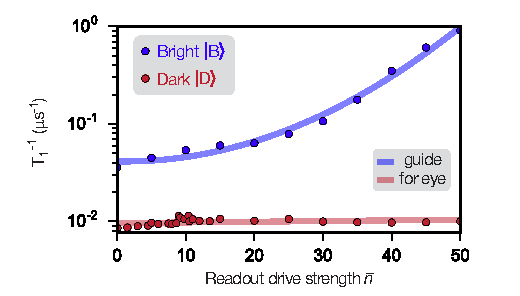
\includegraphics[scale=1.5]{results/T1-vs-nbar}
\par\end{centering}
\caption[Measurement-induced energy relaxation $T_{1}(\bar{n})$]{\label{fig:T1-vs-nbar}\textbf{Measurement-induced energy relaxation
$T_{1}(\bar{n})$.} Energy relaxation rate ($T_{1}^{-1}$) of $\ket{\mathrm{B}}$
(blue dots) and $\ket{\mathrm{D}}$ (red dots) as a function of $\bar{n}$,
measured with the following protocol: after the atom is prepared in
either $\ket{\mathrm{B}}$ or $\ket{\mathrm{D}}$, the readout tone
($\mathrm{R}$) is turned on for duration $t_{\mathrm{read}}$ with
amplitude $\bar{n}$ (corresponding to the number of steady-state
photons in the readout cavity when excited on resonance), whereafter,
the population of the initial state is measured. As in all other experiments,
the readout drive is applied at the $\ket{\mathrm{B}}$ cavity frequency
($\omega_{\mathrm{C}}-\chi_{\mathrm{B}}$). The relaxation rates are
extracted from exponential fits of the population decay as a function
of $t_{\mathrm{read}}$, from $1.3\times10^{7}$ experimental realizations.
The solids lines are guides to the eye: blue line indicates the rapid
degradation of $T_{1}^{\mathrm{B}}$ as a function of the readout
strength, while the red line indicates the nearly constants $T_{1}^{\mathrm{D}}$
of the protected dark level.}
\end{figure}


\section{Control of the three-level atom\label{sec:Control-of-the}}

\subsection{Qubit pulses\label{subsec:Qubit-pulses-calib}}

The implementation of precise and coherent manipulation of the three-level
atom is important for the tomographic reconstruction of the flight
of the quantum jump as well the ability to faithfully reverse it.
One of the main sources of pulse infidelity is typically decoherence,
but the rather long coherence time of the Darkmon device relative
to the duration of the pulses employed in the experiment make it largely
unimportant, and instead, place emphasis on the technical details
of pulse generation and Hamiltonian non-idealities, such as leakage
to higher excited states. 

Mitigation of main technical non-idealities. The effect of the zero-order
hold of the FPGA digital-to-analog converter (DAC) was mitigated by
installing a 270~MHz low pass filter (\textit{Mini-Circuits BLP-300+})
on each of the analog output channels, see Sec.~\ref{sec:Microwave-setup}.
All microwave tones were generated with single-sideband IQ-controlled
modulation at a base intermediate frequency (IF) of 50~MHz, and the
lower radio-frequency (RF) sideband was used for the control tones
(detuned 50~MHz below the local oscillator (LO) frequency). The IQ
mixers were calibrated with a four stage iterative routine to minimize
carrier leakage, by tuning the DC offsets of the I and Q channels,
and to suppress the RF image, by minimizing the quadrature skew and
IQ gain imbalance. The LO leakage could typically be suppressed to
$\approx-70$~dB relative to the RF tone. Spurious intermodulation
tones generated by higher-order non-linear terms present in the mixers
{[}i.e., third-order intercept-point (IP3) products{]} were generally
negligible as the mixers were not typically driven near saturation,
but bandpass filters were installed on the RF outputs of all mixers
to nonetheless suppress any spurious tones. Excess noise from the
following RF amplifier (\textit{MiniCircuits ZVA-183-S+}) was suppressed
by 80\,dB when the control drives were turned off by use of a high-isolation
SPST switch (\textit{Analog Device HMC-C019}).

The pulses applied to the Dark and Bright transition were calibrated
with a combination of Rabi, derivative removal via adiabatic gate
(DRAG) \citep{JChow2010-DRAG}, \emph{All-XY} \citep{Reed2013}, and
amplitude pulse train sequences \citep{Bylander2011}. Pulse timings
and delays, especially between the analog channels and the SPST switch
digital markers, were calibrated with a wide-bandwidth oscilloscope
with ultra-low jitter (\emph{Keysight 86100D Infiniium DCA-X}). The
alignment was verified by performing a Gaussian qubit $\pi$ pulse
on the GB transition and varying the delay between the rise of the
SPST digital marker and the signal on the analog IQ pair playing the
pulse. 


\subsection{Tomography of the three-level atom\label{subsec:Tomography-of-three-level}}

At the end of each experimental realization, we performed one of 15
rotation sequences on the atom that transferred information about
one component of the density matrix, $\hat{\rho}_{a}$, to the population
of $\ket{\mathrm{B}}$, which was measured with a 600~ns square pulse
on the readout cavity. Pulses were calibrated as discussed in Sec.~\ref{subsec:Qubit-pulses-calib}.
The readout signal was demodulated with the appropriate digital filter
function required to realize temporal mode matching \citep{Eichler2012-itinerant-entanglement}.
To remove the effect of potential systematic offset errors in the
readout signal, we subtracted the measurement results of operator
components of $\hat{\rho}_{a}$ and their opposites. From the measurement
results of this protocol, we reconstructed the density matrix $\hat{\rho}_{a}$,
and subsequently parametrized it the useful form 
\begin{equation}
\hat{\rho}_{a}=\begin{pmatrix}\frac{N}{2}\left(1-Z_{\mathrm{GD}}\right) & \frac{N}{2}\left(X_{\mathrm{GD}}+iY_{\mathrm{GD}}\right) & R_{\mathrm{BG}}+iI_{\mathrm{BG}}\\
\frac{N}{2}\left(X_{\mathrm{GD}}-iY_{\mathrm{GD}}\right) & \frac{N}{2}\left(1+Z_{\mathrm{GD}}\right) & R_{\mathrm{BD}}+iI_{\mathrm{BD}}\\
R_{\mathrm{BG}}-iI_{\mathrm{BG}} & R_{\mathrm{BD}}-iI_{\mathrm{BD}} & 1-N
\end{pmatrix},\label{eq:rhoa}
\end{equation}
where $X_{\mathrm{GD}},Y_{\mathrm{GD}},$ and $Z_{\mathrm{GD}}$ are
the Bloch vector components of the GD manifold, $N$ is the total
population of the $\ket{\mathrm{G}}$ and $\ket{\mathrm{D}}$ states,
while $R_{\mathrm{BG}},R_{\mathrm{BD}},I_{\mathrm{BG}}$ and $I_{\mathrm{BD}}$
are the coherences associated with $\ket{\mathrm{B}}$, relative to
the GD manifold. The measured population in $\ket{\mathrm{B}}$, $1-N$,
remains below 0.03 during the quantum jump, see Fig.~\ref{fig:tomo_tmid}.
Tomographic reconstruction was calibrated and verified by preparing
Clifford states, accounting for the readout fidelity of 97\%.

\paragraph{Control experiment.}

In Fig.~\ref{fig:time-resolved-tomo-D}, we show the results of a
control experiment where we verified the Ramsey coherence ($T_{\mathrm{2R}}^{\mathrm{D}}$)
and energy relaxation ($T_{\mathrm{1}}^{\mathrm{D}}$) times of the
DG transition with our tomography method. Solid lines are fitted theoretical
curves for the free evolution of the prepared initial state $\frac{1}{\sqrt{2}}\left(\D-\G\right)$.
The $T_{\mathrm{2R}}^{\mathrm{D}}=119.2\,\mathrm{\mu s}$ value gained
from the simultaneous fit of $X_{\mathrm{DG}}(t)$ and $Y_{\mathrm{DG}}(t)$
matches the lifetime independently obtained from a standard $T_{\mathrm{2R}}$
measurement. Similarly, the value of $T_{\mathrm{1}}^{\mathrm{D}}=115.4\,\mathrm{\mu s}$
extracted from an exponential fit of $Z_{\mathrm{DG}}(t)$ matches
the value obtained from a standard $T_{\mathrm{1}}$ measurement.
We note that our tomography procedure is well calibrated and skew-free,
as evident in the zero steady-state values of $X_{\mathrm{DG}}$ and
$Y_{\mathrm{DG}}$. The steady state $Z_{\mathrm{DG}}$ corresponds
to the thermal population of the dark state $n_{\mathrm{th}}^{\mathrm{D}}$.
It has recently been shown that residual thermal populations in cQED
systems can be significantly reduced by properly thermalizing the
input-output lines \citep{Yeh2017Atten,Wang2019-cav-atten}.

\begin{figure}
\begin{centering}
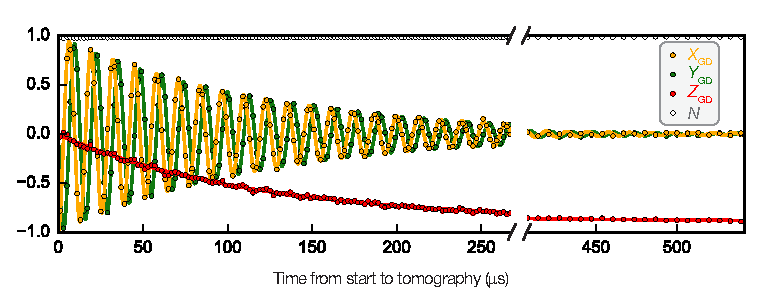
\includegraphics[scale=1.2]{results/time-resolved-tomo-D}
\par\end{centering}
\caption[Control experiment: time-resolved tomogram of the free evolution of
a DG superposition]{\label{fig:time-resolved-tomo-D}\textbf{Control experiment: time-resolved
tomogram of the free evolution of a DG superposition. }The atom is
prepared in $\frac{1}{\sqrt{2}}\left(\D-\G\right)$ and tomography
is performed after a varied delay. Dots: reconstructed conditional
GD tomogram ($X_{\mathrm{DG}},Y_{\mathrm{DG}}$, and $Z_{\mathrm{DG}}$)
and population in DG manifold, $N$, see Eq.~(\ref{eq:rhoa}). Solid
lines: theoretical fits. }
\end{figure}


\paragraph{Mid-flight tomogram.}

In the presence of the coherent Rabi drive $\Odg$ (corresponding
to catch parameter $\Delta t_{\mathrm{off}}=0$), the complete tomogram
of the three-level atom was reconstructed, and a slice at the mid-flight
time, $\Delta t_{\mathrm{mid}}$, is shown in Fig.~\ref{fig:tomo_tmid}.
All imaginary components of the reconstructed conditional density
matrix, $\rho_{\mathrm{c}}$, are negligibly small, less than 0.007,
as expected, see Sec.~\ref{subsec:Comparison-between-theory}, for
well-calibrated tomographic phase control. The population of the $\B$
state, 0.023, is nearly negligible as well, as it is conditioned away
by the IQ filter, see Sec.~\ref{subsec:IQ-filter}.
\begin{figure}
\centering{}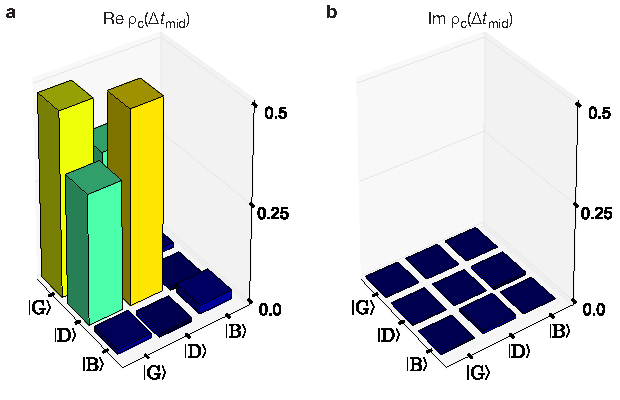
\includegraphics[width=120mm]{results/tomogram_tmid}
\caption[Mid-flight tomogram]{\label{fig:tomo_tmid}\textbf{Mid-flight tomogram. }The plots show
the real (a) and imaginary (b) parts of the conditional density matrix,
$\rho_{\mathrm{c}}$, at the mid flight of the quantum jump ($\Delta t_{\mathrm{catch}}=\Delta t_{\mathrm{mid}}$),
in the presence of the Rabi drive from $\ket{\mathrm{G}}$ to $\ket{\mathrm{D}}$
($\Delta t_{\mathrm{off}}=0$). The population of the $\ket{\mathrm{B}}$
state is 0.023, and the magnitude of all imaginary components is less
than 0.007. }
\end{figure}


\subsection{Atom and cavity drives \label{subsec:Atom-and-cavity}}

In all experiments, unless noted otherwise, the following drive parameters
were used: The DG Rabi drive, $\Omega_{\mathrm{DG}}$, was applied
275~kHz below $\omega_{\mathrm{D}}$ to account for the Stark shift
of the cavity. The BG drive, $\Omega_{\mathrm{BG}}$, was realized
as a bi-chromatic tone in order to unselectively address the BG transition,
which was broadened and Stark shifted due to the coupling between
$\ket{\mathrm{B}}$ and the readout cavity. Specifically, we addressed
transitions from $\ket{\mathrm{G}}$ to $\ket{\mathrm{B}}$ with a
Rabi drive $\Omega_{\mathrm{B0}}/2\pi=1.20\pm0.01\,$~MHz at frequency
$\omega_{\mathrm{BG}}$, whereas transitions from $\ket{\mathrm{B}}$
to $\ket{\mathrm{G}}$ were addressed with a Rabi drive $\Omega_{\mathrm{B1}}/2\pi=0.60\pm0.01\,$~MHz
tuned 30~MHz below $\omega_{\mathrm{BG}}$. This bi-chromatic scheme
provided the ability to tune the up-click and down-click rates independently,
but otherwise essentially functioned as an incoherent broad-band source.
In Table~\ref{tab:Summary-of-timescales.}, we summarize the hierarchy
of timescales established by the drive amplitudes and frequencies
as well as the relevant decoherence properties of the atom.

\begin{table}[!ht]
\begin{centering}
\addtolength{\tabcolsep}{2pt} 
\renewcommand*{\arraystretch}{1.5}
 %
\begin{tabular}{cc>{\raggedright}p{0.65\columnwidth}}
\hline 
\textbf{Symbol}  & \textbf{Value}  & \textbf{Description}\tabularnewline
\hline 
$\Gamma^{-1}$  & $\approx8.8$\,ns  & Effective measurement time of $\ket{\mathrm{B}}$, approximately given
by $1/\kappa\bar{n}$, where $\bar{n}=5\pm0.2$ in the main experiment\tabularnewline
$\kappa^{-1}$  & $44.0\pm0.06$\,ns  & Readout cavity lifetime\tabularnewline
$T_{\mathrm{int}}$  & 260.0\,ns  & Integration time of the measurement record, set in the controller
at the beginning of the experiment \tabularnewline
$\Gamma_{\mathrm{BG}}^{-1}$  & $0.99\pm0.06\,\mathrm{\mu s}$  & Average time the atom rests in $\ket{\mathrm{G}}$ before an excitation
to $\ket{\mathrm{B}}$, see Fig.~\ref{fig:jumps}b\tabularnewline
$\Delta t_{\mathrm{mid}}$  & $3.95\,\mathrm{\mu s}$  & No-click duration for reaching $Z_{\mathrm{GD}}=0$ in the flight
of the quantum jump from $\ket{\mathrm{G}}$ to $\ket{\mathrm{D}}$,
in the full presence of $\Omega_{\mathrm{DG}}$, see Fig.~\ref{fig:catch}b\tabularnewline
$\Gamma_{\mathrm{GD}}^{-1}$  & $30.8\pm0.4\,\mathrm{\mu s}$  & Average time the atom stays in $\ket{\mathrm{D}}$ before returning
to $\ket{\mathrm{G}}$ and being detected, see Fig.~\ref{fig:jumps}b\tabularnewline
$T_{1}^{\mathrm{D}}$  & $116\pm5\,\mathrm{\mu s}$  & Energy relaxation time of $\ket{\mathrm{D}}$\tabularnewline
$T_{2\mathrm{R}}^{\mathrm{D}}$  & $120\pm5\,\mathrm{\mu s}$  & Ramsey coherence time of $\ket{\mathrm{D}}$\tabularnewline
$T_{2\mathrm{E}}^{\mathrm{D}}$  & $162\pm6\,\mathrm{\mu s}$  & Echo coherence time of $\ket{\mathrm{D}}$\tabularnewline
$\Gamma_{\mathrm{DG}}^{-1}$  & $220\pm5\,\mathrm{\mu s}$  & Average time between two consecutive $\ket{\mathrm{G}}$ to $\ket{\mathrm{D}}$
jumps\tabularnewline
\end{tabular}
\par\end{centering}
\caption[Summary of timescales]{\textbf{Summary of timescales. }List of the characteristic timescales
involved in the catch and reverse experiment. The Hamiltonian parameters
of the system are summarized in Sec.~\ref{sec:Characterization-of-the}.
\textbf{\label{tab:Summary-of-timescales.}}}
\end{table}


\section{Monitoring quantum jumps in real time }

\subsection{IQ filter \label{subsec:IQ-filter}}

To mitigate the effects of imperfections in the atom readout scheme
in extracting a $\ket{\mathrm{B}}$/not-$\ket{\mathrm{B}}$ result,
we applied a two-point, hysteretic IQ filter, implemented on the FPGA
controller in real time. The filter is realized by comparing the present
quadrature record values $\left\{ I_{\mathrm{rec}},Q_{\mathrm{rec}}\right\} $,
with three thresholds ($I_{\mathrm{B}},I_{\bar{\mathrm{B}}},$ and
$Q_{\mathrm{B}}$) in the following way: 
\begin{center}
\begin{tabular}{>{\raggedleft}m{20mm}|>{\centering}p{30mm}|>{\centering}p{30mm}|>{\centering}p{30mm}}
\textbf{Input: } & $Q_{\mathrm{rec}}\geq Q_{\mathrm{B}}$ or

$I_{\mathrm{rec}}>I_{\mathrm{B}}$  & $Q_{\mathrm{rec}}<Q_{\mathrm{B}}$ and

$I_{\mathrm{rec}}<I_{\bar{\mathrm{B}}}$  & $Q_{\mathrm{rec}}<Q_{\mathrm{B}}$ and

$I_{\bar{\mathrm{B}}}\leq I_{\mathrm{rec}}\leq I_{\mathrm{B}}$\tabularnewline
\hline 
\textbf{Output: } & $\ket{\mathrm{B}}$  & not-$\ket{\mathrm{B}}$  & previous\tabularnewline
\end{tabular}
\par\end{center}

\noindent The filter and thresholds were selected to provide a best
estimate of the time of a click, operationally understood as a change
in the filter output from $\ket{\mathrm{B}}$ to not-$\ket{\mathrm{B}}$.
The $I_{{\mathrm{B}}}$ and $I_{\bar{\mathrm{B}}}$ thresholds were
chosen 1.5 standard deviations away from the I-quadrature mean of
the $\ket{\mathrm{B}}$ and not-$\ket{\mathrm{B}}$ distributions,
respectively. The $Q_{{\mathrm{B}}}$ threshold was chosen 3 standard
deviations away from the Q-quadrature mean. Higher excited states
of the atom were selected out by $Q_{\mathrm{rec}}$ values exceeding
the $Q_{\mathrm{B}}$ threshold. 

\subsection{Unconditioned monitoring}

In Sec.~\ref{sec:Unconditioned-monitoring-of}, we described a protocol
for the unconditioned monitoring of the quantum jumps where the atom
is subject to the continuous Rabi drives $\Omega_{\mathrm{BG}}$ and
$\Omega_{\mathrm{DG}}$, as depicted in Fig.~\ref{fig:setup}. From
the continuous tracking of the quantum jumps, over 3.2~s. of data,
we histogrammed the times, $\tau_{\operatorname{not-B}}$, spent in
not-$\ket{\mathrm{B}}$, Fig.~\ref{fig:jumps}b. In Fig.~\ref{fig:B-wait-time},
we show the complimentary histogram for the times, $\tau_{{\rm B}},$
spent in $\B$, which is unlike the latter, in that it follows a single
exponential decay law. This single Poisson process character follows
from the fact that the $\B$ measurement result collapses the atom
to a single state, $\B$, unlike the not-$\B$ result. The average
time spent in $\B$, extracted from the fit, is $\bar{\tau}_{{\rm B}}=4.2\pm0.03\,\mathrm{\mu s}$.
\begin{figure}
\centering{}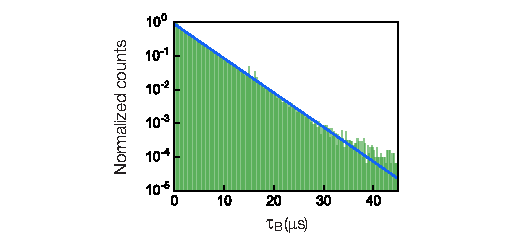
\includegraphics[width=145mm]{results/B_waiting_time}
\caption[Waiting time to switch from a $\B$ to not-$\B$ state assignment
result]{\label{fig:B-wait-time}\textbf{Waiting time to switch from a $\B$
to not-$\B$ state assignment result.} Semi-log plot of the histogram
(shaded green) of the duration of times corresponding to $\B$-measurement
results, $\tau_{\operatorname{B}}$, for 3.2~s of continuous data
of the type shown in Fig.~\ref{fig:jumps}a. Solid line is an exponential
fit, which yields a $4.2\pm0.03\,\mathrm{\mu s}$ time constant. }
\end{figure}

\pagebreak{}

\section{Catching and reversing the jump \label{sec:Catching-and-reversing}}

\subsection{Experiment flow}

\begin{figure}
\begin{centering}
%\hspace*{-1cm} % manually align to center of page 
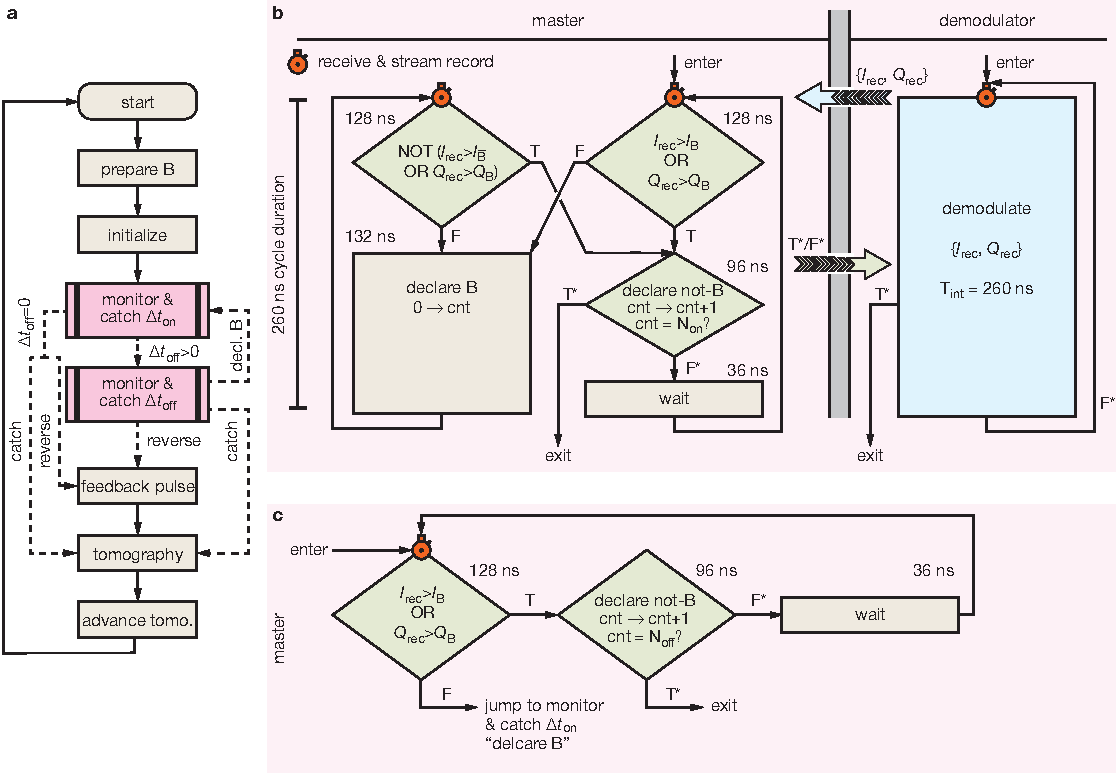
\includegraphics[angle=-90,scale=1.1]{results/experiment_flow}
\par\end{centering}
\caption[Experiment flow]{\label{fig:experiment-flow}\textbf{Experiment flow. }See text for
detailed description.}
\end{figure}
Figure \ref{fig:experiment-flow}a shows a flowchart representation
of steps involved in the catch and reverse protocol. In the following,
we describe each block in the diagram in the order in which it would
be executed.

\paragraph{Start:}

internal memory registers are set to zero \citep{Ofek2016,Liu2016Thesis},
including the no-click counter ``cnt,'' defined below. 

\paragraph{Prepare B:}

controller deterministically prepares the atom in $\ket{\mathrm{B}}$,
a maximally conservative initial state, with measurement-based feedback
\citep{Riste2012-qubit-measure-reset}. 

\paragraph{Initialize:}

controller turns on the atom ($\Omega_{\mathrm{BG}}$ and $\Omega_{\mathrm{DG}}$)
and cavity drives ($\mathrm{R}$) and begins demodulation. 

\paragraph{Monitor and catch $\Delta t_{\mathrm{on}}$: }

with all drives on ($\Omega_{\mathrm{BG}},\Omega_{\mathrm{DG}}$,
and $\mathrm{R}$), the controller actively monitors the cavity output
signal until it detects no-clicks for duration $\Delta t_{\mathrm{on}}$,
as described in panel (b), whereafter, the controller proceeds to
``monitor and catch $\Delta t_{\mathrm{off}}$'' in the case that
$\Delta t_{\mathrm{off}}>0$; otherwise, for $\Delta t_{\mathrm{off}}=0$,
the controller proceeds to ``tomography'' (``feedback pulse'')
for the catch (reverse) protocol.

\paragraph{Monitor and catch $\Delta t_{\mathrm{off}}$: }

with the Rabi drive $\Omega_{\mathrm{DG}}$ off, while keeping the
drives $\Omega_{\mathrm{BG}}$ and R on, the controller continues
to monitor the output signal. The controller exits the routine only
if it detects a click, proceeding to the ``declare B'' step of the
``monitor and catch $\Delta t_{\mathrm{on}}$'' routine, or if no
further clicks are detected for the pre-defined duration $\Delta t_{\mathrm{off}}$,
proceeding to ``tomography'' (``feedback pulse'') for the catch
(reverse) protocol.

\paragraph{Feedback pulse: }

with all the continuous drives turned off, the controller performs
a pulse on the DG transition of the atom, defined by the two angles
$\left\{ \theta_{I}\left(\Delta t_{\mathrm{catch}}\right),\varphi_{I}\left(\Delta t_{\mathrm{catch}}\right)\right\} $.

\paragraph{Tomography: }

controller performs next-in-order tomography sequence (see Sec.~\ref{subsec:Tomography-of-three-level})
while the demodulator finishes processing the final data in its pipeline.

\paragraph{Advance tomo.: }

tomography sequence counter is incremented, and after a $50~\mathrm{\mu s}$
delay, the next realization of the experiment is started.

\subsubsection{Logic and timing of catch subroutines}

\paragraph{Monitor and catch $\Delta t_{\mathrm{on}}$.}

Figure \ref{fig:experiment-flow}b shows a concurrent-programming
flowchart representation of the ``monitor and catch $\Delta t_{\mathrm{on}}$''
routine. Displayed are the master and demodulator modules of the controller.
The demodulator outputs a pair of 16 bit signed integers, $\left\{ I_{\mathrm{rec}},Q_{\mathrm{rec}}\right\} $,
every $T_{\mathrm{int}}=260$~ns, which is routed to the master module,
as depicted by the large left-pointing arrow. The master module implements
the IQ filter (see Sec.~\ref{subsec:IQ-filter}) and tracks the number
of consecutive not-$\ket{\mathrm{B}}$ measurement results with the
counter cnt. The counter thus keeps track of the no-click time elapsed
since the last click, which is understood as a change in the measurement
result from $\ket{\mathrm{B}}$ to not-$\ket{\mathrm{B}}$. When the
counter reaches the critical value $N_{\mathrm{on}}$, corresponding
to $\Delta t_{\mathrm{on}}$, the master and demodulator modules synchronously
exit the current routine, see the T{*} branch of the ``declare not-B''
decision block. Until this condition is fulfilled (F{*}), the two
modules proceed within the current routine as depicted by the black
flowlines. 

To minimize latency and maximize computation throughput, the master
and demodulator were designed to be independent sequential processes
running concurrently on the FPGA controller, communicating strictly
through synchronous message passing, which imposed stringent synchronization
and execution time constraints. All master inter-module logic was
constrained to run at a 260~ns cycle, the start of which necessarily
was imposed to coincide with a ``receive \& stream record'' operation,
here, denoted by the stopwatch. In other words, this imposed the algorithmic
constraint that all flowchart paths staring at a stopwatch and ending
in a stopwatch, itself or other, were constrained to a 260\,ns execution
timing. A second key timing constraint was imposed by the time required
to propagate signals between the different FPGA cards, which corresponded
to a minimum branching-instruction duration of 76~ns.

\paragraph{Monitor and catch $\Delta t_{\mathrm{off}}$.}

Figure \ref{fig:experiment-flow}c shows a concurrent-programming
flowchart representation of the master module of the ``monitor and
catch $\Delta t_{\mathrm{off}}$'' routine. The corresponding demodulation-module
flowchart is identical to that shown of panel (b); hence, it is not
shown. This routine functions in following manner: If a $\ket{\mathrm{B}}$
outcome is detected, the controller jumps to the ``declare B'' block
of the monitor \& catch $\Delta t_{\mathrm{on}}$ routine; otherwise,
when only not-$\ket{\mathrm{B}}$ outcomes are observed, and the counter
reaches the critical value $N_{\mathrm{off}}$, corresponding to $\Delta t_{\mathrm{catch}}=\Delta t_{\mathrm{on}}+\Delta t_{\mathrm{off}}$,
the controller exits the routine.

\section{Comparison between theory and experiment \label{subsec:Comparison-between-theory}\label{subsec:Error-analysis}}

In this section, we present the comparison between the results of
the quantum jumps experiment and the predictions of the quantum trajectory
theory of the experiment developed in Chapter~\ref{chap:theoretical-description-jumps}.
The results agree with the theoretical predictions, accounting for
known imperfections, essentially without adjustable parameters. Simulation
plots courtesy of H.J. Carmichael. 

\subsection{Simulated data sets}

\paragraph{\textit{\emph{Independently measured parameters.}}}

The parameters used in the Monte Carlo simulation described in Sec.~\ref{subsec:Simulation-of-linear}
are listed in Table~\ref{table:table2}. Nearly all are set to the
value at the center of the range quoted in Table~\ref{tab:system-params},
with three exceptions: i) $T_{1}^{{\rm B}}$ and $T_{1}^{{\rm D}}$
are set to lower values in response to the photon number dependence
of the readout displayed in Fig.~\ref{fig:T1-vs-nbar}, ii) $\Omega_{{\rm DG}}/2\pi$
is set higher, but still falls inside the experimental error bars,
and iii) $n_{{\rm th}}^{{\rm C}}=0$. Notably, of the three exceptions,
only $\Omega_{{\rm DG}}/2\pi$ has a noticeable effect on the comparison
between simulated and experimental data sets.

\paragraph{\textit{\emph{Leakage from the }}\emph{GBD}\textit{\emph{-manifold.}}\emph{ }}

As discussed in Sec.~\ref{sec:circuit-design}, see Fig.~\ref{fig:Darkmon-energy-level-diagram},
the Darkmon system has higher excited states, which are generally
unimportant, but do contribute a small imperfection that needs to
be considered to qualitatively account for the results. As discussed
in Sec.~\ref{subsec:Simulation-of-linear}, we model the effect of
leakage from the GBD manifold by adding a single additional higher-excited
state level, denoted $\ket{\mathrm{F}}.$ The additional random jumps
to state $|{\rm F}\rangle$ are governed by four parameters that are
not independently measured; they serve as fitting parameters, required
to bring the simulation into agreement with the asymptotic behavior
of ${\rm Z}(\Delta t_{{\rm catch}})$, which, without leakage to $|{\rm F}\rangle$,
settles to a value higher than is measured in the experiment. The
evolution of the ${\rm X}(\Delta t_{{\rm catch}})$ is largely unaffected
by the assignment of these parameters, where any change that does
occur can be offset by adjusting $\Omega_{{\rm DG}}/2\pi$ while staying
within the experimental error bars.

\paragraph{\textit{\emph{Ensemble average.}}\emph{ }}

Simulated data sets are computed as an ensemble average by sampling
an ongoing Monte Carlo simulation, numerically implementing the model
outlined in Eqs.~(\ref{eqn:SSE_continuous})--(\ref{eqn:jumps_to_F}).
Quadratures $I_{{\rm rec}}$ and $Q_{{\rm rec}}$ are computed from
Eqs.~(\ref{eqn:simulated_I_int}) and (\ref{eqn:simulated_Q_int}),
digitized with integration time $T_{{\rm int}}=260\mkern2mu {\rm ns}$,
and then, as in the experiment, a hysteric filter is used to locate
``click'' events ($\Delta t_{{\rm catch}}=0$) corresponding to
an inferred change of state from $|{\rm B}\rangle$ to not-$|{\rm B}\rangle$.
During the subsequent sampling interval ($\Delta t_{{\rm catch}}\geq0$),
the four quantities 
\begin{equation}
\big({\rm Z}_{{\rm GD}}^{j},{\rm X}_{{\rm GD}}^{j},{\rm Y}_{{\rm GD}}^{j},{\rm P}_{{\rm BB}}^{j}\big)(\Delta t_{{\rm catch}})=\big({\rm Z}_{{\rm GD}}^{{\rm rec}},{\rm X}_{{\rm GD}}^{{\rm rec}},{\rm Y}_{{\rm GD}}^{{\rm rec}},{\rm P}_{{\rm BB}}^{{\rm rec}}\big)(t_{j}+\Delta t_{{\rm catch}}),
\end{equation}
with $t_{j}$ is the click time and 
\begin{eqnarray}
{\rm Z}_{{\rm GD}}^{{\rm rec}}(t) & = & \frac{\langle{\rm D}|\psi(t)\rangle\langle\psi(t)|{\rm D}\rangle-\langle{\rm G}|\psi(t)\rangle\langle\psi(t)|{\rm G}\rangle}{\langle\psi(t)|\psi(t)\rangle},\label{eqn:correlated_Z_GD}\\
\noalign{\vskip4pt}{\rm X}_{{\rm GD}}^{{\rm rec}}(t)+i{\rm Y}_{{\rm GD}}^{{\rm rec}}(t) & = & 2\frac{\langle{\rm D}|\psi(t)\rangle\langle\psi(t)|{\rm G}\rangle}{\langle\psi(t)|\psi(t)\rangle},\label{eqn:correlated_X_GD=000026Y_GD}\\
\noalign{\vskip4pt}{\rm P}_{{\rm BB}}^{{\rm rec}}(t) & = & \frac{\langle{\rm B}|\psi(t)\rangle\langle\psi(t)|{\rm B}\rangle}{\langle\psi(t)|\psi(t)\rangle},
\end{eqnarray}
are computed, and running sums of each are updated. The sample terminates
when the measurement record indicates a change of state from not-$|{\rm B}\rangle$
back to $|{\rm B}\rangle$. Finally, for comparison with the experiment,
Bloch vector components are recovered from the average over sample
intervals via the formula 
\begin{equation}
\big({\rm Z}_{{\rm GD}},{\rm X}_{{\rm GD}},{\rm Y}_{{\rm GD}}\big)(\Delta t_{{\rm catch}})=\frac{\sum_{j}^{N(\Delta t_{{\rm catch}})}\big({\rm Z}_{{\rm GD}}^{j},{\rm X}_{{\rm GD}}^{j},{\rm Y}_{{\rm GD}}^{j}\big)(\Delta t_{{\rm catch}})}{N(\Delta t_{{\rm catch}})-\sum_{j}^{N(\Delta t_{{\rm catch}})}P_{{\rm BB}}^{j}(\Delta t_{{\rm catch}})},\label{eqn:ensemble_average}
\end{equation}
where $N(\Delta t_{{\rm catch}})$ is the number of sample intervals
that extend up to, or beyond, the time $\Delta t_{{\rm catch}}$.
The simulation and sampling procedure is illustrated in Fig.~\ref{fig:monte-carlo},
and a comparison between the experiment and the simulation is provided
in Fig.~\ref{fig:simulation_vs_experiment}.

The simulated and measured Bloch vector components are fit with expressions
motivated by Eqs.~(\ref{eqn:Z_approx})-(\ref{eqn:Y_approx}) and~(\ref{eq:ZGDXGD-long-term}),
modified to account for the effect of non-idealities in the experiment,
\begin{align}
\mathrm{Z}_{\text{GD}}(\Delta t_{\operatorname{catch}}) & =\ensuremath{a+b\tanh(\Delta t_{\operatorname{catch}}/\tau+c)},\\
\ensuremath{\mathrm{X}_{\text{GD}}(\Delta t_{\operatorname{catch}})} & =a'+b'\operatorname{sech}(\Delta t_{\operatorname{catch}}/\tau'+c')\,,\\
\mathrm{Y}_{\text{GD}}(\Delta t_{\operatorname{catch}}) & =0\,.
\end{align}
The fit parameters ($a,a',b,b',c,c',\tau,\tau'$) for the simulated
and experimental data shown in Fig.~\ref{fig:simulation_vs_experiment}
are compared in Table~\ref{tab:Comparison-of-parameters}. As imposed
by Eq.~(\ref{eq:ZGDXGD-long-term}), in the absence of $\Omega_{{\rm DG}}$
(turned off at time $\Delta t_{{\rm on}}=2\mkern2mu \mu{\rm s}$)
$a'$, the offset of $\mathrm{X}_{\text{GD}}$, is strictly enforced
to be zero. The extracted simulation and experiment parameters are
found to agree at the percent level.

\begin{table}[t]
\begin{centering}
\renewcommand*\arraystretch{1.5}
%\hspace*{-1.2cm} % manually align to center of page 
\begin{tabular}{rl|rl|rl}
\multicolumn{2}{c|}{\textbf{Readout cavity}} & \multicolumn{2}{c|}{\textbf{BG transition}} & \multicolumn{2}{c}{\textbf{DG transition}}\tabularnewline
\hline 
\hline 
\multicolumn{6}{c}{\textbf{\rule{0pt}{5ex}Non-linear parameters}}\tabularnewline
\hline 
 &  & $\chi_{\mathrm{B}}/2\pi=$ & $-5.08\,\mathrm{MHz}$~ & $\chi_{\mathrm{D}}/2\pi=$ & $-0.33\,\mathrm{MHz}$\tabularnewline
\multicolumn{6}{c}{\textbf{\rule{0pt}{5ex}Coherence related parameters}}\tabularnewline
\hline 
\textbf{\rule{0pt}{5ex}}$\kappa/2\pi$= & $3.62\mathrm{MHz}$ & $T_{\mathrm{1}}^{\mathrm{B}}=$ & $15\,\mathrm{\mu s}$ & $T_{\mathrm{1}}^{\mathrm{D}}=$ & $105\,\mathrm{\mu s}$\tabularnewline
$\eta=$ & $0.33$ & $T_{\mathrm{2\mathrm{R}}}^{\mathrm{B}}=$ & $18\,\mathrm{\mu s}$ & $T_{\mathrm{2\mathrm{R}}}^{\mathrm{D}}=$ & $120\,\mathrm{\mu s}$\tabularnewline
$T_{\mathrm{int}}=$ & $260.0\,\mathrm{ns}$ &  &  &  & \tabularnewline
$n_{\mathrm{th}}^{\mathrm{C}}=$ & $0$ & $n_{\mathrm{th}}^{\mathrm{B}}=$ & $0.01$ & $n_{\mathrm{th}}^{\mathrm{D}}=$ & $0.05$\tabularnewline
\multicolumn{6}{c}{\textbf{\rule{0pt}{5ex}Drive amplitude and detuning parameters}}\tabularnewline
\hline 
\textbf{\rule{0pt}{5ex}}$\bar{n}=$ & $5.0$ & ~$\Omega_{\mathrm{B}0}/2\pi=$ & $1.20\,\mathrm{MHz}$ & ~$\Omega_{\mathrm{DG}}/2\pi=$ & $21.6\,\mathrm{kHz}$\tabularnewline
 &  & ~$\Omega_{\mathrm{B}1}/2\pi=$ & $0.60\,\mathrm{MHz}$ &  & \tabularnewline
$\Delta_{\mathrm{R}}=$ & $\chi_{\mathrm{B}}$ & ~$\Delta_{\mathrm{B}1}/2\pi=$ & $-30.0\,\text{MHz}$ & ~$\Delta_{\mathrm{DG}}/2\pi=$ & $-274.5\,\text{kHz}$\tabularnewline
\end{tabular}
\par\end{centering}
\caption[Compilation of the simulation parameters]{\textbf{Compilation of the simulation parameters.}}
\label{table:table2} 
\end{table}

\begin{figure}[t]
\centering{}\includegraphics[width=145mm]{results/SamplingMC}\caption[Sampling of the Monte-Carlo simulation (courtesy of H.J. Carmichael)]{\label{fig:monte-carlo} \textbf{Sampling of the Monte-Carlo simulation.}
\textbf{a,} Simulated measurement quadrature $I_{{\rm rec}}$ and
correlated trajectory computed from Eqs.~(\ref{eqn:correlated_Z_GD})
and (\ref{eqn:correlated_X_GD=000026Y_GD}). Three sample intervals
are shown. The earliest corresponds to leakage from the GBD-manifold,
where a jump from $|{\rm G}\rangle$ to $|{\rm F}\rangle$ is followed
by a jump from $|{\rm F}\rangle$ to $|{\rm D}\rangle$. The second
and third sample intervals correspond to direct transitions from $|{\rm G}\rangle$
to $|{\rm D}\rangle$, which are continuously monitored and the object
of the experiment. \textbf{b,} Expanded view of the shaded region
of the second sample interval in panel (a). The evolution is continuous
but not smooth, due to backaction noise from the continuously monitored
readout. This feature is in sharp contrast to the perfect ``no-click''
readout upon which the simple theory of Sec.~\ref{sec:Fluorescence-monitored-by}
is based. Figure courtesy of H.J. Carmichael.}
\end{figure}

\begin{figure}
\centering{}\includegraphics[width=120mm]{results/tomoCompar}\caption[Comparison between simulation and experiment (courtesy of H.J. Carmichael)]{\label{fig:simulation_vs_experiment} \textbf{Comparison between
simulation and experiment.} \textbf{a,} Simulated data set obtained
with Rabi drive $\Omega_{{\rm DG}}$ turned on for the entire $\Delta t_{{\rm catch}}$;
parameters taken from Table \ref{table:table2} and leakage from the
GBD-manifold included with $(\gamma_{{\rm FG}},\gamma_{{\rm FD}})/2\pi=0.38\mkern2mu {\rm kHz}$
and $(\gamma_{{\rm GF}},\gamma_{{\rm DF}})/2\pi=11.24\mkern2mu {\rm kHz}$.
\textbf{b,} Simulated data set obtained with Rabi drive $\Omega_{{\rm DG}}$
turned off at time $\Delta t_{{\rm on}}=2\mkern2mu \mu{\rm s}$; parameters
taken from Table \ref{table:table2} and leakage from the GBD-manifold
included with $\gamma_{{\rm FG}}/2\pi=0.217\mkern2mu {\rm kHz}$,
$\gamma_{{\rm FD}}/2\pi=4.34\mkern2mu {\rm kHz}$, $\gamma_{{\rm GF}}/2\pi=11.08\mkern2mu {\rm kHz}$,
and $\gamma_{{\rm DF}}/2\pi=15.88\mkern2mu {\rm kHz}$. When leakage
from the GBD-manifold is omitted, the ${\rm Z}_{{\rm GD}}$ curve
rises more sharply and settles to a value that is 10\% (20\%) higher
in panel (a) (panel (b)). Figure courtesy of H.J. Carmichael.}
\end{figure}

\clearpage{}

\begin{table}
\begin{centering}
\begin{tabular}{c}
\textbf{(a)} In presence of $\Omega_{\mathrm{DG}}$\tabularnewline
\tabularnewline
\centering{}\renewcommand*{\arraystretch}{1.2} %
\begin{tabular}{cc|crcllrrlcr}
Parameter  & \multicolumn{1}{c|}{} &  & \multicolumn{3}{c}{Experiment} &  & \multicolumn{3}{c}{Simulation} &  & Error\tabularnewline
\hline 
\rule{0pt}{3ex} $a$  &  &  & -0.07  & $\pm$  & 0.005  &  & -0.07  & $\pm$  & 0.005  &  & 0.5\%\tabularnewline
$a'$  &  &  & -0.21  & $\pm$  & 0.005  &  & -0.22  & $\pm$  & 0.005  &  & 2\%\tabularnewline
$b$  &  &  & 0.94  & $\pm$  & 0.005  &  & 0.95  & $\pm$  & 0.005  &  & 1\%\tabularnewline
$b'$  &  &  & 0.93  & $\pm$  & 0.005  &  & 0.91  & $\pm$  & 0.005  &  & 2\%\tabularnewline
$c$  &  &  & -2.32  & $\pm$  & 0.03  &  & -2.27  & $\pm$  & 0.03  &  & 2\%\tabularnewline
$c'$  &  &  & -2.04  & $\pm$  & 0.03  &  & -2.05  & $\pm$  & 0.03  &  & 0.5\%\tabularnewline
$\tau$  &  &  & 1.64  & $\pm$  & 0.01  &  & 1.65  & $\pm$  & 0.01  &  & 0.5\%\tabularnewline
$\tau'$  &  &  & 1.74  & $\pm$  & 0.01  &  & 1.76  & $\pm$  & 0.01  &  & 1\%\tabularnewline
\end{tabular}\tabularnewline
\tabularnewline
\textbf{(b)} In absence of $\Omega_{\mathrm{DG}}$\tabularnewline
\tabularnewline
\centering{}\renewcommand*{\arraystretch}{1.2} %
\begin{tabular}{cc|crcllrrlcr}
Parameter & \multicolumn{1}{c|}{} &  & \multicolumn{3}{c}{Experiment} &  & \multicolumn{3}{c}{Simulation} &  & Error\tabularnewline
\hline 
\rule{0pt}{3ex} $a$ &  &  & -0.11 & $\pm$ & 0.005 &  & -0.10 & $\pm$ & 0.005 &  & 8\%\tabularnewline
$a'$ &  &  & 0 & $\pm$ & 0 &  & 0 & $\pm$ & 0 &  & 0\%\tabularnewline
$b$ &  &  & 0.92 & $\pm$ & 0.008 &  & 0.91 & $\pm$ & 0.008 &  & 1\%\tabularnewline
$b'$ &  &  & 0.61 & $\pm$ & 0.005 &  & 0.60 & $\pm$ & 0.005 &  & 2\%\tabularnewline
$c$ &  &  & -1.96 & $\pm$ & 0.05 &  & -2.10 & $\pm$ & 0.05 &  & 7\%\tabularnewline
$c'$ &  &  & -1.97 & $\pm$ & 0.05 &  & -2.05 & $\pm$ & 0.05 &  & 4\%\tabularnewline
$\tau$ &  &  & 2.17 & $\pm$ & 0.05 &  & 2.03 & $\pm$ & 0.05 &  & 6\%\tabularnewline
$\tau'$ &  &  & 1.98 & $\pm$ & 0.05 &  & 1.92 & $\pm$ & 0.05 &  & 3\%\tabularnewline
\end{tabular}\tabularnewline
\tabularnewline
\end{tabular}
\par\end{centering}
\caption[Comparison between parameters extracted from the simulation and those
from the experiment. ]{\label{tab:Comparison-of-parameters} \textbf{Comparison between
parameters extracted from the simulation and those from the experiment}.
\textbf{a,} Parameters obtained from fits of the simulated and measured
data for the catch protocol in the presence of the Rabi drive $\Omega_{{\rm DG}}$
throughout the entire duration of the quantum jump, data shown in
Fig.~\ref{fig:simulation_vs_experiment}a. \textbf{b,} Parameters
obtained from fits of the simulated and measured data for the catch
protocol in the absence of the $\Omega_{{\rm DG}}$ during the flight
of the quantum jump for $\Delta t_{\mathrm{on}}=2\mathrm{\ \mu s}$,
data shown in Fig.~\ref{fig:simulation_vs_experiment}b. }
\end{table}

\clearpage{}

\subsection{Error budget\label{sec:Budget-coherence}}

In this section, we examine the effect of the various imperfections
and dissipation channels on the fidelity of the catch protocol. 

\paragraph{\textit{\emph{Imperfections.}}}

The various imperfections are expected to reduce the maximum coherence
recovered in the measurement of ${\rm X}_{{\rm GD}}(\Delta t_{{\rm catch}})$.
They include: 
\begin{enumerate}
\item Readout errors when inferring $|{\rm B}\rangle$ to not-$|{\rm B}\rangle$
transitions and the reverse. Such errors affect the assignment of
$\Delta t_{{\rm catch}}$, which can be either too short or too long
to correlate correctly with the true state of the system. 
\item Leaks from the GBD-manifold to higher excited states. Importantly,
these errors mimic a $|{\rm B}\rangle$ to not-$|{\rm B}\rangle$
transition, as in the first sample interval of Fig.~\ref{fig:monte-carlo},
but the anticipated coherent evolution within the GBD-manifold does
not occur. In this manner, the excitations to higher states lead to
false detections.
\item Thermal jumps from $|{\rm G}\rangle$ to $|{\rm D}\rangle$. Such
incoherent transitions contribute in a similar way to ${\rm Z}_{{\rm GD}}(\Delta t_{{\rm catch}})$,
while making no contribution to the measured coherence. 
\item Direct dephasing of the DG-coherence, $T_{\mathrm{2R}}^{\mathrm{D}}$. 
\item Partial distinguishability of $|{\rm G}\rangle$ and $|{\rm D}\rangle$.
The readout cavity is not entirely empty of photons when the state
is not-$|{\rm B}\rangle$, in which case the cross-Kerr interaction
$\chi_{{\rm D}}|{\rm D}\rangle\langle{\rm D}|\hat{c}^{\dagger}\hat{c}$
shifts the $\Omega_{{\rm DG}}$ Rabi drive from resonance; hence,
backaction noise is transferred from the photon number to ${\rm X_{{\rm GD}}}(\Delta t_{{\rm catch}})$. 
\end{enumerate}

\paragraph{\textit{\emph{Budget for lost coherence.}}\emph{ }}

The maximum coherence reported in the experiment is $0.71\pm0.005$.
In the simulation it is a little lower at 0.69. By removing the imperfections
from the simulation, one by one, we can assign a fraction of the total
coherence loss to each. Readout errors are eliminated by identifying
transitions between $|{\rm B}\rangle$ and not-$|{\rm B}\rangle$
in the ket $|\psi\rangle$ rather than from the simulated measurement
record; all other imperfections are turned off by setting some parameter
to zero. The largest coherence loss comes from readout errors, whose
elimination raises the ${\rm X}_{{\rm GD}}(\Delta t_{{\rm catch}})$
maximum by 0.09. The next largest comes from leakage to higher excited
states, which raises the maximum by a further 0.06. Setting $\chi_{{\rm D}}$
to zero adds a further 0.04, and thermal transitions and pure dephasing
together add 0.02. Figure~\ref{fig:coherence_loss} illustrates the
change in the distribution of ${\rm X}_{{\rm GD}}^{j}(\Delta t_{{\rm catch}})$
samples underlying the recovery of coherence. The removal of the finger
pointing to the left in panel (a) is mainly brought about by the elimination
of readout errors, while the reduced line of zero coherence marks
the elimination of leakage to higher excited states. Aside from these
two largest changes, there is also a sharpening of the distribution,
at a given $\Delta t_{{\rm catch}}$, when moving from panel (a) to
panel (b). Having addressed the five listed imperfections, a further
10\% loss remains unaccounted for, i.e., the distribution of panel
(b) is not a line passing through ${\rm X}_{{\rm GD}}^{j}(\Delta t_{{\rm mid}})=1$.
The final 10\% is explained by the heterodyne detection backaction
noise, a function of the drive and measurement parameters, displayed
in panel (b) of Fig.~\ref{fig:monte-carlo}. 
\begin{figure}[h]
\begin{centering}
\includegraphics[width=130mm]{results/traj_hist}
\par\end{centering}
\centering{}\caption[Coherence loss through sample to sample fluctuations (courtesy of
H.J. Carmichael)]{\label{fig:coherence_loss}\textbf{Coherence loss through sample
to sample fluctuations.} \textbf{a,} Contour plot of the distribution
of ${\rm X}_{{\rm GD}}^{j}(\Delta t_{{\rm catch}})$ samples corresponding
to the simulated data set displayed in panel (a) of Fig.~\ref{fig:simulation_vs_experiment}.
\textbf{b,} Same as panel (a) but with transitions between $|{\rm B}\rangle$
and not-$|{\rm B}\rangle$ identified in the ket $|\psi\rangle$ rather
than from the simulated measurement record, and with changed parameters:
$(\gamma_{{\rm FG}},\gamma_{{\rm FD}},\gamma_{{\rm GF}},\gamma_{{\rm DF}})/2\pi=0$,
$n_{{\rm th}}^{{\rm B}}=n_{{\rm th}}^{{\rm D}}=0$, $T_{2}^{{\rm D}}=2T_{1}^{{\rm D}}$,
and $\chi_{{\rm D}}/2\pi=0$. Figure courtesy of H.J. Carmichael.}
\end{figure}


\section{Signal-to-noise ratio (SNR) and de-excitation measurement efficiency\label{subsec:Signal-to-noise-ratio-(SNR)}}

The catch protocol hinges on the efficient detection of de-excitations
from $|{\rm B}\rangle$ to $|{\rm G}\rangle$, as discussed in more
detail in Chapter~\ref{chap:theoretical-description-jumps}. In atomic
physics, de-excitations are typically monitored by a \emph{direct}
detection method, employing a photodetector. Alternatively, de-excitations
can be monitored by an\emph{ indirect} method, as done in our experiment.
In this section, we discuss the efficiency of both methods. For the
indirect method, using simple analytics, we estimate the \emph{total}
efficiency of time-continuous, uninterrupted monitoring of de-excitations
from $|{\rm B}\rangle$ to $|{\rm G}\rangle$ to be $\eta_{\mathrm{eff,clk}}=0.90\pm0.01$
for the parameters of our experiment, with integration time $T_{\mathrm{int}}=0.26\,\mathrm{\mu s}$.
The simple analysis of this section complements the numerical one
of the previous section, Sec.~\ref{sec:Budget-coherence}.

\emph{Direct monitoring method in atomic physics.} The direct method
monitors for a $|{\rm B}\rangle$ de-excitation by collecting and
absorbing the photon radiated in the de-excitation. The \emph{total}
measurement efficiency of this method is limited by i) collection
efficiency --- the fraction of emitted photons collected by the detector
in its own input spatial modes (for instance, as determined by the
solid angle) --- typically falls in the range 0.1 - 50\%, \citep{Volz2011}
ii) the efficiency of detecting the absorption of a single photon,
which falls in the range 1 - 90\%, \citep{Eisaman2011} and iii) non-idealities
of the photodetector apparatus, including its dead time, dark counts,
jitter, etc. \citep{Eisaman2011} The combination of these inefficiencies
presents an almost insurmountable challenge in experimental atomic
physics for realizing continuous, time-resolved detection of nearly
every single photon emitted by the three-level atom, required to faithfully
catch the jump. 

\emph{Direct monitoring method with superconducting circuits.} While
technologically very different, the direct monitoring method with
superconducting circuits is conceptually similar to atomic method
but can readily achieve high collection efficiencies \citep{Katz2008,Vijay2011,Riste2012-qubit-measure-reset,Vijay2012,Hatridge2013,Murch2013a,deLange2014,Roch2014,Weber2014,Campagne-Ibarcq2014,Macklin2015,Campagne2016-Fluorescence,Campagne-Ibarcq2016,Hacohen-Gourgy2016-non-comm,Naghiloo2016,White2016,Ficheux2017,Naghiloo2017-thermo,Tan2017,Hacohen-Gourgy2018,Heinsoo2018,Bultink2018}.
 However, the energy of the emitted microwave photon is exceedingly
small --- $23\text{ }\mathrm{\mu eV}$, about a part per 100,000
of the energy of a single optical photon --- which essentially forbids
the direct detection of the photon with near-unit efficiency. This
is because the propagating photon is unavoidably subjected to significant
loss, added spurious noise, amplifier non-idealities, etc. In our
experiment, these imperfections reduce the full measurement/amplification
chain efficiency from its ideal value \citep{Hatridge2013,Macklin2015,Bultink2018}
of 1 to a modest $\eta=0.33\pm0.03$, corresponding to the direct
detection of approximately only one out of every three single photons
--- insufficient for the catch protocol.

\subsubsection{Indirect monitoring method with superconducting circuits}

Alternatively, the indirect monitoring method couples the atom to
an ancillary degree of freedom, which is itself monitored in place
of the atom. In our experiment, the atom is strongly, dispersively
coupled to the ancillary readout cavity. The cavity scatters a probe
tone, whose phase shift constitutes the readout signal, as discussed
in Chapter~\ref{chap:theoretical-description-jumps}. Since the probe
tone can carry itself many photons, this scheme increases the signal-to-noise
ratio ($\mathrm{SNR}$) and, hence, the total efficiency ($\eta_{\mathrm{eff,clk}}$)
of detecting a $|{\rm B}\rangle$ de-excitation. Note that the efficiency
$\eta_{\mathrm{eff,clk}}$ should not be confused with the efficiency
of a photodetector or the efficiency $\eta$ of the measurement/amplification
chain, since $\eta_{\mathrm{eff,clk}}$ includes the effect of all
readout imperfections and non-idealities, state discrimination and
assignment errors, etc. see below. In the remainder of this section,
we estimate the SNR and efficiency $\eta_{\mathrm{eff,clk}}$ of the
experiment.

\emph{SNR of the indirect (dispersive) method.}  The output of the
measurement and amplification chain monitoring the readout cavity
is proportional to the complex heterodyne measurement record $\zeta\left(t\right)$,
which obeys the It\^{o} stochastic differential equation, see Eq.~(\ref{eq:Record}),\footnote{Since the bandwidth of the measurement chain, $\kappa_{\mathrm{filter}}$,
is significantly larger than that, $\kappa$, of the readout cavity,
$\kappa_{\mathrm{filter}}\gg\kappa$, we can neglect the effect of
$\kappa_{\mathrm{filter}}$ for simplicity of discussion, see Eqs.~(\ref{eqn:simulated_I_int})
and~(\ref{eqn:simulated_Q_int}).} 
\begin{equation}
\mathrm{d}\zeta\left(t\right)=\sqrt{\eta\kappa}\frac{\langle\psi\left(t\right)|\hat{a}|\psi\left(t\right)\rangle}{\langle\psi\left(t\right)|\psi\left(t\right)\rangle}\mathrm{d}t+\mathrm{d}Z\left(t\right),\label{eq:heterodyne-current2}
\end{equation}
where $\hat{a}$ is the cavity amplitude operator in the Schr\"{o}dinger
picture, $\eta$ is the total measurement efficiency of the amplification
chain --- again, not to be confused with the de-excitation measurement
efficiency, $\eta_{\mathrm{eff,clk}}$ --- and $\mathrm{d}Z$ is
the complex Wiener process increment, defined below Eq.~(\ref{eq:heterodyne-current2}).
A somewhat counterintuitive property of Eq.~(\ref{eq:heterodyne-current2})
is that  the heterodyne record increment $\mathrm{d}\zeta\left(t\right)$
is stochastic and noisy even when $\eta=1$, the case of ideal measurement
in which no signal is lost --- the stochastic term, $\mathrm{d}Z$,
represents pure quantum vacuum fluctuations, which are inherent in
the case of heterodyne detection \citep{Carmichael1993,Plenio1998,wiseman2010book}.
Due to the unavoidable presence of these fluctuations, only an infinitesimal
amount of information about the system can be extracted from $\mathrm{d}\zeta$
at an instant of time. Finite amount of information is extracted by
integrating $\mathrm{d}\zeta$ for a finite duration $T_{\mathrm{int}}$,
\begin{equation}
s\equiv I_{\mathrm{rec}}+iQ_{\mathrm{rec}}\equiv\int_{0}^{T_{\mathrm{int}}}\mathrm{d}\zeta\left(t\right)\,,\label{eq:s=00003D}
\end{equation}
where $I_{\mathrm{rec}}$ and $Q_{\mathrm{rec}}$ are the in- and
out-of-phase quadrature components of one segment of the record. What
does $s$ correspond to? Its value depends on $\mathrm{d}\zeta$,
which depends on the state of the cavity, $|\psi\rangle$, which itself
depends on the occupation of $\ket{\mathrm{B}}$ --- and therefore
$s$ contains the occupation of $\ket{\mathrm{B}}$. A de-excitation
of $\ket{\mathrm{B}}$ to $\ket{\mathrm{G}}$ can thus be detected
by monitoring $s$, whose value is different for the two states, since
the cavity is generally in the coherent state $\ket{\alpha_{\mathrm{B}}}$
or $\ket{\alpha_{\mathrm{G}}}$ when the atom is in $\ket{\mathrm{B}}$
or $\ket{\mathrm{G}}$, respectively. For the moment, assuming the
atom and cavity do not change states during the course of the measurement
duration $T_{\mathrm{int}}$, the stochastic integral in Eq.~(\ref{eq:s=00003D})
explicitly evaluates to 
\begin{equation}
s_{\mathrm{B,G}}=\left\{ \sqrt{\eta\kappa}\mathrm{Re}\left[\alpha_{\mathrm{B,G}}\right]T_{\mathrm{int}}+\frac{1}{\sqrt{2}}W_{I}\left(T_{\mathrm{int}}\right)\right\} +i\left\{ -\sqrt{\eta\kappa}\mathrm{Im}\left[\alpha_{\mathrm{B,G}}\right]T_{\mathrm{int}}+\frac{1}{\sqrt{2}}W_{Q}\left(T_{\mathrm{int}}\right)\right\} \,,\label{eq:s=00003DExplicit}
\end{equation}
where $W_{I,Q}$ denote independent Wiener processes, obeying the
conventional rules, $\mathrm{E}\left[W\left(t\right)\right]=0$ and
$\mathrm{Var}\left[W\left(t\right)\right]=t^{2}$. Equation~(\ref{eq:s=00003DExplicit})
shows that the distribution of the stochastic variable $s$ is a Gaussian
blob in the IQ plane centered at $\bar{s}_{\mathrm{B,G}}\equiv\operatorname{E}\left[s_{\mathrm{B,G}}\right]=\sqrt{\eta\gamma}T_{\mathrm{int}}\alpha_{\mathrm{B,G}}$
with width determined by the variance $\sigma_{\mathrm{B,G}}^{2}\equiv\operatorname{Var}\left[s_{\mathrm{B,G}}\right]=\frac{1}{2}T_{\mathrm{int}}$.
We can thus define the SNR of the experiment by comparing the distance
between the two pointer distributions to their width, 
\begin{equation}
\mathrm{SNR}\equiv\left|\frac{\bar{s}_{\mathrm{B}}-\bar{s}_{\mathrm{G}}}{\sigma_{\mathrm{B}}+\sigma_{\mathrm{G}}}\right|^{2}\,,\label{eq:SNR-defn}
\end{equation}
where the B (resp., G) subscript denotes signals conditioned on the
atom being in $\ket{\mathrm{B}}$ (resp., $\ket{\mathrm{G}}$). In
terms of $\ket{\alpha_{\mathrm{B}}}$ and $\ket{\alpha_{\mathrm{G}}}$,
\begin{equation}
\mathrm{SNR}=\frac{1}{2}\eta\kappa T_{\mathrm{int}}\left|\alpha_{\mathrm{B}}-\alpha_{\mathrm{G}}\right|^{2}\,,
\end{equation}
which can be expressed in terms of the parameters of the experiment,
summarized in Table~\ref{tab:system-params},
\begin{equation}
\mathrm{SNR}=\frac{1}{2}\eta\kappa T_{\mathrm{int}}\left[\cos\left(\arctan\left(\frac{\kappa}{2\chi_{\mathrm{BG}}}\right)\right)\right]^{2}\bar{n}\,,\label{eq:SNR-expression}
\end{equation}
Holding other parameters fixed, according to Eq.~(\ref{eq:SNR-expression}),
the SNR can be increased arbitrarily by increasing $\bar{n}$, which
can be readily done by increasing the amplitude of the cavity probe
tone. A higher SNR for $s$ corresponds to a higher SNR for measuring
an atom de-excitation, since $s$ is a proxy of the $\ket{\mathrm{B}}$
population. Thus, the indirect cavity monitoring can overcome the
typical degradation in SNR imposed by the inefficiencies and non-idealities
of the measurement chain, $\eta$. In practice, the SNR increase
with $\bar{n}$ is bounded from above, since with sufficiently high
$\bar{n}$ spurious non-linear effects become significant \citep{Boissonneault2008,Boissonneault2009-Photon-induced-relax,Minev2013,Sank2016-T1vsNbar,Khezri2016,Bultink2016,Khezri2017,Walter2017,Lescanne2018,Verney2018,Serniak2018}.
The cavity and non-linear coupling to the atom serve in effect as
a rudimentary embedded pre-amplifier at the site of the atom, which
transduces with amplification the de-excitation signal before its
SNR is degraded during propagation and further processing.

\emph{Discrimination efficiency of the indirect method.} While the
SNR provides a basic characterization of the measurement, it is useful
to convert it to a number between 0 and 1, which is called the discrimination
efficiency, $\eta_{\mathrm{disc}}$. It quantifies the degree to which
the two Gaussian distributions of $s$ are distinguishable \citep{Gambetta2007-ProtocolsMsr},
\begin{equation}
\eta_{\mathrm{disc}}=\frac{1}{2}\operatorname{erfc}\left[-\sqrt{\frac{\mathrm{SNR}}{2}}\right]\,,\label{eq:eta-msr}
\end{equation}
where $\operatorname{erfc}$ denotes the complementary error function.
Equation~(\ref{eq:eta-msr}) shows that increasing the SNR by separating
the $s_{\mathrm{B}}$ and $s_{\mathrm{G}}$ distributions far beyond
their spread, $\sigma_{\mathrm{B/G}}$, provides only marginal gain
as $\eta_{\mathrm{disc}}$ saturates to 1. Next, we calculate the
SNR and $\eta_{\mathrm{disc}}$ for the parameters of the experiment
and discuss corrections due to readout non-idealities. 

\emph{A first comparison to the experiment. }A first estimate of the
SNR and $\eta_{\mathrm{disc}}$ of the experiment are provided by
Eqs.~(\ref{eq:SNR-expression}) and~(\ref{eq:eta-msr}). Using the
parameters of the experiment, summarized in Table~\ref{tab:system-params},
from these two equations, we find $\mathrm{SNR}=4.3\pm0.6$ and $\eta_{\mathrm{disc}}=0.98\pm0.007$.
Using data from the experiment, in particular, a second long IQ record
trace, represented by a short segment in Fig.~2a, we find the SNR
of the jumps experiment, by fitting the histogram of the trace with
a bi-Gaussian distribution, to be $\mathrm{SNR}=3.8\pm0.4$, corresponding
to $\eta_{\mathrm{\mathrm{disc}}}=0.96\pm0.01$. The measured values
are slightly lower than the analytics predict due to readout imperfections
not included in the calculation so far, such as state transitions
during $T_{\mathrm{int}}$, cavity transient dynamics, additional
pointer-state distributions, etc.

\emph{Effective click detection efficiency. }The dominant next-order
error is due to atom state transitions during the measurement window,
$T_{\mathrm{int}}$, which contributes an assignment error of approximately
$1-\eta_{\mathrm{asg}}=1-\exp\left(T_{\mathrm{int}}/\tau_{\mathrm{B}}\right)=0.06\pm0.001$
to the detection of a $|\mathrm{B}\rangle$ de-excitation. Combining
$\eta_{\mathrm{disc}}$ with $\eta_{\mathrm{asg}}$, we obtain the
total efficiency for detecting $\ket{\mathrm{B}}$ de-excitations
$\eta_{\mathrm{eff,clk}}=\eta_{\mathrm{disc}}\eta_{\mathrm{asg}}=0.90\pm0.01$,
consistent with the total readout efficiency of $0.91$ that is independently
estimated using the trajectory numerics, see Sec.~\ref{sec:Budget-coherence}.



%\clearpage
%\footnotesize{
\begingroup
\setstretch{0.79}
\bibliographystyle{splncs}
\bibliography{egbib}
\endgroup
%}

%\begin{partbacktext}
\part{Appendices}
\end{partbacktext}

\appendix

\chapter{Collections}
\label{appendix:collections}

\abstract{This appendix gives a description of the vector collections used in experiments
throughout this monograph. These collections demonstrate different operating points in
a typical use-case. For example, some consist of dense vectors, others of sparse vectors;
some have few dimensions and others are in much higher dimensions; some are relatively small
while others contain a large number of points.}

\bigskip

Table~\ref{table:appendix:collections:dense} gives a description of the dense vector collections
used throughout this monograph and summarizes their key statistics.

\begin{table*}[ht]
\caption{Dense collections used in this monograph along with select statistics.}
\scriptsize
\label{table:appendix:collections:dense}
\begin{center}
\begin{sc}
\begin{tabular}{p{5cm}|ccc}
\toprule
Collection & Vector Count & Query Count & Dimensions \\
\midrule
\textsc{GloVe}-$25$~\citep{pennington-etal-2014-glove} & $1.18$M & $10{,}000$ & $25$ \\
\textsc{GloVe}-$50$ & $1.18$M & $10{,}000$ & $50$ \\
\textsc{GloVe}-$100$ & $1.18$M & $10{,}000$ & $100$ \\
\textsc{GloVe}-$200$ & $1.18$M & $10{,}000$ & $200$ \\
\textsc{Deep1b}~\citep{deep1b} & $9.99$M & $10{,}000$ & $96$ \\
\textsc{MS Turing}~\citep{msturingDataset} & $10$M & $100{,}000$ & $100$ \\
\textsc{Sift}~\citep{Lowe2004DistinctiveIF} & $1$M & $10{,}000$ & $128$ \\
\textsc{Gist}~\citep{Oliva2001ModelingTS} & $1$M & $1{,}000$ & $960$ \\
\bottomrule
\end{tabular}
\end{sc}
\end{center}
\end{table*}

In addition to the vector collections above, we convert a few text collections
into vectors using various embedding models. These collections are described in
Table~\ref{table:appendix:collections:text}. Please see~\citep{nguyen2016msmarco} for
a complete description of the MS MARCO v1 collection and~\citep{thakur2021beir} for the others.

\begin{table*}[ht]
\caption{Text collections along with key statistics.
The rightmost two columns report the average number of non-zero
entries in data points and, in parentheses, queries for sparse vector
representations of the collections.}
\scriptsize
\label{table:appendix:collections:text}
\begin{center}
\begin{sc}
\begin{tabular}{c|cc|cc}
\toprule
Collection & Vector Count & Query Count & \splade{} & \esplade{}\\
\midrule
\textsc{MS Marco} Passage& $8.8$M & $6{,}980$ & 127 (49) & 185 (5.9) \\
NQ & $2.68$M & $3{,}452$ & 153 (51) & 212 (8) \\
\textsc{Quora} & $523$K & $10{,}000$ & 68 (65) & 68 (8.9) \\
\textsc{HotpotQA} & $5.23$M & $7{,}405$ & 131 (59) & 125 (13) \\
\textsc{Fever} & $5.42$M & $6{,}666$ & 145 (67) & 140 (8.6) \\
\textsc{DBPedia} & $4.63$M & $400$ & 134 (49) & 131 (5.9) \\
\bottomrule
\end{tabular}
\end{sc}
\end{center}
\end{table*}

When transforming the text collections of Table~\ref{table:appendix:collections:text}
into vectors, we use the following embedding models:
\begin{itemize}
    \item \textsc{AllMiniLM-l6-v2}:\footnote{Available at \url{https://huggingface.co/sentence-transformers/all-MiniLM-L6-v2}}
    Projects text documents into $384$-dimensional dense vectors for retrieval with angular distance.

    \item \textsc{Tas-B}~\citep{tas-b}: A bi-encoder model that was trained using supervision from a cross-encoder and a ColBERT~\citep{colbert2020khattab} model,
    and produces $768$-dimensional dense vectors that are meant for MIPS.
    The checkpoint used in this work is available on HuggingFace.\footnote{Available at \url{https://huggingface.co/sentence-transformers/msmarco-distilbert-base-tas-b}}

    \item \splade{}~\citep{formal2022splade}:\footnote{Pre-trained checkpoint from HuggingFace available at \url{https://huggingface.co/naver/splade-cocondenser-ensembledistil}}
    Produces sparse representations for text.
    The vectors have roughly $30{,}000$ dimensions, where each dimension corresponds
    to a term in the BERT~\citep{devlin2019bert} WordPiece~\citep{wordpiece} vocabulary.
    Non-zero entries in a vector reflect learnt term importance weights.

    \item \esplade{}~\citep{lassance2022sigir}:\footnote{Pre-trained checkpoints for document and
    query encoders were obtained from \url{https://huggingface.co/naver/efficient-splade-V-large-doc} and \url{https://huggingface.co/naver/efficient-splade-V-large-query},
    respectively.}
    This model produces queries that have far fewer non-zero entries than the original
    \splade{} model, but documents that may have a larger number of non-zero entries.
\end{itemize}

\bibliographystyle{abbrvnat}
\bibliography{biblio}


\chapter{Probability Review}
\label{appendix:probability}

\abstract{We briefly review key concepts in probability in this appendix.}

\section{Probability}
We identify a \emph{probability space} denoted by $(\Omega, \mathcal{F}, \probability)$
with an \emph{outcome space}, an \emph{events} set, and a \emph{probability measure}.
The outcome space, $\Omega$, is the set of all
possible outcomes. For example, when flipping a two-sided coin, the outcome
space is simply $\{0, 1\}$. When rolling a six-sided die, it is instead
the set $[6] = \{ 1, 2, \ldots, 6\}$.

The events set $\mathcal{F}$ is a set of subsets of $\Omega$ that
includes $\Omega$ as a member and is closed under complementation and
countable unions. That is, if $E \in \mathcal{F}$,
then we must have that $E^\complement \mathcal{F}$.
Furthermore, the union of countably many events $E_i$'s
in $\mathcal{F}$ is itself in $\mathcal{F}$: $\cup_i E_i \in \mathcal{F}$.
A set $\mathcal{F}$ that satisfies these properties is called a $\sigma$-algebra.

Finally, a function $\probability: \mathcal{F} \rightarrow \mathbb{R}$ is
a probability measure if it satisfies the following conditions: $\probability[\Omega] = 1$;
$\probability[E] \geq 0$ for any event $E \in \mathcal{F}$;
$\probability[E^\complement] = 1 - \probability[E]$; and, finally,
for countably many disjoint events $E_i$'s:
$\probability[\cup_i E_i] = \sum_i \probability[E_i]$.

We should note that, $\probability$ is also known as a ``probability distribution''
or simply a ``distribution.'' The pair $(\Omega, \mathcal{F})$ is called
a \emph{measurable space}, and the elements of $\mathcal{F}$ are
known as a \emph{measurable sets}. The reason they are called ``measurable''
is because they can be ``measured'' with $\probability$: The function
$\probability$ assigns values to them.

In many of the discussions throughout this monograph, we omit the outcome space
and events set because that information is generally clear from context.
However, a more formal treatment of our arguments requires a complete
definition of the probability space.

\section{Random Variables}
A random variable on a measurable space $(\Omega, \mathcal{F})$ is
a measurable function $X: \Omega \rightarrow \mathbb{R}$.
It is measurable in the sense that the \emph{preimage} of any Borel set $B \in \mathcal{B}$
is an event: $X^{-1}(B) = \{ \omega \in \Omega \;|\; X(\omega) \in B \} \in \mathcal{F}$.

A random variable $X$ generates a $\sigma$-algebra that comprises of the preimage
of all Borel sets. It is denoted by $\sigma(X)$
and formally defined as $\sigma(X) = \{ X^{-1}(B) \;|\; B \in \mathcal{B} \}$.

\bigskip

Random variables are typically categorized as discrete or continuous.
$X$ is \emph{discrete} when it maps $\Omega$ to a discrete set.
In that case, its \emph{probability mass function} is defined as $\probability[X = x]$
for some $x$ in its range.
A \emph{continuous} random variable is often associated with a
probability \emph{density} function, $f_X$, such that:
\begin{equation*}
    \probability[a \leq X \leq b] = \int_a^b f_X(x) dx.
\end{equation*}

Consider, for instance, the following probability density function over the real line for
parameters $\mu \in \mathbb{R}$ and $\sigma > 0$:
\begin{equation*}
    f(x) = \frac{1}{\sqrt{2 \pi \sigma^2}} e^{- \frac{(x - \mu)^2}{2\sigma^2}}.
\end{equation*}
A random variable with the density function above is said to follow a Gaussian
distribution with mean $\mu$ and variance $\sigma^2$, denoted by $X \sim \mathcal{N}(\mu, \sigma^2)$.
When $\mu = 0$ and $\sigma^2 = 1$, the resulting distribution is called the standard
Normal distribution.

Gaussian random variables have attractive properties.
For example, the sum of two independent Gaussian random variables is itself a Gaussian variable.
Concretely, $X_1 \sim \mathcal{N}(\mu_1, \sigma_1^2)$ and $X_2 \sim \mathcal{N}(\mu_2, \sigma_2^2)$,
then $X_1 + X_2 \sim \mathcal{N}(\mu_1 + \mu_2, \sigma_1^2 + \sigma_2^2)$.
The sum of the squares of $m$ independent Gaussian random variables, on the other hand,
follows a $\chi^2$-distribution with $m$ degrees of freedom.

\section{Conditional Probability}
Conditional probabilities give us a way to model how the probability of an event changes
in the presence of extra information, such as partial knowledge about a random outcome.
Concretely, if $(\Omega, \mathcal{F}, \probability)$ is a probability space and
$A, B \in \mathcal{F}$ such that $\probability[B] > 0$, then the \emph{conditional
probability} of $A$ given the event $B$ is denoted by $\probability[A \;\lvert\; B]$ and
defined as follows:
\begin{equation*}
    \probability[A \;\lvert\; B] = \frac{\probability[A \cap B]}{\probability[B]}.
\end{equation*}

We use a number of helpful results concerning conditional probabilities
in proofs throughout the monograph. One particularly useful inequality
is what is known as the \emph{union bound} and is stated as follows:
\begin{equation*}
    \probability[\cup_i A_i] \leq \sum_i \probability[A_i].
\end{equation*}

Another fundamental property is the law of total probability.
It states that, for mutually disjoint events $A_i$'s such that
$\Omega = \cup A_i$, the probability of any event $B$ can be expanded
as follows:
\begin{equation*}
    \probability[B] = \sum_i \probability[B \;\lvert\; A_i] \probability[A_i].
\end{equation*}
This is easy to verify: the summand is by definition equal to $\probability[B \cap A_i]$
and, considering the events $(B \cap A_i)$'s are mutually disjoint, their sum
is equal to $\probability[B \cap (\cup A_i)] = \probability[B]$.


\section{Independence}
Another tool that reflects the effect (or lack thereof) of additional knowledge on probabilities
is the concept of \emph{independence}. Two events $A$ and $B$ are said to be
\emph{independent} if $\probability[A \cap B] = \probability[A] \times \probability[B]$.
Equivalently, we say that $A$ is independent of $B$ if and only if
$\probability[A \;\lvert\; B] = \probability[A]$ when $\probability[B] > 0$.

\bigskip

Independence between two random variables is defined similarly but requires a bit more care.
If $X$ and $Y$ are two random variables and $\sigma(X)$ and $\sigma(Y)$ denote
the $\sigma$-algebras generated by them, then $X$ is independent of $Y$ if
all events $A \in \sigma(X)$ and $B \in \sigma(Y)$ are independent.

When a sequence of random variables are \emph{mutually} independent and are drawn
from the same distribution (i.e., have the same probability density function),
we say the random variables are drawn \emph{iid}: independent and identically-distributed.
We stress that \emph{mutual} independence is a stronger restriction than
\emph{pairwise} independence: $m$ events $\{ E_i \}_{i=1}^m$ are mutually independent if
$\probability[\cap_i E_i] = \prod_i \probability[E_i]$.

We typically assume that data and query points are drawn \emph{iid} from some
(unknown) distribution. This is a standard and often necessary assumption
that eases analysis.

\section{Expectation and Variance}

The \emph{expected value} of a discrete random variable $X$ is denoted by $\ev[X]$
and defined as follows:
\begin{equation*}
    \ev[X] = \sum_x x \probability[X = x].
\end{equation*}
When $X$ is continuous, its expected value is based on the following Lebesgue integral:
\begin{equation*}
    \ev[X] = \int_{\Omega} X d \probability.
\end{equation*}
So when a random variable has probability density function $f_X$, its expected value
becomes:
\begin{equation*}
    \ev[X] = \int x f_X(x) dx.
\end{equation*}

For a \emph{nonnegative} random variable $X$, it is sometimes more convenient to
unpack $\ev{X}$ as follows instead:
\begin{equation*}
    \ev[X] = \int_0^\infty \probability[X > x] dx.
\end{equation*}

A fundamental property of expectation is that it is a linear operator.
Formally, $\ev[X + Y] = \ev[X] + \ev[Y]$ for two random variables $X$ and $Y$.
We use this property often in proofs.

We state another important property for independent random variables
that is easy to prove.
If $X$ and $Y$ are independent, then $\ev[XY] = \ev[X]\ev[Y]$.

\bigskip

The \emph{variance} of a random variable is defined as follows:
\begin{equation*}
    \var[X] = \ev\Big[ (X - \ev[X])^2 \Big] = \ev[X]^2 - \ev[X^2].
\end{equation*}
Unlike expectation, variance is not linear unless the random variables involved
are independent. It is also easy to see that $\var[aX] = a^2 \var[X]$ for a
constant $a$.

\section{Central Limit Theorem}
The result known as the Central Limit Theorem is one of the most
useful tools in probability. Informally, it states that the average of \emph{iid}
random variables with finite mean and variance converges to a Gaussian distribution.
There are several variants of this result that extend the claim to, for example,
independent but not identically distributed variables. Below we repeat the formal
result for the \emph{iid} case.

\begin{theorem}
    Let $X_i$'s be a sequence of $n$ \emph{iid} random variables with finite mean $\mu$
    and variance $\sigma^2$. Then, for any $x \in \mathbb{R}$:
    \begin{equation*}
        \lim_{n \rightarrow \infty} \probability \Big[
            \underbrace{\frac{(1/n \sum_{i=1}^n X_i) - \mu}{\sigma^2/n}}_Z \leq x
        \Big] = \int_{-\infty}^x \frac{1}{\sqrt{2 \pi}} e^{-\frac{t^2}{2}} dt,
    \end{equation*}
    implying that $Z \sim \mathcal{N}(0, 1)$.
\end{theorem}

\chapter{Concentration of Measure}
\label{appendix:measure}

\abstract{
By the strong law of large numbers, we know that the average of a sequence
of $m$ \emph{iid} random variables with mean $\mu$ converges to $\mu$ with
probability $1$ as $m$ tends to infinity. But how far is that average from
$\mu$ when $m$ is finite? Concentration inequalities helps us answer that question
quantitatively. This appendix reviews important inequalities that are used
in the proofs and arguments throughout this monograph.
}

\section{Markov's Inequality}

\begin{lemma}
    \label{lemma:appendix:concentration:markov}
    For a nonnegative random variable $X$ and a nonnegative constant $a \geq 0$:
    \begin{equation*}
        \probability[X \geq a] \leq \frac{\ev[X]}{a}.
    \end{equation*}
\end{lemma}
\begin{proof}
    Recall that the expectation of a nonnegative random variable $X$ can be written
    as:
    \begin{equation*}
        \ev[X] = \int_0^\infty \probability[X \geq x] dx.
    \end{equation*}
    Because $\probability[X \geq x]$ is monotonically nonincreasing, we can expand
    the above as follows to complete the proof:
    \begin{equation*}
        \ev[X] \geq \int_0^a \probability[X \geq x] dx \geq \int_0^a \probability[X \geq a] dx = a \probability[X \geq a].
    \end{equation*}
\end{proof}

\section{Chebyshev's Inequality}

\begin{lemma}
    \label{lemma:appendix:concentration:chebyshev}
    For a random variable $X$ and a constant $a > 0$:
    \begin{equation*}
        \probability \Big[ \big\lvert X - \ev[X] \big\rvert \geq a \Big] \leq \frac{\var[X]}{a^2}.
    \end{equation*}
\end{lemma}
\begin{proof}
    \begin{equation*}
        \probability \Big[ \big\lvert X - \ev[X] \big\rvert \geq a \Big] =
        \probability \Big[ \big( X - \ev[X] \big)^2 \geq a^2 \Big] \leq \frac{\var[X]}{a^2},
    \end{equation*}
    where the last step follows by the application of Markov's inequality.
\end{proof}

\begin{lemma}
    Let $\{ X_i \}_{i=1}^n$ be a sequence of iid random variables
    with mean $\mu < \infty$ and variance $\sigma^2 < \infty$. For $\delta \in (0, 1)$,
    with probability $1 - \delta$:
    \begin{equation*}
        \Big\lvert \frac{1}{n} \sum_{i = 1}^n X_i - \mu \Big\rvert \leq \sqrt{\frac{\sigma^2}{\delta n}}.
    \end{equation*}
\end{lemma}
\begin{proof}
    By Lemma~\ref{lemma:appendix:concentration:chebyshev}, for any $a > 0$:
    \begin{equation*}
        \probability \Bigg[ \Big\lvert \frac{1}{n}\sum_{i=1}^n X_i - \mu \Big\rvert \geq a \Bigg]
        \leq \frac{\sigma^2/n}{a^2}.
    \end{equation*}
    Setting the right-hand-side to $\delta$, we obtain:
    \begin{equation*}
        \frac{\sigma^2}{n a^2} = \delta \implies a = \sqrt{\frac{\sigma^2}{\delta n}},
    \end{equation*}
    which completes the proof.
\end{proof}

\section{Chernoff Bounds}

\begin{lemma}
    Let $\{ X_i \}_{i=1}^n$ be independent Bernoulli variables with success probability $p_i$.
    Define $X = \sum_i X_i$ and $\mu = \ev[X] = \sum_i p_i$. Then:
    \begin{equation*}
        \probability \Big[ X > (1 + \delta) \mu \Big] \leq e^{-h(\delta) \mu},
    \end{equation*}
    where,
    \begin{equation*}
        h(t) = (1 + t) \log(1 + t) - t.
    \end{equation*}
\end{lemma}
\begin{proof}
    Using Markov's inequality of Lemma~\ref{lemma:appendix:concentration:markov}
    we can write the following for any $t > 0$:
    \begin{equation*}
        \probability\Big[ X > (1 + \delta)\mu \Big] =
            \probability\Big[ e^{tX} > e^{t(1 + \delta)\mu} \Big] \leq
            \frac{\ev\big[ e^{tX} \big]}{e^{t (1 + \delta) \mu}}.
    \end{equation*}
    Expanding the expectation, we obtain:
    \begin{align*}
        \ev\big[e^{tX}\big] &= \ev\Big[ e^{t \sum_i X_i} \Big] = \ev\Big[ \prod_i e^{tX_i} \Big]
        = \prod_i \ev[e^{tX_i}] \\
        &= \prod_i \Big( p_i e^t + (1 - p_i) \Big) \\
        &= \prod_i \big( 1 + p_i (e^t - 1) \big) \\
        &\leq \prod_i e^{p_i(e^t - 1)} = e^{(e^t - 1)\mu}. && \text{by $(1 + t \leq e^t)$} \\
    \end{align*}
    Putting all this together gives us:
    \begin{equation}
        \label{equation:appendix:concentration:chernoff:proof}
        \probability\Big[ X > (1 + \delta)\mu \Big] \leq 
        \frac{e^{(e^t - 1) \mu}}{e^{t (1 + \delta) \mu}}.
    \end{equation}
    This bound holds for any value $t > 0$, and in particular a value of $t$ that
    minimizes the right-hand-side. To find such a $t$, we may differentiate
    the right-hand-side, set it to $0$, and solve for $t$ to obtain:
    \begin{align*}
        \frac{\mu e^t e^{(e^t - 1) \mu}}{e^{t (1 + \delta) \mu}} &-
        \mu ( 1 + \delta ) \frac{e^{(e^t - 1) \mu}}{e^{t (1 + \delta) \mu}} = 0 \\
        &\implies \mu e^t = \mu (1 + \delta) \\
        &\implies t = \log(1 + \delta).
    \end{align*}
    Substituting $t$ into Equation~(\ref{equation:appendix:concentration:chernoff:proof})
    gives the desired result.
\end{proof}

\section{Hoeffding's Inequality}

We need the following result, known as Hoeffding's Lemma, to present
Hoeffding's inequality.

\begin{lemma}
    \label{lemma:appendix:concentration:hoeffding-lemma}
    Let $X$ be a zero-mean random variable that takes values in $[a, b]$.
    For any $t > 0$:
    \begin{equation*}
        \ev\big[ e^{tX} \big] \leq \exp\Big( \frac{t^2 (b - a)^2}{8} \Big).
    \end{equation*}
\end{lemma}
\begin{proof}
    By convexity of $e^{tx}$ and given $x \in [a, b]$ we have that:
    \begin{equation*}
        e^{tx} \leq \frac{b - x}{b - a} e^{ta} +
            \frac{x - a}{b - a} e^{tb}.
    \end{equation*}
    Taking the expectation of both sides, we arrive at:
    \begin{equation*}
        \ev\Big[e^{tx}\Big] \leq
            \frac{b}{b - a} e^{ta} - \frac{a}{b - a} e^{tb}.
    \end{equation*}
    To conclude the proof, we first write the right-hand-side as
    $\exp(h(t(b - a)))$ where:
    \begin{equation*}
        h(x) = \frac{a}{b - a} x + \log \Big( \frac{b}{b - a} - \frac{a}{b - a} e^x \Big).
    \end{equation*}
    By expanding $h(x)$ using Taylor's theorem, it can be shown that
    $h(x) \leq x^2/8$. That completes the proof.
\end{proof}

We are ready to present Hoeffding's inequality.

\begin{lemma}
    Let $\{ X_i \}_{i=1}^n$ be a sequence of iid random variables
    with finite mean $\mu$ and suppose $X_i \in [a, b]$ almost surely.
    For all $\epsilon > 0$:
    \begin{equation*}
        \probability\Bigg[ \Big\lvert \frac{1}{n} \sum_{i=1}^n X_i - \mu \Big\rvert > \epsilon \Bigg] \leq 2 \exp\Big({-\frac{2n \epsilon^2}{(b - a)^2}}\Big).
    \end{equation*}
\end{lemma}
\begin{proof}
    Let $X = 1/n \sum_i X_i - \mu$. Observe by Markov's inequality that:
    \begin{equation*}
        \probability[X \geq \epsilon] = \probability\Big[ e^{tX} \geq e^{t\epsilon} \Big]
        \leq e^{-t\epsilon} \ev[e^{tX}].
    \end{equation*}
    By independence of $X_i$'s and
    the application of Lemma~\ref{lemma:appendix:concentration:hoeffding-lemma}:
    \begin{align*}
        \ev[e^{tX}] &= \ev \Bigg[ \prod_i e^\frac{t(X_i - \mu)}{n} \Bigg] \\
        &= \prod_i \ev \Big[ e^{\frac{t(X_i-\mu)}{n}} \Big] \\
        &\leq \prod_i \exp\Big( \frac{t^2 (b - a)^2}{8 n^2} \Big) \\
        &= \exp\Big( \frac{t^2 (b - a)^2}{8 n} \Big).
    \end{align*}
    We have shown that:
    \begin{equation*}
        \probability[X \geq \epsilon] \leq \exp\Big( -t \epsilon + \frac{t^2 (b - a)^2}{8 n} \Big).
    \end{equation*}
    That statement holds for all values of $t$ and in particular one that minimizes
    the right-hand-side. Solving for that value of $t$ gives us
    $t = 4n\epsilon / (b - a^2)$, which implies:
    \begin{equation*}
        \probability[X \geq \epsilon] \leq e^{-\frac{2n \epsilon^2}{(b - a)^2}}.
    \end{equation*}
    By a symmetric argument we can bound $\probability[X \leq -\epsilon]$. The claim
    follows by the union bound over the two cases.
\end{proof}

\section{Bennet's Inequality}

\begin{lemma}
    Let $\{ X_i \}_{i=1}^n$ be a sequence of independent random variables with zero mean
    and finite variance $\sigma_i^2$. Assume that $\lvert X_i \rvert \leq a$ almost surely for all $i$. Then:
    \begin{equation*}
        \probability\Big[\sum_i X_i \geq t \Big] \leq 
        \exp \Bigg( -\frac{\sigma^2}{a^2} h\Big( \frac{a t}{\sigma^2} \Big) \Bigg),
    \end{equation*}
    where $h(x) = (1 + x) \log(1 + x) - x$ and $\sigma^2 = \sum_i \sigma_i^2$.
\end{lemma}
\begin{proof}
    As usual, we take advantage of Markov's inequality to write:
    \begin{align*}
        \probability\Big[\sum_i X_i \geq t \Big] &\leq
            e^{-\lambda t} \ev \Big[ e^{\lambda \sum_i X_i} \Big] \\
        &= e^{-\lambda t} \ev \Big[ \prod_i e^{\lambda X_i} \Big] \\
        &= e^{-\lambda t} \prod_i \ev \Big[ e^{\lambda X_i} \Big] \\
    \end{align*}
    Using the Taylor expansion of $e^x$, we obtain:
    \begin{align*}
        \ev \Big[ e^{\lambda X_i} \Big] &= \ev \Big[ \sum_{k=0}^\infty \frac{\lambda^k X_i^k}{k!} \Big] \\
        &= 1 + \sum_{k=2}^\infty \frac{\lambda^k \ev[X_i^2 X_i^{k - 2}]}{k!} \\
        &\leq 1 + \sum_{k=2}^\infty \frac{\lambda^k \sigma_i^2 a^{k-2}}{k!} \\
        &= 1 + \frac{\sigma_i^2}{a^2} \sum_{k=2}^\infty \frac{\lambda^k a^k}{k!} \\
        &= 1 + \frac{\sigma_i^2}{a^2} \big( e^{\lambda a} - 1 - \lambda a \big) \\
        &\leq \exp\Big( \frac{\sigma_i^2}{a^2} \big( e^{\lambda a} - 1 - \lambda a \big) \Big).
    \end{align*}
    Putting it all together:
    \begin{align*}
        \probability\Big[\sum_i X_i \geq t \Big] &\leq
            e^{-\lambda t} \prod_i \exp\Big( \frac{\sigma_i^2}{a^2} \big( e^{\lambda a} - 1 - \lambda a \big) \Big) \\
        &= e^{-\lambda t} \exp\Big( \frac{\sigma^2}{a^2} \big( e^{\lambda a} - 1 - \lambda a \big) \Big).
    \end{align*}
    This inequality holds for all values of $\lambda$, and in particular one that minimizes the
    right-hand-side. Setting the derivative of the right-hand-side to $0$ and solving for $\lambda$
    leads to the desired result.
\end{proof}

\chapter{Linear Algebra Review}
\label{appendix:linear-algebra}

\abstract{
This appendix reviews basic concepts from Linear Algebra that are useful
in digesting the material in this monograph.
}

\section{Inner Product}

Denote by $\mathbb{H}$ a vector space.
An inner product $\langle \cdot, \cdot \rangle: \mathbb{H} \times \mathbb{H} \rightarrow \mathbb{R}$
is a function with the following properties:
\begin{itemize}
    \item $\forall \; u \in \mathbb{H},\; \langle u, u \rangle \geq 0$;
    \item $\forall \; u \in \mathbb{H},\; \langle u, u \rangle = 0 \Leftrightarrow u = 0$;
    \item $\forall \; u, v \in \mathbb{H},\; \langle u, v \rangle = \langle v, u \rangle$; and,
    \item $\forall \; u, v, w \in \mathbb{H}, \textit{ and } \alpha, \beta \in \mathbb{R},\; 
    \langle \alpha u + \beta v, w \rangle = \alpha \langle u, w \rangle + \beta \langle v, w \rangle$.
\end{itemize}

We call $\mathbb{H}$ together with the inner product $\langle \cdot, \cdot \rangle$
an \emph{inner product space}.
As an example, when $\mathbb{H} = \mathbb{R}^d$, given two vectors
$u = \sum_{i=1}^d u_i e_i$ and $v = \sum_{i=1}^d v_i e_i$, where $e_i$'s
are the standard basis vectors, the following is an inner product:
\begin{equation*}
    \langle u, v \rangle = \sum_{i = 1}^d u_i v_i.
\end{equation*}

We say two vectors $u$ and $v$ in an inner product space are \emph{orthogonal}
if their inner product is $0$: $\langle u, v \rangle = 0$.

\section{Norms}

A function $\Phi: \mathbb{H} \rightarrow \mathbb{R}_+$ is a norm on
$\mathbb{H}$ if it has the following properties:
\begin{itemize}
    \item Definiteness: For all $u \in \mathbb{H}$, $\Phi(u) = 0 \Leftrightarrow u = 0$;
    \item Homogeneity: For all $u \in \mathbb{H}$ and $\alpha \in \mathbb{R}$,
        $\Phi(\alpha u) = \lvert \alpha \rvert \Phi(u)$; and,
    \item Triangle inequality: $\forall \; u, v \in \mathbb{H}, \; \Phi(u + v) \leq \Phi(u) + \Phi(v)$.
\end{itemize}

Examples include the absolute value on $\mathbb{R}$,
and the $L_p$ norm (for $p \geq 1$) on $\mathbb{R}^d$ denoted by $\lVert \cdot \rVert_p$
and defined as:
\begin{equation*}
    \lVert u \rVert_p = \Big( \sum_{i=1}^d \lvert u_i \rvert^p \Big)^{\frac{1}{p}}.
\end{equation*}
Instances of $L_p$ include the commonly used $L_1$, $L_2$ (Euclidean),
and $L_\infty$ norms, where $\lVert u \rVert_\infty = \max_i \lvert u_i \rvert$.

Note that, when $\mathbb{H}$ is an inner product space, then
the function $\lVert u \rVert = \sqrt{\langle u, u \rangle}$ is a norm.

\section{Distance}
A norm on a vector space induces a notion of distance between two vectors.
Concretely, if $\mathbb{H}$ is a normed space equipped with $\lVert \cdot \rVert$,
then we define the distance between two vectors $u, v \in \mathbb{H}$ as follows:
\begin{equation*}
    \delta(u, v) = \lVert u - v \rVert.
\end{equation*}

\section{Orthogonal Projection}

\begin{lemma}
    Let $\mathbb{H}$ be an inner product space and suppose $u \in \mathbb{H}$ and $u \neq 0$.
    Any vector $v \in \mathbb{H}$ can be uniquely decomposed along $u$ as:
    \begin{equation*}
        v = v_{\perp} + v_{\parallel},
    \end{equation*}
    such that $\langle v_\perp, v_\parallel \rangle = 0$. Additionally:
    \begin{equation*}
        v_\parallel = \frac{\langle u, v \rangle}{\langle u, u \rangle} u,
    \end{equation*}
    and $v_\perp = v - v_\parallel$.
\end{lemma}
\begin{proof}
    Let $v_\parallel = \alpha u$ and $v_\perp = v - v_\parallel$.
    Because $v_\parallel$ and $v_\perp$ are orthogonal, we deduce that:
    \begin{align*}
        \langle v_\parallel, v_\perp \rangle = 0 \implies
            \langle \alpha u, v_\perp \rangle = 0 \implies
            \langle u, v_\perp \rangle = 0.
    \end{align*}
    That implies:
    \begin{align*}
        \langle v, u \rangle = \alpha \langle u, u \rangle \implies
        \alpha = \frac{\langle u, v \rangle}{\langle u, u \rangle},
    \end{align*}
    so that:
    \begin{equation*}
        v_\parallel = \frac{\langle u, v \rangle}{\langle u, u \rangle} u.
    \end{equation*}

    We prove the uniqueness of the decomposition by contradiction.
    Suppose there exists another decomposition of $v$ to $v_\parallel^\prime + v_\perp^\prime$.
    Then:
    \begin{align*}
        v_\parallel + v_\perp = v_\parallel^\prime + v_\perp^\prime &\implies
        \langle u, v_\parallel + v_\perp \rangle = \langle u,  v_\parallel^\prime + v_\perp^\prime\rangle \\
        &\implies \langle u, v_\parallel \rangle = \langle u,  v_\parallel^\prime \rangle \\
        &\implies \langle u, \alpha u \rangle = \langle u, \beta u \rangle \\
        &\implies \alpha = \beta.
    \end{align*}
    We must therefore also have that $v_\perp = v_\perp^\prime$.
\end{proof}


\end{document}